%%
%% 201.tex - lab manual for math 201
%%
%% authors: Malcolm Roberts, Samantha Marion
%%
\documentclass{book}
\usepackage{ualab}
\usepackage{breqn}

%% see solutions?  (XXX: this might not be necessary, given the new format)
%\showsolutionstrue  % yes
\showsolutionsfalse % no

\begin{document}

%%%%%%%%%%%%%%%%%%%%%%%%%%%%%%%%%%%%%%%%%%%%%%%%%%%%%%%%%%%%%%%%%%%%%%
%% title page
%%
\pagestyle{empty}
\pagenumbering{roman}

%\mktitle{Math 201}{Differential Equations for Engineers}{an
%  \emph{unofficial} lab manual}

%%%%%%%%%%%%%%%%%%%%%%%%%%%%%%%%%%%%%%%%%%%%%%%%%%%%%%%%%%%%%%%%%%%%%%
%% disclaimer and copyright page
%%
\newpage\
\vspace{5in}

This manual was originally prepared for \emph{Graduates at Alberta
  Methematics Etc.} (GAME) by Malcolm Roberts and Samantha Marion,
with contributions from others.  \vspace{0.5in}

This manual is \emph{not} officially endorsed by the University of
Alberta or the Department of Mathematical and Statistical Sciences at
the University of Alberta.
\vspace{0.5in}

\emph{Use at your own risk.  Errors and omissions are expected.}
\vspace{0.5in}

Copyright 2010, Graduates at Alberta Mathematics Etc.  All rights
reserved.

\newpage
\tableofcontents

%%%%%%%%%%%%%%%%%%%%%%%%%%%%%%%%%%%%%%%%%%%%%%%%%%%%%%%%%%%%%%%%%%%%%%
%% introduction
%%
\newpage
\pagestyle{plain}
\pagenumbering{arabic}

\section*{Introduction}

This manual is meant to provide Math 201 students with short recipes
outlining how many (but not all) problems in Math 201 are solved.  The
recipes are demonstrated by example, and supplementary problems are
provided.

%%%%%%%%%%%%%%%%%%%%%%%%%%%%%%%%%%%%%%%%%%%%%%%%%%%%%%%%%%%%%%%%%%%%%%
%% checking your solution
%%
\section*{Checking your solution}

As in many other branches of mathematics, it is always a good idea to
check your solution.  For differential equations, this means plugging
your solution into the original equation, simplifying both sides, and
making sure the simplified equation is satisfied.

We will do this a few times throughout this manual, but, the reader
should always try to do this themselves.

This becomes easier with practise, and will help your understanding of
what's going on!

\begin{example*}
  Determine if $y(x) = \sqrt{3-2\sin x}$ is a solution to the
  differential equation
  \begin{dmath*}
    y \dd{y}{x} = \sin(x).
  \end{dmath*}
\end{example*}

\begin{solution}
  First, we consider the LHS of the DE.  Subsituting the proposed
  solution into the LHS, we obtain
  \begin{dmath*}
    y \dd{y}{x} = \sqrt{3-2\sin x}\ \frac{d}{dx} \sqrt{3-2\sin x}
                = \sqrt{3-2\sin x}\ \frac{-\cos x}{\sqrt{3-2\sin x}}
                = - \cos x.
  \end{dmath*}
  Next, we consider the RHS of the DE.  The RHS is $\sin(x)$.

  The LHS and RHS do not match ($-\cos x \neq \sin x$), and therefore
  the proposed solution is \emph{not} a solution to the DE.
\end{solution}


%%%%%%%%%%%%%%%%%%%%%%%%%%%%%%%%%%%%%%%%%%%%%%%%%%%%%%%%%%%%%%%%%%%%%%
%% first order
%%
\newpage
\chapter{First order DEs}

% XXX: intro and quick note about how first order DEs may fit into
% more than one category


%%%%%%%%%%%%%%%%%%%%%%%%%%%%%%%%%%%%%%%%%%%%%%%%%%%%%%%%%%%%%%%%%%%%%%
%% separable equations
%%
\newpage
\section{Separable equations}

Separable equations are differential equations of the form
\begin{dmath}
  \label{eq:separable}
  h(y) \dd{y}{x} = g(x).
\end{dmath}
They are called \emph{separable} because it is possible to move
everything that depends on $x$ to one side of the equation, and
everything to do with $y$ to the other.

To find the general solution to separable equations:
\begin{enumerate*}
\item \emph{Separate}: move everything to do with $x$ to the left, and
  everything to do with $y$ to the right.
\item \emph{Integrate}: integrate both sides.
\item \emph{Apply conditions}: apply any extra conditions, if
  supplied.
\item \emph{Isolate}: solve the result for $y$ (if possible).
\item \emph{Check}: check the solution for consistency.
\end{enumerate*}

The order of the \emph{apply conditions} and \emph{isolate} steps is
not strict.  That is, you may isolate $y$ first and subsequently apply
any conditions if you prefer.

\begin{heads}
  When integrating, make sure to add a \emph{constant of integration}
  immediately after performing the integration.
\end{heads}

\newpage
\begin{easyexample}
  Find the solution to the differential equation
  \begin{dmath}
    \label{eq:ex:separable}
    y \dd{y}{x} = \sin(x)
  \end{dmath}
  with initial condition $y(0) = 1$.
\end{easyexample}

\begin{solution}
  \solstep{Separate}

  First, we separate by multiplying both sides by $dx$ to obtain
  \begin{equation*}
    y \;dx = \sin(x) \;dx.
  \end{equation*}

  \solstep{Integrate}

  Next, we integrate to obtain
  \begin{equation*}
    \int y \, dy = \int \sin(x) \, dx
    \quad \text{ and hence } \quad
    \frac{y^2}{2} = -\cos(x) + C
  \end{equation*}
  where $C$ is an integration constant that will be determined by the
  initial conditions.

  \solstep{Apply conditions}

  Next, we apply the initial condition.  The initial condition that
  was given is $y(0) = 1$, which means that ``when $x$ is 0, $y$
  should be 1''.  Therefore, subsituting $x=0$ and $y=1$ into our
  solution, we obtain
  \begin{equation*}
    \frac{1^2}{2} = -\cos(0) + C
    \quad \text{ and hence } \quad
    \frac{1}{2} = -1 + C.
  \end{equation*}
  Therefore, we have determined that $C = 3/2$.

  \solstep{Isolate}

  Finally, we isolate $y$ to obtain
  \begin{dmath} 
    \label{eq:ex:separable:solution}
    y(x) = \sqrt{3 - 2\cos(x)}.
  \end{dmath}
  We have chosen the positive root in order to satisfy the initial
  condition.

  \solstep{Check}

  It's a good idea to check that the solution you obtained is correct.
  This is pretty easy; just plug the solution into the original
  equation.  The solution is given in
  \eqref{eq:ex:separable:solution}, and therefore
  \begin{equation*}
    \dd{y}{x} = \frac{\sin(x)}{\sqrt{3 -2 \cos(x)}}.
  \end{equation*}
  Putting this into equation \eqref{eq:ex:separable} and simplifying
  each side, we obtain
  \begin{gather*}
    y \dd{y}{x} = \sin(x) \\
    \bigl(\sqrt{3 - 2\cos(x)}\bigr) \cdot
    \biggl(\frac{\sin(x)}{\sqrt{3 -2 \cos(x)}}\biggr) = \sin(x) \\
    \sin(x) = \sin(x),
  \end{gather*}
  which is certainly true.  We have verified that the solution we
  obtained is correct.
\end{solution}

\begin{example}
  Find the general solution to
  \begin{equation*}
    x \dd{y}{x} - y = 2 x^2 y.
  \end{equation*}
\end{example}

\begin{solution}
  \solstep{Separate}

  Multiplying by $dx$ and rearranging, we obtain
  \begin{equation*}
    x dy = (2 x^2 y + y) dx.
  \end{equation*}
  Dividing by $x y$, we obtain
  \begin{equation*}
    \frac{dy}{y} = \left(2 x + \frac{1}{x}\right) dx.
  \end{equation*}

  \solstep{Integrate}

  Integrating both sides, we obtain
  \begin{equation*}
    \ln |y| = x^2 + \ln|x| + C.
  \end{equation*}
  This is an implicit solution to the DE.

  \solstep{Isolate}

  The logarithms can be removed from the implicit solution by
  combining the logarithms according to
  \begin{gather*}
    \ln|y| - \ln|x| = x^2 + C \\
    \ln\left| \frac{y}{x} \right| = x^2 + C
  \end{gather*}
  and subsequently exponentiating both sides to obtain
  \begin{equation*}
    \frac{y}{x} = \pm e^{x^2 + C}.
  \end{equation*}
  Finally, multiplying by $x$ and letting $A = e^C$ (or $-e^C$), we
  obtain the general solution
  \begin{equation*}
    y(x) = A x e^{x^2}
  \end{equation*}
  where the sign of $A$ depends on the initial condition (which wasn't
  supplied for this DE).
\end{solution}

\begin{heads}
  You might wonder where the absolute value signs came from and where
  they went.  As to where they came from, recall that for $x>0$ or
  $x<0$ the derivative of $\ln|x| = \frac{1}{x}$ and hence $\int 1/x
  \;dx = \ln|x|$.  As to where they went, strictly speaking we
  obtained two solutions, which were
  \begin{equation*}
    y(x) = x e^{x^2 + C} \quad \text{ and } \quad y(x) = -x e^{x^2 + C}.
  \end{equation*}
  Howeever, both of these are described by
  \begin{equation*}
    y(x) = A x e^{x^2}
  \end{equation*}
  by allowing $A$ to be positive or negative, depending on the initial
  condition.
\end{heads}

% \subsection{Problems}

% \begin{enumerate}

% \item Find the general solution of the ``logistic map'', which is
%   \begin{equation*}
%     \dd{y}{x} = y - y^2.
%   \end{equation*}

% \item Find the general solution of the differential equation
%   \begin{equation*}
%     \ddt{y} = 1 + \frac{1}{y^2}.
%   \end{equation*}

%   \hidesolution{
%     \begin{solution}
%       This is a separable equation.  Separating and integrating, we obtain
%       \begin{equation*}
%         \frac{dy}{1+\frac{1}{y^2}} = dt
%         \implies \int dt = \int \frac{dy}{1+\frac{1}{y^2}}.
%       \end{equation*}
%       But, since
%       \begin{equation*}
%         \frac{1}{1+\frac{1}{y^2}} = \frac{y^2}{y^2+1} = 1 - \frac{1}{1+y^2}
%       \end{equation*}
%       we obtain
%       \begin{equation*}
%         t = \int \biggl[1 - \frac{1}{1+y^2}\biggr] dy = y + \arctan y + C
%       \end{equation*}
%       which implicitly defines $y(t)$.
%     \end{solution}
%   }

% \end{enumerate}

%%%%%%%%%%%%%%%%%%%%%%%%%%%%%%%%%%%%%%%%%%%%%%%%%%%%%%%%%%%%%%%%%%%%%%
%% linear equations
%%
\newpage
\section{Linear equations}

First order linear equations are differential equations of the form
\begin{dmath}
  \label{eq:linear}
  \dd{y}{x} + P(x) y = Q(x)
\end{dmath}

To find the solution to linear equations:
\begin{enumerate*}
\item \emph{Find the integrating factor}: compute the integrating
  factor $\mu(x)$, which is defined as
  \begin{equation*}
    \mu(x) \doteq \exp \left( \int P(x) \;dx \right).
  \end{equation*}
\item \emph{Multiply by $\mu(x)$}: multiply both sides by $\mu(x)$.
\item \emph{Re-write as linear}: re-write the LHS as one derivative, ie
  \begin{equation*}
    \mu(x) \dd{y}{x} + \mu(x) P(x) y \quad \text{ can be re-written as } \quad \dd{}{x} \bigl( \mu(x) y \bigr).
  \end{equation*}
\item \emph{Integrate}: integrate both sides.
\item \emph{Apply conditions}: apply any extra conditions, if supplied.
\item \emph{Isolate}: solve the result for $y$ (if possible).
\item \emph{Check}: check the solution for consistency.
\end{enumerate*}

This recipe may be shortened by memorising the form of the solution,
which is
\begin{equation*}
  y(x) = \frac{1}{\mu(x)} \left[ \int \mu(x) Q(x) \;dx + C \right].
\end{equation*}

\begin{heads}
  When identifying $P(x)$, be careful to correctly identify the sign
  (ie, be aware of any minus signs that might be hanging around).
\end{heads}

\begin{heads}
  When computing the integrating factor, it isn't necessary to add a
  constant of integration to $\int P(x)\; dx$, as it would eventually
  divide out.
\end{heads}

\begin{heads}
  You can save yourself a lot of work if you simplify the integrating
  factor as much as you can.  Knowing the various properties of $e^x$
  and $\ln x$ is \emph{very} helpful.
\end{heads}

\newpage
\begin{example}
  Find the solution to the initial value problem
  \begin{equation*}
    (x^2 + 1) \dd{y}{x} + 4xy = 4x, \quad y(0) = 1.
  \end{equation*}
\end{example}

\begin{solution}
  Before we begin, we re-write the DE in order to make it linear.
  Dividing by $x^2 + 1$, we obtain
  \begin{equation*}
    \dd{y}{x} + \frac{4x}{x^2 + 1} y = \frac{4x}{x^2 + 1}.
  \end{equation*}

  \solstep{Find the integrating factor}

  First, we find the integrating factor, which is
  \begin{align*}
    \mu(x) &= \exp\left[ \int P(x) \;dx \right] \\
           &= \exp\left[ \int \frac{4x}{x^2 + 1} \;dx \right] \\
           &= \exp\left[ 2 \ln (x^2 + 1) \right] \\
           &= \exp\left[ \ln (x^2 + 1)^2 \right] \\
           &= (x^2 + 1)^2.
  \end{align*}

  \solstep{Multiply by $\mu(x)$}

  Next, we multiply by $\mu(x)$ to obtain
  \begin{equation*}
    (x^2 + 1)^2 \dd{y}{x} + 4x (x^2 + 1)  y = 4x (x^2 + 1).
  \end{equation*}

  \solstep{Re-write}

  Next, we re-write the LHS as one derivative to obtain
  \begin{equation*}
    \dd{}{x} \left( (x^2 + 1)^2 y \right) = 4x (x^2 + 1).
  \end{equation*}

  \begin{heads}
    This can \emph{always} be done, and is why the integrating factor
    was defined in the way that it was.
  \end{heads}

  \solstep{Integrate}

  Next, we integrate both sides to obtain
  \begin{gather*}
    \int \dd{}{x} \left( (x^2 + 1)^2 y \right) \;dx = \int 4x (x^2 + 1) \; dx
    (x^2 + 1)^2 y = (x^2 + 1)^2 + C.
  \end{gather*}

  \solstep{Apply conditions}

  Next, we apply the initial condition, which was $y(0) = 1$.
  Therefore, subsituting $x=0$ and $y=1$ into our solution, we obtain
  \begin{equation*}
    1 = 1 + C \quad \text{ and hence } \quad C = -1.
  \end{equation*}

  \solstep{Isolate}

  Finally, we isolate $y$ to obtain
  \begin{equation*}
    y(x) = 1 - (x^2 + 1)^{-2}.
  \end{equation*}
\end{solution}

% XXX: add a challenging example


%%%%%%%%%%%%%%%%%%%%%%%%%%%%%%%%%%%%%%%%%%%%%%%%%%%%%%%%%%%%%%%%%%%%%%
%% exact equations
%%
\newpage
\section{Exact equations}

Homogeneous first-order differential equations can be written in the form
\begin{dmath}
  \label{eq:exact}
  M(x,y) dx + N(x,y) dy = 0.
\end{dmath}
If
\begin{dmath}
  \label{crosspartials}
  \pp{M}{y} = \pp{N}{x}
\end{dmath}
then the equation is called \emph{exact}.

To find the solution to exact equations:
\begin{enumerate*}
\item \emph{Check for exactness}: compute the ``cross partials''
  \begin{equation*}
    \pp{M}{y} \quad \text{ and } \quad \pp{N}{x}
  \end{equation*}
  and make sure they match as in \eqref{crosspartials}.  Note that $M$
  is the thing that multiplies $dx$ in \eqref{eq:exact}, and we take
  its partial derivative with respect to $y$ (and similarly for $N$).
\item \emph{Find $F(x,y)$}:
  \begin{enumerate*}
    % FIXME: why don't we call this integration?
    % memmett: so people don't confuse this method with the one in the text book
  \item \emph{anti-differentiate}: anti-differentiate the two equations
    \begin{equation*}
      \pp{F}{x} = M \quad \text{ and } \quad \pp{F}{y} = N;
    \end{equation*}
  \item \emph{match terms}: match terms to determine $F(x,y)$.
  \end{enumerate*}
\item \emph{Write implicit solution}: the solution of the original DE is implicity given by
  \begin{equation*}
    F(x,y) = C.
  \end{equation*}
\item \emph{Apply conditions}: apply any extra conditions, if supplied.
\item \emph{Isolate}: solve the result for $y$ (if possible).
\item \emph{Check}: check the solution for consistency.
\end{enumerate*}

\begin{heads}
  It isn't necessary to add integration constants in the
  \emph{anti-differentiate} step, as these are taken care of in the
  \emph{write implicit solution} step.
\end{heads}

\newpage
\begin{easyexample}
  Find the general solution to
  \begin{equation*}
    y \;dx + \bigl( y^2 + x \bigr) \;dy = 0.
  \end{equation*}
\end{easyexample}

\begin{solution}
  \solstep{Check for exactness}

  First, we check to make sure the DE is exact.  We identify $M(x,y) =
  y$ and $N(x,y) = y^2 + x$ and take their cross-partials to obtain
  \begin{equation*}
    \pp{M}{y} = 1 \quad \text{ and } \quad \pp{N}{x} = 1.
  \end{equation*}
  Since the cross-partials match, the equation is exact.

  \solstep{Find $F(x,y)$}

  Next, we find $F(x,y)$ by anti-differentiating the two equations
  \begin{equation*}
    \pp{F}{x} = M \quad \text{ and } \quad \pp{F}{y} = N.
  \end{equation*}
  We obtain
  \begin{align*}
    \pp{F}{x} = y \quad \text{ implies that } \quad F(x,y) &= xy + g(y) \\
    \pp{F}{y} = y^2 + x \quad \text{ implies that } \quad F(x,y) &= \frac{1}{3} y^3 + xy + h(x).
  \end{align*}
  Therefore, matching terms in the two versions of $F(x,y)$ above, we
  conclude that
  \begin{equation*}
    F(x,y) = \frac{1}{3} y^3 + xy.
  \end{equation*}

  \solstep{Write implicit solution}

  Next, we write the (implicit) solution as $F(x,y) = C$ to obtain
  \begin{equation*}
    \frac{1}{3} y^3 + xy = C.
  \end{equation*}

  We weren't given any conditions, and we can't isolate $y$, so this
  is our final solution.
\end{solution}

% XXX: add a challenging example


%%%%%%%%%%%%%%%%%%%%%%%%%%%%%%%%%%%%%%%%%%%%%%%%%%%%%%%%%%%%%%%%%%%%%%
%% transformations
%%
\newpage
\section{Transformations}

Not all first order differential equations are separable, linear, or
exact.  However, sometimes it is possible to make a substitution to
transform a differential equation into something that we already know
how to solve.  This can be a very powerful technique.  Unfortunately,
each type of equation needs its own particular substitution.

The types of equations that can be solved using transformations, and
that you will cover in class, are summarised in the table below.  We
will go through the details of each substitution in subsequent
subsections.

\begin{center}
  \begin{tabular}{cc}
    Form of DE & Substitution \\ \midrule \hspace{2in} & \hspace{2in} \\
    $\dd{y}{x} = f\left( \frac{y}{x} \right)$
      & $v = \frac{y}{x}$ \\ \ \\
    $\dd{y}{x} + P(x) y = Q(x)y^n$
      & $v = y^{1-n}$ \\ \ \\
    $\bigl(a_1 x + b_1 y + c_1\bigr)dx +2 \bigl(a_2 x + b_2 y + c_2\bigr)dy = 0$
      & $x = u+h, \quad y = v+k$ \\ \ \\
    $\dd{y}{x} = f(ax+by)$
      & $v = ax + by$
  \end{tabular}
\end{center}

To solve a differential equation using a substitution, we
\begin{enumerate*}
\item Determine the form of the DE.
\item Substitute.
\item Compute $\dd{y}{x}$ in terms of $\dd{v}{x}$.
\item Re-write the DE in terms of $v$ and $x$ (no $y$'s should remain).
\item Solve the resulting DE.
\end{enumerate*}

\newpage
\subsection{(Homogeneous) equations of the form $y' = f(y/x)$}

Equations of form
\begin{dmath}
  \label{eq:homogeneous}
  \dd{y}{x} = f\left(\frac{y}{x}\right)
\end{dmath}
are transformed into separable equations by using the subsitution
\begin{dmath}
  \label{eq:homogeneous_subsitution}
  v = \frac{y}{x}.
\end{dmath}
Isolating $y$ in \eqref{eq:homogeneous_subsitution} and
differentiating, we obtain
\begin{dmath}
  \label{eq:homogeneous_differential}
  \dd{y}{x} = \dd{}{x} \bigl( x v \bigr) = v + x \dd{v}{x}.
\end{dmath}

\begin{easyexample}
  Find the general solution to:
  \begin{equation*}
    \dd{y}{x} = \frac{x}{y}, \quad y(1) = 2.
  \end{equation*}
\end{easyexample}

\begin{solution}
  XXX
\end{solution}

\newpage
\subsection{(Bernoulli) equations of the form $y' + P(x) y = Q(x) y^n$}

% XXX: finish this

$v = y^{1-n}$

% XXX: add an easy example

\newpage
\subsection{Equations of the form $(a_1 x + b_1 y + c_1)dx +2 (a_2 x + b_2 y + c_2)dy = 0$}

% XXX: finish this

$x = u+h, \quad y = v+k$

% XXX: add an easy example

\newpage
\subsection{Equations of the form $y' = f(ax+by)$}

% XXX: finish this

$v = ax + by$

% XXX: add an easy example

\newpage
\subsection{More examples}

% XXX: add challenging homogeneous example

% XXX: add challenging bernoulli example

% XXX: add challenging (a x + b y + c) dx + ... = 0 example

% XXX: add challenging y' = 3f(ax + by) example

% XXX: add an interesting example

% XXX: add an interesting example



%%%%%%%%%%%%%%%%%%%%%%%%%%%%%%%%%%%%%%%%%%%%%%%%%%%%%%%%%%%%%%%%%%%%%%
%% second order
%%
\newpage
\chapter{Second-order DEs}

% XXX: intro

\newpage
\section{Homogeneous linear equations}

Linear second order homogeneous differential equations are equations
of the form
\begin{dmath}
  \label{eq:second_order_linear_homogeneous}
  a \ddtwo{y}{x} + b \dd{y}{x} + c y = 0
\end{dmath}
where $a$, $b$, and $c$ are constants.

To find the general solution to a second order linear homogeneous equation:
\begin{enumerate}
\item \emph{Auxiliary equation}: write the auxiliary equation, which
  is
  \begin{equation*}
    a r^2 + b r + c = 0.
  \end{equation*}
  That is, the auxiliary equation is the DE with $y''$ replaced by
  $r^2$, $y'$ replaced by $r$, and $y$ replaced by $1$.
\item \emph{Roots}: find the roots of the auxiliary equation.  If a
  factorisation isn't obvious, you can find the roots by using the
  quadratic equation, which is
  \begin{equation*}
    r_{1,2} = \frac{-b \pm \sqrt{b^2 - 4ac}}{2a}.
  \end{equation*}
\item \emph{General solution}: write the general solution.  Once you
  have found the roots of the auxiliary equation, there are three
  possibilities:
  \begin{enumerate}
  \item The roots are real and distinct.  In this case, the general
    solution is
    \begin{equation*}
      y(x) = A e^{r_1 x} + B e^{r_2 x}
    \end{equation*}
    where $A$ and $B$ are constants.
  \item The roots are real but repeated.  In this case, the general
    solution is
    \begin{equation*}
      y(x) = A e^{r x} + B x e^{r x}
    \end{equation*}
    where $A$ and $B$ are constants.
  \item The roots are complex.  In this case, the roots always appear
    in the form $r_{1,2} = \alpha \pm \beta i$, and the general
    solution is
    \begin{equation*}
      y(x) = A e^{\alpha x} \cos(\beta x) + B e^{\alpha x} \sin(\beta x)
    \end{equation*}
    where $A$ and $B$ are constants.
  \end{enumerate}
\item \emph{Apply conditions}: apply any extra conditions, if
  supplied.
\item \emph{Check}: check the solution for consistency.
\end{enumerate}

% XXX: add an easy example

% XXX: add an easy example

%%%%%%%%%%%%%%%%%% OLD STUFF BELOW %%%%%%%%%%%%%%%%

\chapter{Second-order Linear Equations}
% Text chapter 4.2
Let $a,b,c$ be real numbers. Second order equations of the form
\begin{dmath}
  \label{sec2hom}
  a \ddtwo{y}{t} + b \dd{y}{t} + cy =0
\end{dmath}
are linear in $y$. If both $y_1$ and $y_2$ are solutions to
equation (\ref{sec2hom}), and $\alpha$ and $\beta$ are constants, then
%\def\ycomb{\alpha y_1 + \beta y_2}
%%% FIXME
\begin{dmath}
   a \ddtwo{\(\a y_1 + \b y_2\)}{t}
  + b \dd{\(\a y_1 + \b y_2\)}{t} + c \(\a y_1 + \b y_2 \)
  = \a\(a \ddtwo{y_1}{t} + b \dd{y_1}{t} + cy_1 \)
  +\b\(a \ddtwo{y_2}{t} + b \dd{y_2}{t} + cy_2 \)
  = \a (0) +\b (0) =0,
\end{dmath}
In other words, $\alpha y_1 + \beta y_2$, which is a linear combination of
$y_1$ and $y_2$, is also a solution to equation (FIXME). Being able to use this linearity
is a powerful tool that we can use to solve this very important type of
differential equation. We will, in general, have two solutions to these
second-order differential equations, and we will need two initial values to
fully determine the solution. This is expressed in the following theorem:

\begin{theorem}
  Let $b$, $c$, $Y_0$, and $Y_1 \in \mathbb{R}$.
  Then, the initial value problem
  \begin{align*}
    y'' + by' + cy =0, \qquad y(0)=Y_0, \quad y'(0)=Y_1
  \end{align*}
  has a unique solution.
\end{theorem}

\section{Homogeneous Linear Equations}
The behaviour of these systems is basically exponential. To see this,
set $y=e^{rt}$. Then, putting this into equation (\ref{sec2hom}), we get
\begin{align*}
a r^2 e^{rt} + b r e^{rt} + ce^{rt}
= e^{rt} \( ar^2 + br + c\) =0.
\end{align*}
Since $e^{rt}$ is never zero, there is no harm in dividing by it. This leaves
us with the \emph{characteristic equation},
\begin{align}
\boxed{ar^2 + br + c =0},
\end{align}
which allows us to determine $r$ using the quadratic formula. In this way
we get two solutions,
\begin{align*}
  \boxed{y_1=e^{r_1 t}\text{ and }y_2=e^{r_2 t}},
\end{align*}
from the two solutions $r_1$ and $r_2$ of the characteristic equation.\\

\noindent\emph{Example}: Solve the second-order homogeneous equation
\begin{align*}
  \ddtwo{y}{t} - y =0,
\end{align*}
with initial conditions $y(0) =1, \, y'(0) =0.$\\
\noindent\emph{Solution}:
Setting $y=e^{rt}$, this becomes
\begin{align*}
e^{rt} \(r^2 -1 \) = e^{rt} \(r-1\)\(r+1\) =0,
\end{align*}
so $r_1=-1$, and $r_2=1$. Thus,
\begin{align*}
y_1(t) = e^{-t}, \qquad y_2(t) =e^t.
\end{align*}
The solution $y$ is therefore a linear combination of $y_1$ and $y_2$. That is,
\begin{align*}
y(t) = \alpha y_1(t) + \beta y_2(t) = \alpha e^{-t} + \beta e^t,
\end{align*}
for some constants $\alpha$ and $\beta$ that are determined by the initial
conditions. Since $y(0)=1$,
\begin{align}
  \label{sec2ab1}
  y(0) = \alpha +\beta =1.
\end{align}
Since $y'(0)=0$, and $y'(t) = -\alpha e^{-t} + \beta e^t$,
\begin{dmath}
  \label{sec2ab2}
  y'(0) = -\alpha + \beta =0.
\end{dmath}
Combining equations \eqref{sec2ab1} and \eqref{sec2ab2}, it is easy to see
that $\alpha = \beta =\half$. The solution is therefore
\begin{align*}
y = \frac{e^{-t} + e^t}{2}. \qed
\end{align*}

\section{Dealing with complex roots}
%Text section 4.3
So far, we've seen only problems where the roots of the characteristic
equation are real. Of course, this isn't always the case, but we can deal with
this using \emph{Euler's Formula},
\begin{align*}
\boxed{e^{i\theta} = \cos(\theta) + i \sin(\theta)}.
\end{align*}
For example, if we get $r_{1,2}= 4\pm 2i$, then solutions are a linear
combination of
\begin{align*}
e^{(4+2i)t}=e^{4t}e^{i2t}=e^{4t} \(\cos(2t) + i \sin(2t)\)
\end{align*}
and
\begin{align*}
e^{(4-2i)t}=e^{4t}e^{-i2t}=e^{4t} \(\cos(2t) - i \sin(2t)\).
\end{align*}
An easy way to get all linear combinations is to just set
\begin{align*}
y_1(t) = e^{4t} \cos(2t), \qquad y_2(t) = e^{4t} \sin(2t).
\end{align*}
\\

\noindent\emph{Example}: Give the general solution to
\begin{align*}
\ddtwo{y}{t} + 1 =0
\end{align*}
with initial conditions $y(0) =1, \, y'(0) =0.$\\
\noindent\emph{Solution}:
The characteristic equation is
\begin{align*}
r^2 +1 =0 \quad \implies \quad r = \pm i.
\end{align*}
The solution is then a linear combination of
\begin{align*}
y_1(t) = e^{0t}\cos(t) = \cos(t), \qquad
y_2(t) = e^{0t}\sin(t) = \sin(t)
\end{align*}
Setting $y(t)=\alpha \cos(t) + \beta \sin(t)$, we can input the initial
conditions to get
\begin{align*}
y(0) &=& \alpha\cos(0) + \beta\sin(0) = \alpha =1,
\\
y'(0) &=& -\alpha\sin(0) + \beta\cos(0) =\beta =0.
\end{align*}
The solution to the IVP is then $y(t) = \cos(t)$. \qed

\section{Dealing with repeated roots}
In the above section, we were lucky, since we had two independent roots.
Two independent roots gave two independent solutions $y_1$ and $y_2$, which
we used to solve the two initial values for the problem. When we have
repeated roots, we still need to make sure that we have two independent
solutions. How do we get this? Well, just multiply one solution by $t$.
% TODO: add a footnote as to why this makes sense.

For example, suppose that we solved the characteristic equation and got
$r_1=r_2=r$. We still get one solution out of this, namely
\begin{align*}
y_1(t) =e^{rt}.
\end{align*}
To get the second solution, just take
\begin{align*}
y_2(t) = t y_1(t) = t e^{rt}.
\end{align*}
This works since $\ddtwo{t}{t}=0$, so the extra $t$ in $y_2$ is eventually
killed, and everything cancels out nicely.
\\

\noindent\emph{Example}: Give the general solution to
\begin{align*}
\ddtwo{y}{t} - 2 \dd{y}{t}+1 =0
\end{align*}
with initial conditions $y(0) =1, \, y'(0) =0.$\\
\noindent\emph{Solution}:
The characteristic equation for this problem is
\begin{align*}
r^2 - 2r +1 = (r-1)(r-1) =0,
\end{align*}
which has the double root $r_1=r_2=1$. Thus, set
$y_1(t) = e^t$ and $y_2=t e^t$, so
\begin{align*}
y = \alpha e^t + \beta t e^t
\end{align*}
Now,
\begin{align*}
y(0) = \alpha = 1.
\end{align*}
For the second condition, calculate that
$y'(t) = \alpha e^t + \beta e^t + \beta te^t$. Thus
\begin{align*}
y'(0) = \alpha + \beta =0.
\end{align*}
Thus, $\alpha=1$ and $\beta =-1$, so the solution is
\begin{align*}
y(t) = e^t - te^t. \qed
\end{align*}


\section{Problems}

\begin{enumerate}

\item
  % Real roots
  Solve the IVP
  \begin{align*}
  2 y'' + 5y' + 2y =0
  \end{align*}
  with initial conditions $y(0)=0$ and $y'(0)=3/2$.

\item
  Solve the IVP
  % imaginary roots
  \begin{align*}
  2 y'' + 8y =0
  \end{align*}
  with initial conditions $y(0)=1$ and $y'(0)=2$.

\item
  Solve the IVP
  % complex roots
  \begin{align*}
  y'' + 2y' + 4y=0
  \end{align*}
  with initial conditions $y(0)=0$ and $y'(0)=2$.
  %r = -1 \pm i \sqrt{3}
  % y =2 \sqrt{3} e^{-t} \sin(\sqrt{3}t\)

\item
  Prove Euler's formula using differential equations. \\
  Consider the IVP
  \begin{align*}
  y'' +y =0, \qquad y(0)=1, \quad y'(0)=i.
  \end{align*}
  \begin{enumerate}
    \item Step 1: Show that $\{y_1=\cos(t),y_2=\sin(t)\}$ are solutions
      to the differential equation. Find a solution $y=\alpha y_1 + \beta y_2$
      to the IVP.
    \item Step 2: Using the characteristic equation, find a different pair
      of solutions $\{y_1,y_2\}$ made up of complex exponentials. Find a
      solution $y=\alpha y_1 + \beta y_2$ to the IVP.
    \item Step 3: Use a theorem to show that these two solutions must be
      identical, thereby proving Euler's formula.
  \end{enumerate}

\item
  % Mazowita's question. Solution is tex'd.
  Find the general solution of the differential equation
  \begin{align*}
  10, \! 000 \, y'' - 100, \! 000 \, y' + 250, \! 000 \, y = 0.
  \end{align*}


\item
  % Mazowita's question. Solution is tex'd.
  Solve the IVP
  \begin{align*}
  y'' + 4y' + 5y = 0
  \end{align*}
  with $y(\pi) =\ e^{-\pi},$ $y' (0) = \sqrt{\pi} + 2e^\pi$.

\end{enumerate}


\chapter{Non-homogeneous Second-Order Linear Equations}

\section{Method of Undetermined Coefficients}
% Text section  4.4
The next step is to add a function to the right-hand side of equation
(\ref{sec2hom}), so that we get
\begin{align*}
a y'' + b y' + cy =f(t).
\end{align*}
Then what we have is a \emph{non-homogeneous equation} and we say that equation
$a y'' + b y' + cy =0$ is the corresponding homogeneous equation.

In this section, we are going to restrict ourselves to a couple of choices
for $f(t)$ so that we can use the method of \emph{undetermined coefficients},
also known as \emph{we can probably guess what the answer is, so let's do
that}.

The idea behind this method is trying to find the particular solution $y_p$,
which has the property
\begin{align}\label{yp}
a y_p'' + b y_p' + cy_p =f(t),
\end{align}
though it need not match the initial conditions. For instance, if
$f(t)=\sin(t)$, guessing that $y_p = A \sin(t) + B \cos(t)$ would probably do
the trick. We can just substitute $y_p = A \sin(t) + B \cos(t)$ into equation
\eqref{yp} in order to find the values of $A$ and $B$ that work.

Here is a table that will guide you, young jedi:
\begin{align*}
\begin{tabular}{ l |  l }
  $f(t)$ & $y_p$  \\
  \hline
  $ke^{at}$ & $Ce^{at}$  \\
  $kt^n$ & $C_n t^n + C_{n-1}t^{n-1} + \dots + C_1 t + C_0 $  \\
  $k \cos(at)$ or $k \sin(at)$ & $K \cos(at) + M\sin(at)$ \\
  $kt^n e^{at}$ & $e^{at}\(C_n t^n + C_{n-1}t^{n-1} + \dots + C_1 t + C_0\)$ \\
  $k t^n \cos(at)$ or $k t^n \sin(at)$ &
  $\(C_nt^n + \dots +C_0 \)\cos(at) + \(D_nt^n + \dots + D_0 \)\sin(at)$ \\
  $ke^{at} \cos(bt)$ or $ke^{at} \sin(bt)$ &
  $e^{at}\(K \cos(at) + M\sin(at)\)$ \\
  $k t^n e^{at }\cos(bt)$ or $k t^n e^{at} \sin(bt)$ &
  $\(C_nt^n + \dots +C_0 \)e^{at}\cos(bt)
  + \(D_nt^n + \dots + D_0 \)e^{bt}\sin(bt)$ \\
\end{tabular}
\end{align*}
Finally, if your guess ends up being a polynomial times a linear
combination of the solutions to the corresponding homogeneous equation (known
as $y_1$ and $y_2$ in previous lab), then multiply your
guess by $t$ until it isn't. For example, if $y_1=e^t$, $y_2=e^{2t}$, and
$f(t)=t^2e^t$, then you would choose $y_p = t\(C_2 t^2 + C_1 t + C_0 \)e^t$.
If $y_1=e^t$, $y_2=t e^t$, and $f(t)=t^2e^t$, then you would choose
$y_p = t^2 \(C_2 t^2 + C_1 t + C_0 \)e^t$.

Once you have determined $y_p$, combine it with the homogeneous solutions
to give the general solution
\begin{dmath}
  \boxed{y(t) = \alpha y_1(t) + \beta y_2(t) + y_p(t) }
\end{dmath}
to match the initial conditions.
\\

\noindent \emph{Example}:
Solve the IVP
\begin{align}\label{undetceg}
y'' -3y' +2 y = t
\end{align}
with $y(0) = 3/4$ and $y'(0) = 3/2$.\\
\noindent \emph{Solution}:
This has characteristic equation
\begin{align*}
r^2 -3r +2 = (r-1)(r-2) \quad \implies \quad r_1=1, \, r_2=2,
\end{align*}
so the homogeneous solutions are $y_1(t) = e^t, \, y_2=e^{2t}$. Since
$f(t)=t$ is not a linear combination of $y_1$ and $y_2$, we can just choose
$y_p = C_1 t + C_0$. Putting this into equation \eqref{undetceg}, we get
\begin{align*}
\ddtwo{(C_1 t + C_0)}{t} -3\dd{(C_1 t + C_0)}{t} + 2 \(C_1 t + C_0\) =t
\quad \implies \quad
-3 C_1 + 2C_1 t + 2C_0 = t,
\end{align*}
so $C_1=1/2$ and $C_0=3/4$. Thus, $y_p = \frac{t}{2} +\frac{3}{4}$, and the
general solution is
\begin{align*}
y = \alpha e^t + \beta e^{2t} + \frac{t}{2} +\frac{3}{4}.
\end{align*}
Now, we satisfy the initial conditions:
\begin{align*}
y(0) = \alpha + \beta +\frac{3}{4} = \frac{3}{4}
\quad \implies \quad \alpha+\beta=0,
\end{align*}
and
\begin{align*}
y'(0) = \alpha + 2\beta + \half = \frac{3}{2}
\quad \implies \quad \alpha+2 \beta=1
\end{align*}
so $\alpha=-1$ and $\beta =1$. The solution is therefore
\begin{align*}
y(t) = -e^t +e^{2t}  + \frac{t}{2} +\frac{3}{4}.
\end{align*}
Let's check this solution. We have
\begin{align*}
y(t) &=& -e^t +e^{2t}  + \frac{t}{2} +\frac{3}{4}
\\
y'(t) &=& -e^t +2e^{2t}  + \frac{1}{2}
\\
y''(t) &=& -e^t +4 e^{2t}.
\end{align*}
Putting these into equation \eqref{undetceg} yields
\begin{align*}
&&y'' - 3 y' + 2 y
\\
&&= \(-e^t + 4 e^{2t}\)
-3 \(-e^t +2e^{2t}  + \frac{1}{2} \)
+2 \(-e^t +e^{2t}  + \frac{t}{2} + \frac{3}{4} \) = t,
\end{align*}
as required. \qed

\section{Superposition Principle}
Suppose that we know the solution $y_{1,p}$ to
\begin{align}
  ay'' + by' + cy = f(t)
\end{align}
and the solution $y_{2,p}$ to
\begin{align}
  ay'' + by' + cy = g(t).
\end{align}
We can use these to determine the solution to the more difficult problem
\begin{align}\label{super}
  ay'' + by' +cy = A f(t) + B g(t)
\end{align}
by using the fact that the differential operator
\begin{align}
L = a \ddtwo{}{t}  + b \dd{}{t} + c
\end{align}
is linear. That is, for constants $\alpha$ and $\beta$
\begin{align}
  L\(\alpha y_{1,p} + \beta y_{2,p} \)
  &=&
  a \(\alpha y_{1,p} + \beta y_{2,p} \)'' + b \(\alpha y_{1,p}+\beta y_{2,p}\)'
  + c\(\alpha y_{1,p} + \beta y_{2,p} \)
  \\
  &=& \alpha \(a y_{1,p}'' + b y_{1,p}' + c  y_{1,p}\)
  + \beta \(a y_{2,p}'' + b y_{2,p}' + c  y_{2,p}\)
  \\
  &=&
  \alpha L\( y_{1,p}\)  + \beta L\(y_{2,p} \),
\end{align}
just like ``linearity'' is defined in linear algebra. Then since
$L\(y_{1,p}\)= f(t)$ and $L\(y_{2,p}\) = g(t)$,
\begin{align}
  L\(A y_{1,p} + B y_{2,p} \) = A f(t) + B g(t),
\end{align}
which gives us the particular solution for equation \eqref{super} without
having to do a lot of extra work.
\\

\noindent\emph{Example}: Find the general solution to
\begin{align}
  y'' -3 y' -4y = t + 10 e^{-t}.
\end{align}
\noindent\emph{Solution}:
The characteristic equation for the homogeneous part is
$0 = r^2 -3r -4 = (r+1)(r-4)$ which gives $r_1=-1$ and $r_2=4$. The solution
space is then spanned by $\{y_1=e^{-t},y_2=e^{4t}\}$.
We can use the superposition principle to break
this problem up into two smaller problems:
\begin{enumerate}
\item
  \begin{align}\label{supereg1}
    y'' -3 y' -4y = t
  \end{align}
  Notice that $t$ is not a multiple of $y_1$ or $y_2$, so, looking at the
  table, we use $y_{1,p}=at + b$. Plugging this into equation
  \eqref{supereg1}, we get
  \begin{align}
  - 3\(a\) -4\(at + b\) = t
  \end{align}
  Grouping the terms that have a factor of $t$, we get $-4a t =t$ $\implies$
  $a =-1/4$.
  Similarly, the constant terms give us $ -3a -4b =0$,
  which, with $a=-1/4$, gives $b=3/16$. Thus
  \begin{align}
  y_{1,p}= \frac{-t}{4} + \frac{3}{16}.
  \end{align}


\item
  \begin{align}\label{supereg2}
    y'' -3 y' -4y = e^{-t}
  \end{align}
  The situation here is slightly different, since $e^{-t}$ is both part
  of the homogeneous solution, and on the right-hand side. Thus, we need
  to choose $y_{2,p} = ct e^{-t}$. Plugging this into equation
  \eqref{supereg2}, we get
  \begin{align}
  \(ct  -2c \)e^{-t} -3 \(-ct +c \)e^{-t} -4 ct  e^{-t} =e^{-t}.
  \end{align}
  Dividing by $e^{-t}$ and gathering powers of $t$, we get the following
  system:
  \begin{align}
  ct +3ct -4ct =0 \quad \implies \quad 0 =0 \\
  -2c -3c = 1 \quad \implies \quad c = -\frac{1}{5}
  \end{align}
  Notice that the first equation didn't tell us anything, but the second
  equation gave us everything that we needed to solve the system. That is
  \begin{align}
  y_{2,p} = -\frac{te^{-t}}{5}.
  \end{align}
\end{enumerate}
We combine these two solutions to give us the particular solution for the
problem: we want $L(y_p) = t+10e^{-t}$. We found that $y_{1,p}$ gives us $t$,
and $y_{2,p}$ gives us $e^{-t}$, so we choose
\begin{align}
y_p = y_{1,p} + 10 y_{2,p} = \frac{-t}{4} + \frac{3}{16} -2 t e^{-t}.
\end{align}
The general solution is then
\begin{align}
y = \alpha y_1 + \beta y_2 + y_p
= \alpha e^{-t} + \beta e^{4t} -2 t e^{-t} -\frac{t}{4} + \frac{3}{16}. \qed
\end{align}


\section{Problems}

\begin{enumerate}

\item
  Solve the IVP
  \begin{align*}
  y'' - y = \cos(t)
  \end{align*}
  with initial conditions $y(0)=0$ and $y'(0)=1$.
%  y_p = a \cos t + b \sin t

\item
  Solve the IVP
  \begin{align*}
  y'' + y = \cos(t)
  \end{align*}
  with initial conditions $y(0)=0$ and $y'(0)=1$.
%  y_p = at \cos t + bt \sin t = \frac{t\sin(t)}{2}.

\item
  Solve the IVP
  \begin{align*}
  y'' + y = \cos(t) + t
  \end{align*}
  with initial conditions $y(0)=0$ and $y'(0)=1$.\\
  Hint: first solve $y'' + y = \cos(t)$, and then $y'' + y = t$. Combine
  the two to solve $y'' + y = \cos(t) + t$, to which you can apply the
  initial conditions.

\item
  % Undet Coeffs. Mazowita's question. Solution is tex'd.
  % The solution ends up being quite computational. Not good for quizes?
  Use the method of undetermined coefficients to find a particular solution of
  the differential equation
  \begin{align*}
  x''(t) - 3x'(t) = 27t^2e^{3t}
  \end{align*}

\end{enumerate}


\chapter{Non-Homogeneous Second-Order Linear Equations:
  \\Variation of Parameters}
%TODO: maybe add a footnote giving the theory why this works?
The method of undetermined coefficients is pretty easy, but it only works
when we have certain functions on the right-hand side. The method of
variation of parameters gives us a more general way to determine $y_p$.
The technique is actually an application of Cramer's rule from linear algebra,
and can be generalized to linear differential equations of any order.

Given a differential equation
\begin{align}
y'' + by' +cy = f(t)
\end{align}
with homogeneous solutions $\{y_1(t), y_2(t)\}$, we are going to look for
a particular solution of the form $y_p=u_1(t) y_1(t) + u_2(t) y_2(t)$. This
means that $y_p' = \(u_1' y_1 + u_2' y_2\) + \(u_1 y_1' + u_2 y_2'\)$, which
we can simplify by setting\footnote{If you work out the details, it's easy
to see that equation~\eqref{voprandom} makes the system much easier to solve
because it reduces the order of the system for $u_1$ and $u_2$. The addition
of equation~\ref{voprandom} gives us two equations to solve for two unknowns.
The authors still find this trick a little unmotivated, but rest assured that
it does work.}
\begin{align}
\label{voprandom}
u_1'y_1 +u_2'y_2 =0.
\end{align}
Substituting this into the original differential equation produces the linear
system
\begin{align}
u_1'y_1 +u_2'y_2 &=&0
\\ \nonumber
u_1'y_1' +u_2'y_2' &=&f.
\end{align}
Using Cramer's rule to solve the linear system, the solution is
\begin{align}
%y_p
%&=& y_1 \int
%\(
%\left .
%{\left| \begin{array}{cc}0 & y_2 \\f & y_2' \end{array} \right|}
%\right/
%{\left| \begin{array}{cc}y_1 & y_2 \\y_1' & y_2' \end{array} \right|}
%\)
%\, dt
%+ y_2 \int
%\left(
%\left.
%{\left| \begin{array}{cc}y_1 & 0 \\y_1' & f \end{array} \right|}
%\right/
%{\left| \begin{array}{cc}y_1 & y_2 \\y_1' & y_2' \end{array} \right|}
%\right)
%\, dt
%\\ \nonumber
%y_p&=& y_1 \int \frac{-f y_2}{w } \, dt + y_2 \int \frac{f y_1}{w} \, dt
\boxed{
y_p= y_1 \int \frac{-f y_2}{w } \, dt + y_2 \int \frac{f y_1}{w} \, dt
}
\end{align}
where
\begin{align}
w=
\left| \begin{array}{cc}
y_1 & y_2  \\
y_1' & y_2' \end{array} \right|
\end{align}
is known as the Wronskian. The general solution is, as always,
\begin{align}
y = \alpha y_1 + \beta y_2 + y_p.
\end{align}
\\

\noindent\emph{Example}: Give the general solution to
\begin{align}\label{varpareg}
y'' -2 y' + 2y = 2 e^t
\end{align}
using variation of parameters.\\
\noindent\emph{Solution}: The characteristic equation is
\begin{align}
r^2 -2r +2 =0
\end{align}
which has roots $r=1\pm i$. Thus, $y_1=e^t\cos t$, and $y_2=e^t \sin t$.
The Wronskian is
\begin{align}
w=
\left| \begin{array}{cc}
y_1 & y_2  \\
y_1' & y_2' \end{array} \right|
=e^{2t} \[\cos t \(\cos t + \sin t\) - \sin t \(\cos t - \sin t \) \]
=e^{2t}.
\end{align}
The particular solution is
\begin{align}
y_p &=& e^t \cos t \int \frac{ -2 e^t e^t \sin t}{e^{2t}} \,dt \,
+ e^t \sin t \int \frac{ 2 e^t e^t \cos t}{e^{2t}} \,dt \,
\\\nonumber
&=& 2e^t \(\cos^2 t + \sin^2 t\) = 2e^t.
\end{align}
\\
\noindent\emph{Check}: When we put $y_p$ into equation \eqref{varpareg}, we
get
\begin{align}
2e^t  -4 e^t + 4 e^t = 2 e^t,
\end{align}
so we got the correct $y_p$. \qed


\section{Problems}

\begin{enumerate}

\item Use the method of variation of parameters to find the general solution of
  % Mazowita's question. Solution is tex'd.
  \begin{align*}
  y'' - 2 y'' + y = t^{-1} e^t.
  \end{align*}

\item Use the method of variation of parameters to find the general solution of
  \begin{align*}
  y'' + 4y = \sin(2t).
  \end{align*}

\item
  Find the general solution to
  \begin{align*}
  y'' + y = \tan t + t.
  \end{align*}
  \hidesolution{
    The homogeneous solutions are $y_1=\cos t$, $y_2=\sin t$. The Wronskian
    is easily computed to be $1$. Then, solving the $\tan t$ part,
    \begin{align*}
    v_1 = -\int\sin(t) \tan(t) \,dt = -\int\frac{\sin^2 t}{\cos t} \,dt
    =\int -\sec t + \cos t = -\ln \abs{\sec t + \tan t} +\sin t.
    \end{align*}
    and $v_2= \int \sin t \, dt = \cos t$.  Thus,
    \begin{align*}
    y_{p,1}= v_1y_1 + v_2y_2 =-\cos t \ln\abs{\sec t + \tan t}.
    \end{align*}
    Using undetermined coefficients, it is easy to see that $y_{p,2}=t$. The
    general solution is
    \begin{align*}
    y = C_1 \cos t + C_2 \sin t + t -\cos t \ln\abs{\sec t + \tan t}.
    \end{align*}
  }

\item
  Derive the method of variation of parameters for first-order linear
  equations, i.e.\ equations of the form
  \begin{align*}
  y' + by = f(t).
  \end{align*}
  Hint: consider the method in terms of the determinants of matrices.

\end{enumerate}


\chapter{Laplace Transforms}

Transformations are a very interesting part of mathematics because they give us
another perspective from which to look at a problem. If we're lucky with
our choice of transformation, we can solve the problem.

The Laplace transform of a function $f(t)$, which we denote by either
$\Laplace(f(t))$ or $F(s)$, is defined as
\begin{align}
\boxed{\Laplace(f(t)) =\int_0^\infty e^{-st} f(t) \, dt}.
\end{align}
This is itself a function, though we have changed the independent variable
from $t$ to $s$. So long as $f$ is sufficiently smooth and doesn't grow too
fast as $t$ goes to infinity, we can always find its Laplace transform.\\

\noindent\emph{Example}: Find the Laplace transform of
\begin{align}
f(t) = t
\end{align}
\noindent\emph{Solution}: The Laplace transform of $t$ is given by
\begin{align}
F(s) = \int_0^\infty t e^{-st} \, dt
\end{align}
Using integration by parts with $u=t$ and $dv=e^{-st}$,
\begin{align}
F(s) =\left. t \frac{e^{-st}}{-s} \right|_0^\infty
- \int_0^\infty \frac{e^{-st}}{-s}\, dt
= \frac{1}{s^2},
\end{align}
that is, $\mathcal{L}(t)= 1/s^2$.\\

Well, that was an excellent example, and we all had a lot of fun. The question
remains, however, ``why is this useful?'' Consider the Laplace transform of
the first derivative of $y(t)$:
\begin{align}
\Laplace(y') = \int_0^\infty y'(t) e^{-st} \, dt
= \left. y(t) e^{-st} \right|_0^\infty - \int_0^\infty y \(-s e^{-st}\) \, dt,
\end{align}
so
\begin{align}
\boxed{\Laplace(y')= s \mathcal{L}(y) - y(0)}.
\end{align}
That is, the Laplace transform changes derivatives into polynomials in $s$,
which can be much easier to deal with!
The Laplace transform of the $n$th derivative of $y$ is
\begin{align}
\boxed{
\Laplace(y^{(n)}) = s^n \mathcal{L}(y) -s^{n-1} y(0) -\dots -y^{(n-1)}(0)
},
\end{align}
which we will apply to higher-order differential equations.

%FIXME: should these just be moved to the table?
%The Laplace transform has some important properties, of which we will make
%use. These are:
%\begin{enumerate}
%\item the Laplace transform is linear,
%\item $\mathcal{L}(e^{at} f(t)) = F(s-a)$,
%\item $\mathcal{L}(t^n f(t)) = (-1)^n \frac{d^n}{ds^n} F(s)$.
%\end{enumerate}

\noindent\emph{Example}: Compute the Laplace transform of the function
\begin{align*}
f(t) = e^{2t} + e^{3t}.
\end{align*}
~\\
\emph{Solution 1}:  By the definition of the Laplace transform,
\begin{dmath*}
  \Laplace \{f\}(s)
  = \int_0^\infty e^{-st} f(t) dt
  = \int_0^\infty \(e^{2t} + e^{3t}\) e^{-st} dt
  = \int_0^\infty e^{2t} e^{-st} dt + \int_0^\infty e^{3t} e^{-st} dt
  = \left.\frac{e^{(2-s)t}}{2-s}\right|_0^\infty
  +  \left.\frac{e^{(3-s)t}}{3-s}\right|_0^\infty
  = \frac{1}{s-2} + \frac{1}{s-3}. \qed
\end{dmath*}
Alternatively, we can solve this using the table of Laplace transforms:
~\\
\emph{Solution 2}:  The Laplace transform is linear, so
\begin{dmath*}[compact]
  \Laplace\{e^{2t} + e^{3t}\}
  = \Laplace\{e^{2t}\} + \Laplace\{e^{3t}\}
  = \frac{1}{s-2} + \frac{1}{s-3}. \qed
\end{dmath*}
Of course, you should know how to use both techniques.




\section{Problems}

\begin{enumerate}
  \item
    Find the Laplace transform of $f(t) = t^n$ where $n \in \mathbb{N}$, $n>0$.
    \hidesolution{
      \begin{align*}
      \mathcal{L}(t^n)
      &=& \int_0^\infty t^n e^{-st}\,dt
      \\
      &=& \left.\frac{t^ne^{-st}}{-s}\right|_0^\infty
      -n\int_0^\infty t^{n-1}\frac{e^{-st}}{-s}\,dt
      \\
      &=&\frac{n}{s}\int_0^\infty t^{n-1}e^{-st}\, dt
      \\
      &=&\frac{n}{s}\mathcal{L}(t^{n-1})
      \end{align*}
      Now, from the example above, $\mathcal{L}(t)=1/s^2$. Then,
      \begin{align*}
      \mathcal{L}(t^2)= \frac{2}{s}\frac{1}{s^2} = \frac{2}{s^3},
      \end{align*}
      and
      \begin{align*}
      \mathcal{L}(t^n) = \frac{n (n-1) \dots 2}{s^{n-1}}\frac{1}{s^2}
      =\frac{n!}{s^{n+1}}.
      \end{align*}
    }

  \item
    Find the $\mathcal{L}(e^{\alpha t}\cos t)$ and
    $\mathcal{L}(e^{\alpha t}\sin t)$ by finding the Laplace transform of
    $e^{\(\alpha + i\beta\)t}$.
    \hidesolution{
      \begin{align*}
      \mathcal{L}(e^{(\alpha + i\beta)t})
      &=& \int_0^\infty e^{(\alpha -s + i\beta)t}
      \\
      &=& \left.
      \frac{e^{(\alpha -s + i\beta)t}}{\alpha -s + i\beta}\right|_0^\infty
      \\
      &=& \frac{-1}{\alpha -s + i\beta}
      \frac{\alpha -s - i\beta}{\alpha -s - i\beta}
      \\
      &=&\frac{s-\alpha}{(\alpha -s)^2 + \beta^2}
      +i\frac{\beta}{(\alpha -s)^2 + \beta^2}
      \end{align*}
      Thus, since
      $e^{(\alpha + i\beta)t}=e^{\alpha t}\(\cos \beta t+ \sin\beta t\)$, and
      the Laplace transform is linear,
      \begin{align*}
      \mathcal{L}(e^{\alpha t}\cos \beta t)
      &=&\frac{\alpha -s}{(s-\alpha)^2 + \beta^2},
      \\
      \mathcal{L}(e^{\alpha t}\cos \beta t)
      &=&\frac{\beta}{(s-\alpha)^2 + \beta^2}.
      \end{align*}
    }

    \item
      Prove that the Laplace transform is linear.

    \item
      Prove that
      \begin{align*}
      \mathcal{L}(y^{(n)})
      = s^n \mathcal{L}(y) -s^{n-1} y(0) -\dots -y^{(n-1)}(0).
      \end{align*}
      \hidesolution{
	Using integration by parts, with $u=e^{-st}$ and $dv=y^{(n)}dt$,
	\begin{align*}
	\mathcal{L}(y^{(n)}
	&=& \int_0^\infty y^{(n)}e^{-st}\,dt
	\\
	&=& \left.y^{(n-1)}(t)e^{-st}\right|_0^\infty
	- \int_0^\infty -s e^{-st} y^{(n-1)} \, dt
	\\
	&=& s\mathcal{L}(y^{(n-1)}) - y^{(n-1)}(0).
	\end{align*}
	This gives us a method to reduce the order of the equation. That is,
	\begin{align*}
	\mathcal{L}(y^{(n)}
	&=&s\mathcal{L}(y^{(n-1)}) - y^{(n-1)}(0)
	\\
	&=&s\(s\mathcal{L}(y^{(n-2)}) -y^{(n-2)}\) - y^{(n-1)}(0)
	\\
	&=&s\(s\(s\mathcal{L}(y^{(n-3)}) - y^{(n-3)}\) -y^{(n-2)}\)
	- y^{(n-1)}(0),
	\end{align*}
	and so on. Eventually this must terminate when we get $y^{(n-n)}=y$ as
	the argument of the Laplace transform. Noting that $y^{(n-i)}(0)$ term
	is multiplied by $-s^{i-1}$, and that the remaining Laplace transform
	is multiplied by $s^n$, we have that
	\begin{align*}
	\mathcal{L}(y^{(n)})
	= s^n\mathcal{L}(y) -s^{n-1}y(0) - \dots -y^{(n-1)}(0),
	\end{align*}
	as required.
	}

\end{enumerate}


\chapter{Solving DEs with Laplace Transforms}

Consider a first-order IVP of the form
\begin{align*}
y' + by = f(t), \qquad y(0)=y_0.
\end{align*}
Taking the Laplace transform of the DE and applying the properties of Laplace
transforms yields
\begin{align*}
s\Laplace (y) - y(0) + b \Laplace(y) = \Laplace(f).
\end{align*}
Rearranging for $\Laplace(y)$, we get
\begin{align*}
\Laplace(y) =\frac{\Laplace(f) + y_0}{s+b}.
\end{align*}
We need to invert the Laplace transform in order to determine $y$.
Since the inverse Laplace transform is kind of complicated, the easiest
way to deal with this is to use the table of Laplace transforms found in
section \ref{tableolap}.

It is often necessary to use the technique of partial fractions to disentangle
the Laplace transform of the solution so we can take the inverse transform.
Here's an example of how it works in an initial value problem:\\
\noindent\emph{Example}:
Solve the following differential equation using Laplace transforms
\begin{equation*}
  y'' + 4y = 4 t^2 - 4t +10, \qquad y(0) = 0, \qquad y'(0)=3
\end{equation*}
\noindent\emph{Solution}:
Since
\begin{eqnarray*}
\Laplace(y'') &=& s^{2} \Laplace(y)-sy(0)-y'(0)\\
          &=& s^{2} \Laplace(y)-3,
\end{eqnarray*}
the Laplace transform of the left hand side is
\begin{equation*}
 s^{2} \Laplace(y)-3 + 4 \Laplace(y)
\end{equation*}
which is equal to the Laplace transform of the right hand side,
\begin{equation*}
 \frac{8}{s^3} - \frac{4}{s^2} + \frac{10}{s}.
\end{equation*}
Rearranging for $\Laplace(y)$ yields
\begin{eqnarray*}
  \Laplace(y) = \frac{8 - 4s +10 s^2 + 3s^3}{s^{3}(s^{2}+4)}
\end{eqnarray*}
and we need to use partial fractions to deal with this.
\begin{eqnarray*}
\frac{8 - 4s +10 s^2 + 3s^3}{s^{3}(s^{2}+4)}
&=& \frac{As^2 + Bs + C}{s^3} + \frac{Ds +E}{s^2 + 4} \\
\implies
8 -4s +10s^2 +3s^3 &=& (A+D)s^4 + (B+E)s^3 +(C+4A)s^2 + 4Bs +4C
\end{eqnarray*}
We can match the coefficients of each power of $s$ to get
\begin{eqnarray*}
4C=8 &\implies& C=2\\
4B=-4 &\implies& B=-1\\
2 + 4A = 10 &\implies& A=2\\
-1+E=3 &\implies& E=4\\
A+D=0 &\implies& D=-2.
\end{eqnarray*}
So we have
\begin{eqnarray*}
\Laplace(y) = \frac{2s^2 - s + 2}{s^3} + \frac{-2s +4}{s^2 + 4}.
\end{eqnarray*}
Now use the table of Laplace transforms to get
\begin{eqnarray*}
y(t) = t^2 -t +2 +2 \sin{2t} - 2 \cos{2t}. \qed
\end{eqnarray*}



\section{Laplace Transforms of Periodic Functions}

Periodic functions behave particularly nicely under Laplace transforms. Suppose
the function $f(t)$ is periodic with period $T$. That is, for all $t$,
\begin{align*}
f(t+T)=f(t).
\end{align*}
The Laplace transform of $f$ is
\begin{align*}
\Laplace\{f\} &=& \int_0^\infty f(t) e^{-st} dt
\\
&=&\int_0^T f(t) e^{-st} dt + \int_T^{2T} f(t) e^{-st} dt + \dots +
\int_{nT}^{(n+1)T} f(t) e^{-st} dt + \dots
\end{align*}
Then we perform the change of variables $\tau = t-nT$ to see that this is just
\begin{align*}
&=& \int_0^T f(\t) e^{-s\t} d\t + e^{-sT}\int_0^{T} f(\t) e^{-s\t} d\t + \dots +
e^{-nsT}\int_0^T f(\t) e^{-s\t} d\t + \dots
\\
&=& \(1+e^{-sT} + e^{-2sT} + \dots + e^{-nsT} +\dots\)\int_0^T f(\t) e^{-s\t}d\t.
\end{align*}
Now, the first factor is just the geometric series
$\sum_{n=0}^\infty r^n = 1/(1-r)$ with $r=e^{-sT}$, so
\begin{align}\label{lapper}
\boxed{\Laplace\{f\} =\frac{\int_0^Tf(t) e^{-st}dt}{1-e^{-sT}}}.
\end{align}

%\workedexample
\oexample{Find the Laplace transform of a saw wave with period $T=1$,
\begin{align*}
f(t) = \left\{ \begin{array}{ll}
         t & \mbox{if $t \in (0,1)$};\\
        f(t-N) & \mbox{if $t \in (N,N+1)$ for $N\in \N$}.\end{array} \right.
\end{align*}
}{
From equation \eqref{lapper}, we have
\begin{align*}
\Laplace\{f\}
= \frac{\int_0^1 t e^{-st}dt}{1-e^{-sT}}
= \frac{\[t \frac{e^{-st}}{-s}\]_0^1 -\int_0^1 \frac{e^{-st}}{-s} dt}{1-e^{-s}}
%= \frac{\frac{e^{-s}}{s} - \frac{e^{-s}}{s^2} + \frac{1}{s^2} }{1-e^{-s}}
= \frac{se^{-s} - e^{-s} +1}{s^2\(1-e^{-s} \)}.
\qed
\end{align*}
}


\section{Problems}

\begin{enumerate}

\item
  Find $\Laplace^{-1}F(s)$ if
  \begin{align*}
  F(s) = \frac{5s^2+s-3}{(s+3)(s^2-2s-3)}
  \end{align*}
  \hidesolution{
    We first factor the denominator:
    \begin{align*}
    (s+3)(s^2-2s-3) = (s+3)(s-3)(s+1).
    \end{align*}
    Then using partial fractions we write down the equation
    \begin{eqnarray*}
      F(s) &=& \frac{5s^2+s-3}{(s+3)(s-3)(s+1)} \\
      &=& \frac{A}{s+3} + \frac{B}{s-3} + \frac{C}{s+1} \\
      &=& \frac{A(s-3)(s+1)+B(s+3)(s+1)+C(s+3)(s-3)}{(s+3)(s-3)(s+1)},
    \end{eqnarray*}
    where $A$, $B$ and $C$ are the coefficients we need to find.  In order to
    do this, we equate the two numerators to arrive at
    $$ 5s^2+s-3 = A(s-3)(s+1)+B(s+3)(s+1)+C(s+3)(s-3). $$
    Since the above equation must hold for every real $s$, in particular it is
    satisfied for $s=-3$, $s=3$ and $s=-1$.  Thus,
    \begin{align*}
    \begin{array}{lcccl}
      \textnormal{when } s=-3 & \Longrightarrow &
      45-3-3=A(-6)(-2) & \Longrightarrow &
      A=\phantom{-}\frac{13}{4} \\
      \textnormal{when } s=\phantom{-}3 & \Longrightarrow &
      45+3-3=B(\phantom{-}6)(\phantom{-}4) & \Longrightarrow &
      B=\phantom{-}\frac{15}{8} \\
      \textnormal{when } s=-1 & \Longrightarrow &
      \phantom{4}5-1-3=C(\phantom{-}6)(-4) & \Longrightarrow &
      C=-\frac{\phantom{-}1}{8} \\
    \end{array}
    \end{align*}
    This allows us to write
    \begin{align*}
    F(s) = \frac{13}{4}\frac{1}{s+3}+
    \frac{15}{8}\frac{1}{s-3}-
    \frac{1}{8}\frac{1}{s+1}
    \end{align*}
    and directly from the table of Laplace inverse transforms we find
    \begin{align*}
    \Laplace^{-1}F(s) = \frac{13}{4}e^{-3t}+\frac{15}{8}e^{3t}-\frac{1}{8}e^t
    \end{align*}
  }

\item
  Solve the following IVP:
  \begin{align*}
  y'' + y = e^t, \qquad y(0)=0, \qquad y'(0)=1.
  \end{align*}
  \hidesolution{
    The Laplace transform of the system is
    \begin{align*}
    s^2Y -s + Y = \frac{1}{s-1},
    \implies Y = \frac{1}{s-1}\frac{1}{s^2+1} + \frac{s}{s^2+1}
    = \frac{\half}{s-1} + \frac{-\half s -\half}{s^2+1}
    \end{align*}
    which has inverse transform
    \begin{align*}
    y = -\half \cos t - \half \sin t + \half e^t. \qed
    \end{align*}
  }

\item
  Find the Laplace transform of the square wave with period $T=2$,
  \begin{align*}
  f(t) = \left\{ \begin{array}{ll}
    -1 & \mbox{if $t \in(0,1)$};\\
    \phantom{-}1 & \mbox{if $t \in (1,2)$}.\end{array} \right.
  \end{align*}
  \hidesolution{TODO: add solution.}

\item
  Solve the following IVP:
  \begin{align*}
  y' + 2y = e^{-2t}, \qquad y(0)=0.
  \end{align*}
  \hidesolution{
    The DE has Laplace transform
    \begin{align*}
    sY + 2Y = \frac{1}{s+2} \implies Y = \frac{1}{(s+2)^2},
    \end{align*}
    which has inverse transform
    \begin{align*}
    y = t e^{-2t}.
    \end{align*}
  }


\end{enumerate}


\chapter{Laplace Transforms: Convolutions, Impulses and Delta functions}

\section{Convolutions}
The Laplace transform is linear, so it deals with linear DEs very well. But not
all DEs are linear. In fact, the most aren't.

The Laplace transform is a good tool when the nonlinear term is a convolution.
The convolution of two functions $f$ and $g$ is written $f*g$ and is defined as
\begin{align}
\boxed{f*g=\int_0^t f(t-\tau) g(\tau) \,d\tau}.
\end{align}
It has a particularly nice Laplace transform. If we write $\Laplace(f)=F$ and
$\Laplace(g)=G$, then
\begin{align}
\boxed{\Laplace(f*g)=F(s)G(s)}.
\end{align}
That is, the Laplace transform of a convolution is the product of their Laplace
transforms.

\oexample{
Solve
\begin{align*}
y'' = g(t), \qquad y(0) = c_0, \qquad y'(0)=c_1
\end{align*}
 for $y$ using Laplace transforms.
}{
Taking the Laplace transform of both sides, we have
\begin{align*}
s^2Y - sc_0 - c_1 = G(s).
\end{align*}
Solving for $Y$ yields
\begin{align*}
Y = \frac{G + sc_0 + c_1}{s^2}= \frac{G}{s^2} + \frac{c_0}{s} + \frac{c_1}{s^2}.
\end{align*}
}
The solution is then the inverse Laplace transform, i.e.\
\begin{align*}
y = \Laplace^{-1}\(G(s)\frac{1}{s^2} + c_0 + c_1 t\)
= g(t)*t + c_0 + c_1 t. \qed
\end{align*}

This technique can be extended to the full harmonic oscillator,
\begin{align*}
y'' + by' + cy = g
\end{align*}
which then has solution
\begin{align}
\boxed{
y = \Laplace^{-1}\(\frac{G + sc_0 + c_1 +b c_0}{s^2+bs+c} \)
}.
\end{align}


\section{Laplace Transforms of Discontinuous Functions}

The Laplace transform, like the method of variation of parameters, allows us
to solve differential equations by integrating. This can be tremendously useful,
since we can deal with differential equations with functions that are not
smooth; they need only be integrable.

The step function, also known as the Heaviside function, is defined as
\begin{align}
\boxed{
u_c(t) = \left\{ \begin{array}{ll}
         0 & \mbox{if $t < c$};\\
        1 & \mbox{if $t > c$}.\end{array} \right.
}
\end{align}
and is useful for describing processes that start at a certain time.
\begin{figure}[htbp]
  \begin{center}
    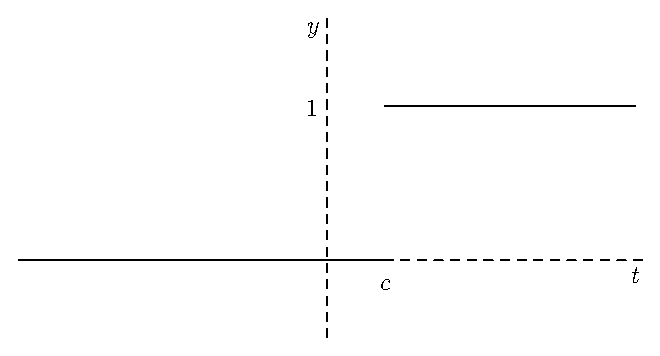
\includegraphics{201/step}
    \caption{Graph of the step function $u_c(t)$.}
    \label{step}
  \end{center}
\end{figure}

The Laplace transform of the step function is straightforward to calculate. If
we take $c>0$, then
\begin{align*}
\Laplace{}\(u_c(t)\) &=& \int_0^\infty u_c(t) e^{-st} dt
\\\nonumber
&=& \int_c^\infty e^{-st} dt
\\\nonumber
&=&\frac{e^{-cs}}{s}.
\end{align*}

The step function often shows up multiplied by other functions, as in the
following example.\\
\oexample{Solve the differential equation
\begin{align*}
y'=t u_c(t), \qquad y(0)=0
\end{align*}
using Laplace transforms.\\
}
{
Take the Laplace transform of both sides of the differential equation, yielding
\begin{align*}
sY &=& \Laplace{}\(t u_c(t)\) = \int_0^\infty t u_c(t) e^{-st} dt
= \int_c^\infty t e^{-st} dt
\\\nonumber
&=& \[t \frac{e^{-st}}{-s}\]_c^\infty - \int_c^\infty \frac{e^{-st}}{-s}dt
= \frac{-ce^{-sc}}{s} + \frac{e^{-sc}}{s^2}
\end{align*}
Thus,
\begin{align*}
Y = \frac{ce^{-sc}}{s} +\frac{e^{-sc}}{s^3}.
\end{align*}
From the table of  Laplace transforms, we know that
$\Laplace{}\(f(t-c)u_c(t)\)=e^{-cs}F(s)$, so
\begin{align*}
y = -c(t-c)u_c(t) + \frac{1}{2} (t-c)^2 u_c(t). \qed %FIXME: check
\end{align*}
}



\section{The Impulse Function}
While the step function describes functions which start suddenly (like turning
on a switch), the delta function, $\d(t)$, is slightly more complicated. It
describes processes that happen in an instant, like the impact from a hammer.
It is (loosely) defined as having the following properties:
\begin{align}
\boxed{
\delta(t) = \left\{ \begin{array}{ll}
         \infty & \mbox{if $t = 0$};\\
        0 & \mbox{if $t \neq 0$}.\end{array} \right.
}
\end{align}
and, for any function $f(t)$,
\begin{align}\label{deltaprop}
\boxed{\int_{-\infty}^\infty f(t) \delta(t)\, dt = f(0)}.
\end{align}
Approximations to the delta function are shown in figure~\ref{deltafig}.
\begin{figure}[htbp]
  \begin{center}
    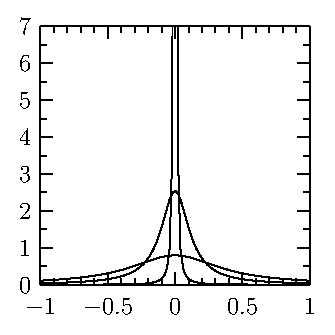
\includegraphics{201/delta}
    \caption{Approximations to $\d(x)$.}
    \label{deltafig}
  \end{center}
\end{figure}


\noindent\emph{Example}: Solve the following differential equation using
Laplace transforms.
\begin{align*}
2y'' + y' + 2y = \delta(t-5), \qquad y'(0)=y(0)=0
\end{align*}
\emph{Solution}: Taking the Laplace transform of both sides, we have
\begin{align}\label{exeq1}
\(2s^2 + s +2\) Y = e^{-5s}.
\end{align}
To see that the Laplace transform of $\delta(t-5)$ is $e^{-5s}$, consider the
definition of the Laplace transform:
\begin{align}
\mathcal{L}(\delta(t-5)) = \int_0^{\infty} e^{-st} \delta(t-5)\, dt.
\end{align}
If we let $\tau = t-5$, then this is the same as
\begin{align*}
\int_{-5}^{\infty} e^{-s(\tau+5)} \delta(\tau)\, d\tau .
\end{align*}
Then we apply equation (\ref{deltaprop}) to see that this is just $e^{-5s}$.

Going back to equation (\ref{exeq1}), solving for $Y$ and completing the
square yields
\begin{align*}
Y = \frac{e^{-5s}}{2} \( \frac{1}{\(s+\frac{1}{4}\)^2 + \frac{15}{16}} \).
\end{align*}
Finding the inverse transform is the hardest part of this process, but we can
break it up into smaller steps. We can just pull the $1/2$ out
because the Laplace transform is linear and then if we rearrange this, we get
%\begin{eqnarray}
\begin{align*}
Y = \frac{2}{\sqrt{15}}  \, e^{-5s}
\frac{\sqrt{\frac{15}{16}}}{\(s+\frac{1}{4}\)^2 + \frac{15}{16}}
= \frac{2}{\sqrt{15}}  \, e^{-5s} \,
\Laplace\[e^{\frac{-t}{4}}\sin\(\frac{\sqrt{15}}{4}t \) \]
%\end{eqnarray}
\end{align*}
Now we have an exponential term, $e^{-5s}$, times a term that is the Laplace
transform of $e^{\alpha t}\sin(\beta t)$ with $\alpha=1/4$ and
$\beta=\sqrt{{15}/{16}}$. So we will use the Laplace
transform table to see that $Y$ is the Laplace transform of
\begin{align*}
y=\frac{2}{\sqrt{15}}u_5(t) e^{\frac{-(t-5)}{4}}\sin\(\frac{\sqrt{15}}{4}(t-5)\).
\qed
\end{align*}

\section{Problems}
\begin{enumerate}
\item Solve the integro-differential equation
  \begin{align*}
  y(t) + \int_0^t y(v) (t-v) dv = 1.
  \end{align*}
  \hidesolution{
    \begin{align*}
    \int_0^t y(v) (t-v) dv = \int_0^t (t-v) y(v) dv = t \ast y(t)
    \end{align*}
    so this equation is
    \begin{align*}
    y(t) + t \ast y(t) = 1.
    \end{align*}
    Recall that
    \begin{align*}
    \Laplace \{f \ast g\} = \Laplace \{f\} \Laplace \{g\}
    \end{align*}
    so the Laplace transform of this equation is
    \begin{align*}
    \Laplace \{y(t)\} + \Laplace \{ t \ast y(t) \} &=& \Laplace \{1 \} \\
    \Laplace \{y(t)\} + \Laplace \{t\} \Laplace \{y(t)\} &=& \Laplace \{1\} \\
    Y(s) + \frac{1}{s^2} Y(s) &=& \frac{1}{s} \\
    \left( 1 + \frac{1}{s^2} \right) Y(s) &=& \frac{1}{s} \\
    \frac{s^2 + 1}{s^2} Y(s) &=& \frac{1}{s} \\
    Y(s) &=& \frac{s^2}{s(s^2+1)} \\
    Y(s) &=& \frac{s}{s^2+1}.
    \end{align*}
    Then taking the inverse transform yields
    \begin{align*}
    y(t) = \Laplace^{-1} \( \frac{s}{s^2+1} \) = \cos t.
    \end{align*}
  }

  \item
    Find the Laplace transform of
    \begin{align*}
    f =
    \left\{ \begin{array}{ll}
      e^t & \mbox{if $t < c$};\\
      t^2 & \mbox{if $t \geq c$}.
    \end{array} \right.
    \end{align*}
    \hidesolution{
      \begin{align*}
      \mathcal{L}(f)
      &=& \int_0^c e^t e^{-st} \, dt + \int_c^\infty t^2 e^{-st} \, dt
      \end{align*}
      The first integral is
      \begin{align*}
      \int_0^c e^t e^{-st} \, dt = \left.\frac{e^{(1-s)t}}{1-s}\right|_0^c
      =\frac{e^{(1-s)c}-1}{1-s}.
      \end{align*}
      The second integral requires two integrations-by-parts:
      \begin{align*}
      \int_c^\infty t^2 e^{-st} \, dt
      &=& \left. t^2 \frac{e^{-st}}{-s}\right|_c^\infty
      -2 \int_c^\infty t \frac{e^{-st}}{-s} \, dt
      \\
      &=&\frac{c^2}{s} +\frac{2}{s}
      \[
      t \left.\frac{e^{-st}}{-s}\right|_c^\infty
      - \int_c^\infty \frac{e^{-st}}{-s}\,dt
      \]
      \\
      &=&\frac{c^2}{s} + \frac{2c}{s^2} + \frac{2}{s^3}.
      \end{align*}
      The Laplace transform of $f$ is then the sum, i.e.,
      \begin{align*}
      \mathcal{L}(f) =
      \frac{e^{(1-s)c}-1}{1-s}
      + \frac{c^2}{s} + \frac{2c}{s^2} + \frac{2}{s^3}.
      \end{align*}
    }

\item
  Prove that $\Laplace(f*g)=F(s)G(s)$.
  \hidesolution{TODO: write solution.}

\item
  Solve $y'' = t u_c(t)$, $y(0)=y'(0)=0$, for $y(t)$ using Laplace transforms.
  \hidesolution{
    Note that $tu_c(t) = (t-c)u_c(t) +cu_c(t)$. Then,
    \begin{align*}
    s^2 Y = \frac{e^{-cs}}{s^2} + \frac{e^{-cs}}{s},
    \implies Y =  \frac{e^{-cs}}{s^4} + \frac{e^{-cs}}{s^3}
    \end{align*}
    so
    \begin{align*}
    y = u_c(t) \(\frac{t^3}{3!} + \frac{t^2}{2!}\).
    \end{align*}
  }

\item
  Solve the IVP
  \begin{align*}
  y'' + y = M\d(t-1), \qquad y'(0)=y(0)=0.
  \end{align*}
  \hidesolution{
  TODO: write solution.
  }

\end{enumerate}



\chapter{Solving Systems of Differential Equations}

Up to now, we could have solved every problem with the method of variation
of parameters. You've probably noticed that some questions are easier to
solve with certain techniques than with others, of course, but VoP will handle
any nonhomogeneous part, so long as you can calculate the integral. Here's
something that it won't handle:
\\

\noindent\emph{Example}:
Solve the system of initial value problems for both $x$ and $y$:
\begin{align*}
x' &=& -y \qquad x(0)=0 \\
y' &=& \phantom{-}x \qquad y(0)=1 \\
\end{align*}
Well, you can actually solve this by doing tricky things like taking the
derivative of one of the equations, but let's use Laplace transforms:
\\

\noindent\emph{Solution}: The Laplace transform of the original system is
\begin{align*}
sX &=& -Y \\
sY-1 &=&\phantom{-}X.
\end{align*}
Solving for $Y$ yields
\begin{align}
\label{syseg1}
sY -1 = \frac{-Y}{s} \quad \implies \quad Y = \frac{s}{s^2+1}.
\end{align}
Taking the inverse Laplace transform of equation (\ref{syseg1}) gives us
\begin{align*}
y(t) = \cos t.
\end{align*}
We can solve for $X$ in a similar way, or just notice that $x=y'$, i.e.\
\begin{align*}
x(t) = -\sin t
\end{align*}

Systems of differential equations model situations where there are two or
more quantities being evolved, such as heat and reaction rate, or predator and
prey populations. While they are obviously of great use, they can get
quite complicated as the number of variables increases (and are greatly
simplified by writing them in terms of matrices).\\


\noindent\emph{Example}: Solve the following system of differential equations:
\begin{align*}
x' - 3x + 2y = \sin t\\
4x -y' - y = \cos t
\end{align*}
with initial conditions $x(0)=y(0)=0$.
\\

\noindent\emph{Solution}:\\
We take the Laplace transform of each equation and put in the initial
conditions, which yields
\begin{align*}
sX - 3X +2Y = \frac{1}{s^2+1}\\
4X -sY -Y = \frac{s}{s^2+1}.
\end{align*}
We can solve the second equation for X:
\begin{align*}
X = \frac{1}{4}\(\frac{s}{s^2+1} + (s+1)Y\)
\end{align*}
Put this into the first equation, so
\begin{align*}
\(s-3\)\(\frac{1}{4} \frac{s}{s^2+1} + \frac{s+1}{4}Y\) +2Y
= \frac{1}{s^2+1}
\end{align*}
which gives
\begin{align}
\label{sysY}
Y &=& -\frac{(s-4)(s+1)}{(s^2+1)(s^2-2s+5)} \\ \nonumber
&=& \frac{11s +7}{10(s^2+1)} + \frac{-11s + 5}{10(s^2-2s+5)}  \\ \nonumber
&=& \frac{11s}{10(s^2+1)} + \frac{7}{10(s^2+1)} +
\frac{-11}{10}\frac{s-1}{(s-1)^2 + 2^2}
-  \frac{3}{10}\frac2{(s-1)^2 + 2^2}
\end{align}
by partial fractions and completing the square in the last two terms. We are
now in a position to use an inverse Laplace transform to get $y(t)$:
\begin{align*}
y(t) = \frac{7}{10} \sin t + \frac{11}{10} \cos t
- \frac{11}{10}e^{t}\cos 2t - \frac{3}{10}e^{t}\sin 2t
\end{align*}
It now remains to solve for $x(t)$. We use the solution for $X$
and the Laplace transform of $y$. This is to say
\begin{align}
\label{sysX}
X &=& \frac{1}{4}\(\frac{s}{s^2+1} + (s+1)Y\)\\ \nonumber
 &=& \frac{-1 + 7s}{10(s^2+1)} + \frac{-7s + 15}{10(s^2-2s+5)} \\ \nonumber
 &=& \frac{7s}{10(s^2+1)} + \frac{-1}{10(s^2+1)} + \frac{-7}{10}
\frac{s-1} {(s-1)^2 + 2^2} +  \frac{2}{5}\frac{2}{(s-1)^2 + 2^2}
\end{align}
So we can now use an inverse Laplace transform to get $x(t)$.
\begin{align*}
x(t) = \frac{-1}{10} \sin t + \frac{7}{10} \cos t - \frac{7}{10}e^{t}\cos 2t
+ \frac{2}{5}e^{t}\sin 2t
\end{align*}

Alternatively, we could have solved this as a linear system, since
\begin{align*}
\[ \begin{array}{ll}
    (s-3) & 2\\
    4 & -(s+1)
  \end{array} \]
\( \begin{array}{l}
    X\\
    Y
  \end{array} \)
=
\( \begin{array}{l}
    \frac{1}{s^2+1}\\
    \frac{s}{s^2+1}
  \end{array} \)
\end{align*}
which is easily solved for $X$ and $Y$ to give
\begin{align*}
\( \begin{array}{l}
    X\\
    Y
  \end{array} \)
=
\frac{1}{s^2+1} \cdot \frac{1}{s^2-2s+5}
\( \begin{array}{l}
    3s+1\\
    s^2 -3s -4
  \end{array} \),
\end{align*}
which brings us to equations (\ref{sysY}) and (\ref{sysX}) with a lot less
work. \qed

\section{Problems}

\begin{enumerate}
  \item Solve the following system of differential equations:
    \begin{align*}
    \begin{array}{ll}
      x'=z, & \qquad x(0)=0\\
      y'=x, &\qquad y(0)=0 \\
      z'=y, &\qquad z(0)=1.
    \end{array}
    \end{align*}
    \hidesolution{
      Note: For the quiz, computing just $z(t)$ should be sufficient, since this
      takes students about 40 minutes.\\

      The Laplace transform gives us
      \begin{align*}
      sX &=& Z \\
      sY &=& X \\
      sZ-1 &=& Y
      \end{align*}
      Solving for $Z$, we have
      \begin{align*}
      Z &=& \frac{s^2}{s^3-1}
      = \frac{1}{3}\frac{1}{s-1}
      + \frac{1}{3} \frac{2s+1}{s^2 + s+ 1}\\
      &=& \frac{1}{3}\frac{1}{s-1}
      + \frac{1}{3} \frac{2s+1}{(s+\half)^2+ \frac{3}{4}}
      = \frac{1}{3}\frac{1}{s-1}
      + \frac{2}{3} \frac{s+\half}{(s+\half)^2+ \frac{3}{4}}
      \end{align*}
      which has inverse Laplace transformation
      \begin{align*}
      z = \frac{1}{3}e^t
      + \frac{2}{3}e^{-\frac{t}{2}} \cos \frac{\sqrt{3}}{2} t.
      \end{align*}
      Similarly, $sX=Z$ implies that
      \begin{align*}
      X = \frac{s}{s^3 -1}
      = \frac{1}{3}\frac{1}{s-1} - \frac{1}{3}\frac{s-1}{s^2+s+1}
      = \frac{1}{3}\frac{1}{s-1}
      - \frac{1}{3}\frac{s+\half}{(s+\half)^2+\frac{3}{4}}
      - \frac{1}{3}\frac{-3}{2}\frac{2}{\sqrt{3}}
      \frac{\sqrt{3}/2}{(s+\half)^2+\frac{3}{4}}
      \end{align*}
      so
      \begin{align*}
      x = \frac{e^t}{3}
      -e^{\frac{-t}{2}}\(
      \frac{1}{3}\cos \frac{\sqrt{3}}{2}t
      +\frac{1}{\sqrt{3}}\sin \frac{\sqrt{3}}{2}t
      \),
      \end{align*}
      and $sY=X$ implies that
      \begin{align*}
      Y = \frac{1}{s^3-1}
      = \frac{1}{3}\frac{1}{s-1} - \frac{1}{3}\frac{s+2}{s^2+s+1}
      = \frac{1}{3}\frac{1}{s-1}
      - \frac{1}{3}\frac{s+\half}{(s+\half)^2+\frac{3}{4}}
      - \frac{1}{3}\frac{3}{2}\frac{2}{\sqrt{3}}
      \frac{\sqrt{3}/2}{(s+\half)^2+\frac{3}{4}}
      \end{align*}
      so
      \begin{align*}
      Y = \frac{e^t}{3}
      +e^{\frac{-t}{2}}\(
      \frac{1}{3}\cos \frac{\sqrt{3}}{2}t
      -\frac{1}{\sqrt{3}}\sin \frac{\sqrt{3}}{2}t
      \).\qed
      \end{align*}
    }

  \item
    Solve the following system of differential equations
    \begin{align*}
    x' -y = e^t, \qquad x(0)=1.
    \\
    y' + x = e^t, \qquad y(0)=0.
    \end{align*}
    \hidesolution{
      The transform gives us
      \begin{align*}
      sX -1 -Y = \frac{1}{s-1}
      \\
      sY + X = \frac{1}{s-1}
      \end{align*}
      so
      \begin{align*}
      s^2 Y  + Y = \frac{-1}{s-1} -1 + \frac{s}{s-1}
      =- \frac{1}{s-1} -1 + \frac{s-1}{s-1} - \frac{1}{s-1}
      = \frac{-2}{s-1}.
      \end{align*}
      Thus,
      \begin{align*}
      Y = \frac{-2}{3} \(-\frac{s+1}{s^2+1} + \frac{1}{s-1} \)
      \end{align*}
      so
      \begin{align*}
      y = \frac{2}{3}\sin t + \frac{2}{3}\cos t - \frac{2}{3}e^t
      \text{ and } x = e^t-y'
      = -\frac{2}{3}\cos t + \frac{2}{3} \sin t + \frac{5}{3}e^t
      .\qed
      \end{align*}

    }

    \item
      Solve the system of differential equations
      \begin{align*}
      x'+y=0,\qquad x(0)=1
      \\
      y' = 2 \cosh(2t),\qquad y(0)=1
      \end{align*}
      \hidesolution{
      The second DE has transform
      \begin{align*}
      sY -1 = 6 \frac{s}{s^2-4} \implies Y =  6 \frac{1}{s^2-4} + \frac{1}{s}
      \end{align*}
      so
      \begin{align*}
      y = \sinh(t) +1
      \end{align*}
      and
      \begin{align*}
      x = \int \sinh(t) +1 dt = \cosh t +t +C
      \end{align*}
      with $C=0$ matching the initial condition. \qed
      }

\end{enumerate}


\chapter{Series Solutions to DEs}

A smooth function $f(t)$ can be approximated near a point $t=a$ by looking
at its derivatives. In fact, if $f$ is smooth enough, its value at any
given $t$ can be entirely determined by its behaviour at $t=a$.

The most basic approximation that we can make is that the function stays
constant. For example, a good guess for the temperature in ten minutes would
be what the temperature is now. That is, we approximate $f$ as
\begin{align*}
f(t) \approx f_0(t) = f(a).
\end{align*}
Now, it may be that the sun is shining, so we expect it to heat up. Then our
next approximation is to account for this using $f'(a)$, i.e.\
\begin{align*}
f(t) \approx f_1(t) = f(a) + f'(a) (t-a).
\end{align*}
As the sun sets, the rate of heating changes, so we need to add a term with
$f''(a)$, which gives us
\begin{align*}
f(t) \approx f_2(t) = f(a) + f'(a) (t-a) + \frac{f''(a)}{2}\(t-a\)^2,
\end{align*}
and so on. This is called a \emph{Taylor Polynomial Approximation} (or simply a
Taylor polynomial). It's easy to deal with both analytically and numerically,
and it can be used to get at least a basic understanding of just about any IVP.

The $n$th degree Taylor polynomial is
\begin{align}
\boxed{f_n(t) = f(a) + f'(a)(t-a) + \dots + \frac{f^{(n)}(a)}{n!} (t-a)^n
= \sum_{i=0}^n \frac{f^{(i)}(a)}{i!}(t-a)^i},
\end{align}
and it exists for any function $f$ whose first $n$ derivatives are smooth for
$t\in [a,t]$.
Let $R_n(t) = f(t) -f_n(t)$ denote the error associated with the $n$th Taylor
polynomial. Then, Taylor's theorem states that there exists a number
$\xi \in [a,t]$ where
\begin{align}
\boxed{R_n(t) = \frac{f^{(n+1)}(\xi)}{(n+1)!}(t-a)^{n+1}}.
\end{align}
So long as $\lim_{n\rightarrow \infty} R_n(t) =0$, $f_n$ will be a better and
better approximation as $n$ increases.


The Taylor series of $f$ is the limit of $f_n$ as $n\rightarrow\infty$, which is
\begin{align}
\boxed{\sum_{i=0}^\infty \frac{f^{(i)}(a)}{i!}(t-a)^i}.
\end{align}
The Taylor series for $f$ exists as long as every derivative of $f$ is
continuous (i.e.\ $f$ is \emph{analytic}), and is equal to $f$ if their
difference is zero (i.e.\ $\lim_{n\rightarrow \infty} R_n(t) =0$). Since these
things are equal, we can use this to solve equations. Of course, we need to
make sure that these series converge in order for our solution to make sense.
What's more, if $f$ is analytic, then the derivative of the sum is the sum
of the derivatives, which can greatly simplify things.\\

\oexample{
  Find the Taylor series for $f=e^x$ about $x=0$ and its interval of
  convergence.
}{
  First, we need to find the derivatives of $e^x$. This is easy, since
  \begin{align*}
  f^{(n)}(x) = \frac{d^n}{dx^n}e^x = e^x.
  \end{align*}
  Thus, $f^{(n)}(0)=e^0=1$, so the Taylor series is given by
  \begin{align*}
  \sum_{n=0}^\infty \frac{1}{n!} x^n.
  \end{align*}
  For what values of $x$ will this series converge? To determine this, we'll
  have to use a convergence test. Letting $A=\sum_{n=0}^\infty a_n$
  $B=\sum_{n=0}^\infty b_n$ be two series, our test are:
  \begin{enumerate}
  \item The comparison test: if
    $\lim_{n \rightarrow \infty} \abs{a_n/b_n} \in (0,\infty)$, then $A$
    converges if and only if $B$ converges.
  \item The ratio test: if
    $\lim_{n\rightarrow\infty}\abs{\frac{a_{n+1}}{a_n}}=c < 1$, then $A$
    converges.
  \item The root test: if $\lim_{n\rightarrow\infty}\abs{a_n}^{1/n}=c < 1$,
    then $A$ converges.
  \item The integral test: if there is a function $f$ with $f(n)=a_n$, then
    $A$ converges if and only if $\int_0^\infty f(t) dt$ is finite.
  \item The alternating series test: if $a_n = (-1)^n c_n$, then $A$
    converges so long as $\lim_{n\rightarrow\infty}c_n=0$ and each $c_n$ is
    smaller than $c_{n-1}$.
  \end{enumerate}
  Let's try the ratio test. That is, fix $x$ and look at
  \begin{align*}
  \lim_{n\rightarrow\infty} \frac{a_{n+1}}{a_n}
  = \lim_{n\rightarrow\infty}\frac{x^{n+1}/(n+1)!}{x^n/n!}
  =\lim_{n\rightarrow\infty}\frac{x}{n+1} =0 < 1.
  \end{align*}
  That is, for any $x\in \mathbb{R}$, $n+1$ will eventually be greater than
  $x$.  Thus, the limit is zero, and the series converges for all
  $x \in (-\infty,\infty) =\mathbb{R}$. \qed
}

In the above example, the series converged everywhere. This isn't always
the case: often, a series solution to a differential equation is only
valid in some neighbourhood of the initial conditions, and the series
becomes divergent when $\abs{t-a} > r$, and we call $r$ the radius of
convergence.\\

\oexample{
  Find the radius of convergence for the Taylor series for $f=\arctan(x)$
  about $x=0$.\\
}
{
  The Taylor series for $\arctan(z)$ is
  \begin{align*}
  \sum_{n=0}^\infty \frac{(-1)^n z^{2n+1}}{2n+1}
  \end{align*}
  Using the ratio test again, we look at
  \begin{align*}
  \abs{\frac{a_{n+1}}{a_n}} = \frac{z^{2(n+1)+1}/(2(n+1)+1)}{z^{2n+1}/(2n+1)}
  = \frac{z^2}{(2n+3)/(2n+1)}\rightarrow z^2
  \end{align*}
  Clearly, this limit is only less than one if $\abs{z}<1$. We still need to
  check the case when $\abs{z}=1$. This is pretty easy to do, since if $z=1$,
  the series is just
  \begin{align*}
  \sum_{n=0}^\infty \frac{(-1)^n}{2n+1},
  \end{align*}
  which converges by the alternating series test. Similarly, the series
  converges if $z=-1$. Thus, the interval of convergence is $\[-1,1\]$.
  \qed
}

Now that we can calculate Taylor series and know when they are valid, we
can use them to calculate solutions to differential equations. To simplify
matters, we will restrict ourselves to initial value problems
which begin at $t=0$, so that $a=0$ in all the above formulae. Now, we can
express the solution $y(t)$ as a Taylor series,
\begin{align*}
y = \sum_{n=0}^\infty a_n t^n .
\end{align*}
We assume that this solution is analytic, so we can take the derivative of the
series term-by-term. That is,
\begin{align*}
\dd{y}{t} = \dd{}{t}\sum_{n=0}^\infty a_n t^n
= \sum_{n=0}^\infty \dd{(a_n t^n)}{t} = \sum_{n=0}^\infty a_n n t^{n-1}
= \sum_{n=1}^\infty a_n n t^{n-1}
\end{align*}
(the last equality is because when $n=0$ we have that $a_n n t^{n-1}=0$, so we
can ignore the term with $n=0$). Since we know that $a_0=y(0)$, and $y(0)$ is
given by the initial conditions, we can solve for the rest of the $a_n$
recursively.\\
\oexample{Determine the solution to the IVP
\begin{align*}
y'(t) = t^2 +t, \qquad y(0)=1
\end{align*}
using a Taylor series for $y$.\\
}
{
  Let
  \begin{align*}
  y =\sum_{n=0}^\infty a_n t^n.
  \end{align*}
  Then, $a_0=y(0)=1$, and
  \begin{align*}
  y'(t) = \sum_{n=1}^\infty a_n n  t^{n-1} = t^2 +t.
  \end{align*}
  Matching like powers of $t$, we have
  \begin{align*}
  2 a_2 t = t, \qquad 3 a_3 t^2 = t^2
  \end{align*}
  and $a_n n t^n =0$ for $n=1$ and all $n \geq 4$. Thus, $a_1 =0$, $a_2=\half$,
  and $a_3 = \frac{1}{3}$. The solution is then
  \begin{align*}
  y(t) = 1 +\frac{t^2}{2} +\frac{t^3}{3}.
  \end{align*}
}
It was easy to isolate all of the $a_n$'s in the previous example, since $y'$
appeared alone in the IVP. It's usually necessary to solve for $a_n$
recursively.\\
\oexample{
  Solve the IVP
  \begin{align*}
  y'' = -y, \qquad y(0) =1, \qquad y'(0)=0.
  \end{align*}
  using a Taylor series for $y$.\\
}
{
  Again, let $y=\sum_{n=0}^\infty a_n t^n$. Then
  \begin{align*}
  y'' = \sum_{n=2}^\infty a_n n (n-1)t^{n-2}.
  \end{align*}
  The differential equation is then
  \begin{align}
  \label{serieseg}
  \sum_{n=2}^\infty a_n n (n-1)t^{n-2} = -\sum_{n=0}^\infty a_n t^n
  \end{align}
  If we set $m=n-2$, then we can shift the summation index on the LHS to start
  at zero. That is,
  \begin{align*}
  y'' = \sum_{n=2}^\infty a_n n (n-1)t^{n-2}
  = \sum_{m=0}^\infty a_{m+2}(m+2)(m+1)t^m.
  \end{align*}
  This makes it much easier to solve \eqref{serieseg}, since we now have
  \begin{align*}
  \sum_{m=0}^\infty a_{m+2}(m+2)(m+1)t^m =  -\sum_{n=0}^\infty a_n t^n
%  \end{align*}
%  \begin{align*}
  \implies \sum_{n=0}^\infty \[a_{n+2}(n+2)(n+1) +a_n \]t^n =0
  \end{align*}
  In order for this to hold for all $t$ in a neighbourhood of $t=0$, it must
  be that
  \begin{align}
  \label{seriesrec}
  a_{n+2}(n+2)(n+1) +a_n =0.
  \end{align}
  From the initial conditions, we have $a_0=1$ and $a_1=0$. We can solve
  for $a_2$ by setting $n=0$ in equation \eqref{seriesrec}, which yields
  \begin{align*}
  a_2 \times 2 \times 1 = -1, \implies a_2=-\half.
  \end{align*}
  If we have $n$ even, then $n=2p$, and
  \begin{align*}
  a_{2p} = -\frac{a_{2p-2}}{2p(2p-1)} = \frac{a_{2p-4}}{2p(2p-1)(2p-3)(2p-4)}
  = \dots
  = \frac{(-1)^p a_0}{(2p)!} =\frac{(-1)^p}{(2p)!}
  \end{align*}
  It's easy to see that $a_3=0$, and, in fact, $a_n=0$ if $n$ is odd. Since
  we now know the values for all the $a_n$, we can write the solution:
  \begin{align*}
  y(t) = \sum_{n=0}^\infty t^n
  \left\{\begin{array}{ll}
    \frac{(-1)^{n/2}}{n!} & \mbox{if $n$ is even};\\
    0 & \mbox{if $n$ is odd}.
  \end{array} \right.
  = \sum_{p=0}^\infty \frac{(-1)^p t^{2p}}{(2p)!}. \qed
 \end{align*}
 You may recall from previous classes that this is just the Taylor series
 for $\cos t$.
}




\section{Problems}
\begin{enumerate}
\item Determine the convergence set of the series
  \begin{align*}
  \sum_{n=0}^\infty \frac{3^n}{n} (x-2)^n.
  \end{align*}
  \hidesolution{
    For this series $a_n = \frac{3^n}{n}$ and $x_0 = 2$, so
    \begin{align*}
    L = \lim_{n \to \infty} \left| \frac{a_{n+1}}{a_n} \right|
    = \lim_{n \to \infty} \left| \frac{3^{n+1}}{n+1} / \frac{3^n}{n} \right|
    = \lim_{n \to \infty}
    \left| \frac{3 \cdot 3^n}{n+1} \times \frac{n}{3^n} \right|
    = \lim_{n \to \infty} \left| 3 \frac{n}{n+1} \right|
    = 3 \lim_{n \to \infty} \frac{n}{n+1}
    = 3
    \end{align*}
    and then
    \begin{align*}
    \rho = \frac{1}{L} = \frac{1}{3}.
    \end{align*}
    So the series converges (absolutely) on
    \begin{align*}
    (x_0 - \rho, x_0 + \rho) = \left( 2 - \frac{1}{3}, 2 + \frac{1}{3} \right)
    = \left( \frac{5}{3}, \frac{7}{3} \right).
    \end{align*}
    It remains to check if the series converges at the endpoints of this
    interval.  At $x = \frac{5}{3}$, we have
    \begin{align*}
    \sum_{n=0}^\infty \frac{3^n}{n} \left( \frac{5}{3} - 2 \right)^n
    = \sum_{n=0}^\infty \frac{3^n}{n} \left( \frac{-1}{3} \right)^n
    = \sum_{n=0}^\infty \frac{3^n}{n} \times \frac{(-1)^n}{3^n}
    = \sum_{n=0}^\infty \frac{(-1)^n}{n}
    \end{align*}
    which is the alternating harmonic series which converges (recall that an
    alternating series converges $\iff$ the terms go to 0),
    and at $x = \frac{7}{3}$ we have
    \begin{align*}
    \sum_{n=0}^\infty \frac{3^n}{n} \left( \frac{7}{3} - 2 \right)^n
    = \sum_{n=0}^\infty \frac{3^n}{n} \left( \frac{1}{3} \right)^n
    = \sum_{n=0}^\infty \frac{1}{n}
    \end{align*}
    which is the harmonic series which diverges. So the convergence set is
    \begin{align*}
    \left[ \frac{5}{3}, \frac{7}{3} \right).
    \end{align*}
  }

  \item
    Determine the first four non-zero terms of the Taylor series of the
    solution to the Chebyshev equation,
    \begin{align*}
    (1-x^2)y'' - xy' +p^2 y=0
    \end{align*}
    with initial conditions $y(0)=a_0$, $y'(0)=a_1$.
    \hidesolution{
      TODO: write the solution
    }

  \item
    Determine the fourth degree Taylor polynomial for the solution to
    \begin{align*}
    (y')^2 + y = e^x, \qquad y(0)=0.
    \end{align*}
    \hidesolution{
      The first four terms of $y'$ are $a_1 + 2 a_2 x +3 a_3 x^2 + 4 a_4 x^3$.
      The first four terms of $y'^2$ are therefore
      \begin{align*}
      (y') + y \approx a_0+a_1^2 + x\(a_1 +4 a_1 a_2 \)
      + x^2 \(a_2+ 4a_2^2+6 a_1 a_3 \)
      +x^3\(a_3 + 8a_1 a_4 +12 a_2 a_3 \)
      \end{align*}
      and equal
      \begin{align*}
      e^x \approx 1 + x + \frac{x^2}{2} + \frac{x^3}{6}
      \end{align*}
      Matching order-by-order, we have
      \begin{align*}
      \begin{array}{ll}
	\O(1): & a_0 + a_1^2 =1 \\
	\O(x): & a_1(1+ 4 a_2) =1\\
	\O(x^2): & a_2 + 4a_2^2 + 6 a_1 a_3 =\half \\
	\O(x^3): & a_3 + 8 a_1 a_4 + 12 a_2 a_3=\frac{1}{6} \\
      \end{array}
      \end{align*}
      Subbing back into these equations, we get
      \begin{align*}
      a_1=1, \qquad a_2 =0, \qquad a_3=\frac{1}{12}, \qquad a_4=\frac{1}{96},
      \end{align*}
      and
      \begin{equation*}
        y(x) \approx x + \frac{x^3}{12} + \frac{x^4}{96}.
      \end{equation*}
    }

  \item
    Solve
    \begin{align*}
    y' = \frac{1}{1+x^2}, \qquad y(0)=0
    \end{align*}
    using a Taylor series. Do not leave your solution as an infinite series,
    but equate it to a known function.
    \hidesolution{
      This is just $y(x)=\arctan x$.
    }

%too complicated--needs help
% \item
%    The pendulum is often approximated as a harmonic oscillator. The full
%    system is nonlinear in $y$, since
%    \be
%    y''=-\sin y,
%    \end{align}
%    which reduces to the usual case, $y''=-y$, for small $y$. A slightly
%    better approximation would be to approximate $\sin$ to higher order, as in
%    \be
%    \label{pend3}
%    y''=-y + \frac{y^3}{3!}.
%    \end{align}
%    Provide a third-order Taylor polynomial approximation to the solution of
%    \eqref{pend3}.
%
%    If we take \eqref{pend3} and multiply it by $y'$, we can get the energy
%    equation for the system, namely
%    \be
%    y' y'' = \ddt{y'^2/2}
%    = \ddt{}\int^{y(t)}\(-\hat{y} + \frac{\hat{y}^3}{3!}\) d\hat{y}.
%    \end{align}
%    Thus, the energy of the system, $E=\frac{y'^2}{2}
%    + \int^{y(t)}\(\hat{y} - \frac{\hat{y}^3}{3!}\) d\hat{y}$, is conserved,
%    since
%    \be
%    \ddt{}\(\frac{y'^2}{2}
%    + \int^{y(t)}\(\hat{y} - \frac{\hat{y}^3}{3!}\) d\hat{y}\) =0.
%    \end{align}
%    Based on the conservation of energy, what do you expect to happen at large
%    $y$? Why might $y''=-y$ be a better approximation at large $y$ than
%    $y''=-y + {y^3}/{3!}$ is?
%    \hidesolution{
%      TODO: work out the approximation
%
%      The reason that the third-order approximation breaks down is that
%      the energy goes to $-\infty$ for large $\abs{y}$, so the solution will
%      grow unboundedly.
%    }

  \item
    Give a recursion formula for $a_n$ if
    \begin{align*}
    a_{3n+1} = \frac{a_1}{(3n+1)\times (3n) \times (3n-2) \dots
      6 \times 4 \times \times 3}.
    \end{align*}

  \item
    Given the recursion relationship
    \begin{align*}
    a_n = \frac{-2}{n^2}a_{n-1},
    \end{align*}
    find $a_n$ explicitly.

  \item
    Given the recursion relationship
    \begin{align*}
    a_{n+4} = \frac{-k^2}{(n+4)(n+3)} a_{n-1},
    \end{align*}
    with $k$ a constant, find $a_n$ explicitly.

  \item Solve the differential equation
    \begin{align*}
    y'' - 2 x y' + \l y=0,
    \end{align*}
    with $\l$ a constant, using a Taylor series about $x=0$. For what values
    of $\l$ is the solution a polynomial?

\end{enumerate}



\chapter{Series Solutions to DEs at Regular Singular Points}
%Let $p(t), q(t)$ be analytic functions (ie, they admit power series
%representations).
Differential equations of the form
\begin{align}
\label{singode}
y'' + p(t)y' + q(t)y=0
\end{align}
can behave poorly at $t=0$, and may not admit solutions of the form
$y(t) =\sum_{n=0}^\infty a_n t^n$. However, we can still solve these problem
by modifying the series expansion. The easiest case is when the singular
point is a regular singular point, for which we use \emph{the method of
Froebenius}.

The point $t=0$ is a \emph{singular point} if either
$\lim_{t \rightarrow 0}p(t)=\infty$ or  $lim_{t \rightarrow 0}q(t)=\infty$.

The point $t=0$ is a \emph{regular singular point} of \eqref{singode} if
the two limits $\lim_{t\rightarrow 0} t p(t) =p_0$
and $\lim_{t\rightarrow 0} t^2 q(t) =q_0$
exist and are finite. Series solutions at regular singular points are of the
form
\begin{align}
\boxed{y(t) = \sum_{n=0}^\infty a_n t^{n+r}},
\end{align}
for some $r\in\mathbb{C}$ such that $a_0 \neq 0$.

Since we now have one more variable for which to solve (i.e.\ $r$ in addition
to $a_0, a_1,\dots$), we require one more equation in order to determine the
solution uniquely. Then if we take the first and second derivative of
$y(t) = \sum_{n=0}^\infty a_n t^{n+r}$ and put them into the left-hand side of
equation \eqref{singode}, we can see that the
leading-order (which is to say the $t^{r-2}$) coefficient is
\begin{align*}
a_0 r(r-1)t^{r-2} + a_0 \frac{p_0}{t} r t^{r-1} + a_0 \frac{q_0}{t^2} t^r
\end{align*}
In order to satisfy equation \eqref{singode}, this equation must equal $0$.
We can multiply by $t^2$ and since $a_0 \neq 0$, we see that
\begin{align}
\boxed{\implies r(r-1) + p_0 r  + q_0=0}.
\end{align}
This is called the \emph{indicial equation}. It's a quadratic so it has two
solutions, $r=r_1,r_2$.

If we have two distinct roots with $Re(r_1) > Re(r_2)$, we're fine, and we
have two linearly independent solutions
\begin{align}
\boxed{y_1(t) = \sum_{n=0}^\infty a_n t^{n+r_1}}
\quad\mbox{  and  }\quad
\boxed{y_2(t) = \sum_{n=0}^\infty b_n t^{n+r_2}}.
\end{align}
If $r_1=r_2$, then our solutions are
\begin{align}
\boxed{y_1(t) = \sum_{n=0}^\infty a_n t^{n+r_1}}
\quad\mbox{  and  }\quad
\boxed{y_2(t) = \ln(t) y_1(t) + \sum_{n=0}^\infty b_n t^{n+r_1}}.
\end{align}
If $r_1-r_2$ is an integer, then we have yet another possibility, i.e.\ that
\begin{align}
\boxed{y_1(t) = \sum_{n=0}^\infty a_n t^{n+r_1}}
\quad\mbox{  and  }\quad
\boxed{y_2(t) = C\ln(t) y_1(t) + \sum_{n=0}^\infty b_n t^{n+r_1}},
\end{align}
for some constant $C\in\mathbb{R}$.

Once one has determined $r_1$ and $r_2$, the constants $a_n$ and $b_n$ can
be determined by matching powers as per the previous section.

% \oexample{
%   Consider Bessel's equation,
%   \begin{align}
%   \label{bessel}
%   t^2 y'' + ty' + (t^2-\alpha^2)y=0.
%   \end{align}
% }{
%   We can divide Bessel's equation by $t^2$ to get it in the form of
%   \eqref{singode}, that is
%   \begin{align*}
%   y''  + \frac{1}{t}y' + \(1-\frac{\alpha^2}{t^2}\)y=0,
%   \end{align*}
%   which is clearly singular. We can identify $p=1/t$, and
%   $q=1-\frac{\alpha^2}{t^2}$. Then,
%   \begin{align*}
%   p_0 = \lim_{t\rightarrow 0} t p(t) =1, \quad \text{and}\quad
%   q_0 = \lim_{t\rightarrow 0} t^2 q(t) =-\alpha^2.
%   \end{align*}
%   The indicial equation is then
%   $r(r-1) +r -\alpha^2 =0 \implies r_{1,2} = \pm \alpha$.  Thus,
%   \begin{align*}
%   y_1\phantom{''} &=& \sum_{n=0}^\infty a_n t^{n+\alpha} \\
%   y_1'\phantom{'}  &=& \sum_{n=0}^\infty a_n (n+\alpha)t^{n+\alpha-1}, \\
%   y_1'' &=& \sum_{n=0}^\infty a_n (n+\alpha)(n+\alpha-1)t^{n+\alpha-2}.
%   \end{align*}
%   Putting this into \eqref{bessel}, we have
%   \begin{align*}
%   \sum_{n=0}^\infty a_n\[(n+\a)(n+\a-1) + (n+\a) - \a^2  \]t^{n+\alpha}
%   + \sum_{n=0}^\infty a_n t^{n+2+\alpha}=0.
%   \end{align*}
%   Changing the index of the second sum, we have
%   \begin{align*}
%   \sum_{n=0}^\infty a_n\[(n+\a)(n+\a-1) + (n+\a) - \a^2  \]t^{n+\alpha}
%   + \sum_{n=2}^\infty a_{n-2} t^{n+\alpha}=0.
%   \end{align*}
%   The $a_0$ and $a_1$ terms are determined by initial conditions. For
%   $n\geq 2$, the terms must cancel, so we have
%   \begin{align*}
%   a_n\[\(n+\a\)^2 - \a^2\]t^{n+\alpha}  + a_{n-2} t^{n+\alpha}=0
%   \end{align*}
%   which implies that
%   \begin{align*}
%   a_n = \frac{-a_{n-2}}{\(n+\a\)^2 - \a^2} =  \frac{-a_{n-2}}{n(n+ 2\a)}.
%   \end{align*}
%   Associating $y_1$ with $a_0=1$ and $a_1=0$, we can set $n=2m$, so the
%   recursion relationship is
%   \begin{align}
%   a_{2m} = \frac{-a_{2(m-1)}}{2m (2m+2\a)} = \frac{-a_{2(m-1)}}{2^2m (m+\a)}.
%   \end{align}
%   Solving the recursion relationship then yields
%   \begin{align}
%   a_{2m} = \frac{(-1)^ma_0}{2^{2m}m! (m+\a)(m+\a-1)\dots(1+\a)}.
%   \end{align}
%   The solution is then
%   \begin{align}
%   \label{bessel1}
%   y_1 = \sum_{m=0}^\infty
%   \frac{(-1)^m}{2^{2m}m! (m+\a)(m+\a-1)\dots(1+\a)(\a)} t^{m+\alpha}.  \qed
%   \end{align}
% We can simplify this a little by setting $a_0=1/(2^\a\G(\a+1))$. Then we would
% get the standard form of Bessel's function of the first kind of order $\a$,
%   \begin{align*}
%   J_\alpha(t) = \sum_{n=0}^\infty \frac{(-1)^n}{n!\G(1-\a+n)}
%   \(\frac{t}{2}\)^{2n-\a}.
%   \end{align*}
% Here $\G(x)$ is called the Gamma function and it is just an extension of the
% factorial function. So in particular, when $\alpha=0$, we get
%   \begin{align*}
%   J_0(t) = \sum_{n=0}^\infty \frac{(-1)^n t^{2n}}{2^{2n}(n!)^2}.
%   \end{align*}
% % Too messy and complicated- fixed above
% %  Now, we can simplify this slightly, by using the gamma function. The
% %  Gamma function,
% %  \be
% %  \G(x) = \int_0^\infty t^{x-1} e^{-t} \, dt,
% %  \end{align}
% %  is a generalization of the factorial. The key step is that
% %  \be
% %  \G(x+1) = x \G(x),
% %  \end{align}
% %  which can be derived using integration by parts. If $x$ is an integer, this
% %  gives us $\G(x+1)=x!$, since $\G(0)=1$. If we set $x=m+\a+1$, then
% %  \be
% %  \G(m+\a+1) &=& (m+\a) \G(m+\a) = (m+\a)(m+\a-1)\G(m+\a-1) = \dots \\\nonumber
% %  &=& (m+\a)(m+\a-1) \dots (2+\a)(1+\a)\G(\a+1).
% %  \end{align}
% %  We can then write \eqref{bessel1} as
% %  \be
% %  y_1 = \sum_{m=0}^\infty
% %  \frac{(-1)^m}{2^{2m}m! \G(m+\a+1)/\G(\a+1)} t^{m+\alpha}.
% %  \end{align}
% %
% %  Setting $a_0=1/(2^\a\G(\a+1))$, we have the standard form of Bessel's
% %  function
% %  of the first kind of order $\a$,
% %  \be
% %  J_\alpha(t) = \sum_{n=0}^\infty \frac{(-1)^n}{n!\G(1-\a+n)}
% %  \(\frac{t}{2}\)^{2n-\a}. \qed
% %  \end{align}
% }



\section{Problems}

\begin{enumerate}

  \item Find a general solution to the Cauchy-Euler (equidimensional) equation,
    \begin{align*}
    (\pi x)^2 y'' (x) + \pi(\pi-2)xy' (x) + y(x) = 0, \quad x > 0.
    \end{align*}
    \hidesolution{
      Rewrite this equation as
      \begin{align*}
      \pi^2 x^2 y'' (x) + (\pi^2 - 2\pi)xy' (x) + y(x) = 0.
      \end{align*}
      We substitute $y = x^r$ to find a solution. The indicial equation is
      \begin{align*}
      \pi^2 r^2 + (\pi^2 - 2\pi - \pi^2) r + 1 = \pi^2 r^2 - 2 \pi r + 1
      = (\pi r - 1)^2 = 0
      \end{align*}
      which has repeated root $r = \frac{1}{\pi}$.  So a general solution is
      \begin{align*}
      y(x) = C_1 x^\frac{1}{\pi} + C_2 x^\frac{1}{\pi} \ln x
      = C_1 \sqrt[\pi]{x} + C_2 \sqrt[\pi]{x} \ln x, \quad x > 0.
      \end{align*}
    }

  \item Find the solution to Bessel's equation corresponding to $r=-\a$,
    assuming that $2\a$ is not an integer.
    \hidesolution{
      TODO: add solution
    }

  \item Find the first solution (i.e.\ $y_1$ in the above notation) to the
    differential equation
    \begin{align*}
    x^2 y'' - xy' + (1-x)y=0
    \end{align*}
    \hidesolution{
      We have $p=-1/x$ and $q=(1-x)/x^2 = 1/x^2-1/x$. Then
      \begin{align*}
      p_0 = \lim_{x\rightarrow 0^+} x p(x)=-1, \qquad
      q_0 = \lim_{x\rightarrow 0^+} x^2 q(x)=1.
      \end{align*}
      The indicial equation is
      \begin{align*}
      r(r-1)-r+1=0 \implies r_1=r_2=1
      \end{align*}
      $y_1$ is given by
      \begin{align*}
      y = t^1 \sum_{n=0}^\infty a_n t^n,
      \end{align*}
      which gives
      \begin{align*}
      \sum_{n=1}a_n(n+1)(n)t^{n+1} - \sum_{n=1}a_n(n+1)t^{n+1}
      + \sum_{n=0}a_nt^{n+1} - \sum_{n=0}a_nt^{n+2}.
      \end{align*}
      The order $t$ term cancels out, leaving us free to determine $a_0$ by
      the initial conditions. We are then left with
      \begin{align*}
      \sum_{n=1}^\infty \[a_n(n+1)(n)-a_n(n+1)+a_n - a_{n-1}\]t^{n+1}=0,
      \implies a_n n^2 = a_{n-1}
      \end{align*}
      which yields
      \begin{align*}
      y_1 = a_0\sum_{n=0}^\infty \frac{t^{n+1}}{(n!)^2}.
      \end{align*}
    }

\end{enumerate}



\chapter{Partial Differential Equations}
Let $y(x,t)$ be the temperature of a one-dimensional rod with thermal
conductivity $k$. The equation that describes the evolution of $y$ is
called the heat equation:
\begin{align*}
\pp{y}{t} =  k\pptwo{y}{x}.
\end{align*}
This is an important example of a partial differential equation (PDE), in which
the derivatives with respect to one variable are related to derivatives with
respect to another variable, in this case $\partial/\partial t$ and
$\partial/\partial x$.

The basic technique for solving partial differential equations is to transform
it into an ordinary differential equation, which we can then solve using any
of the techniques that we have discussed so far. One very powerful technique
to do this is to transform the function $y$ into a \emph{Fourier series}.

\section{Separation of Variables}
As in the previous section, we use a series solution for $y$ and expand around
 $x=0$. However, instead of the coefficients being constant, we allow them to
be functions of time, and, instead of using $x^n$, we let $X_n(x)$ be a more
general function of $x$. That is, we let
\begin{align}
\boxed{y = \sum_{n=0}^\infty T_n(t) X_n(x)}.
\end{align}
As you will see in the next lab, we can choose the functions $X_n$ in a way
that makes the PDE solvable. For now, let's consider the case where the $X_n$
are either sine or cosine, i.e.\ when $y$ is a Fourier sine or cosine series.

\section{Fourier Cosine and Sine Series}
Consider functions that are periodic with period $2T$.
If we set $X_n =\cos(n \pi x/T)$, we have the \emph{Fourier cosine series} for
$f(x)$,
\begin{align*}
\frac{a_0}{2} + \sum_{n=1}^\infty a_n \cos\(\frac{n \pi x}{T}\)
\end{align*}
(note the annoying $1/2$ on the first term). Setting $X_n=\sin(n \pi x/T)$,
we get the \emph{Fourier sine series} for $f(x)$,
\begin{align*}
\sum_{n=1}^\infty b_n \sin\(\frac{n \pi x}{T}\)
\end{align*}
The coefficients $a_n$ and $b_n$ are determined by integration, with
\begin{align}\label{fouriercoeff}
\boxed{a_n = \frac{1}{T} \int_{-T}^T f(x) \cos\(\frac{n \pi x}{T}\) \, dx},
\quad \text{and} \quad
\boxed{b_n = \frac{1}{T} \int_{-T}^T f(x) \sin\(\frac{n \pi x}{T}\) \, dx}.
\end{align}
More generally, the \emph{Fourier series} for $f(x)$ is the sum of these, i.e.\
\begin{align*}
\boxed{\frac{a_0}{2} + \sum_{n=1}^\infty \[ a_n \cos\(\frac{n \pi x}{T}\)
+ b_n \sin\(\frac{n \pi x}{T}\) \]}.
\end{align*}
Often, we just look at functions that have period $2\pi$, which makes for the
simpler formulae,
\begin{align}\label{nicefourier}
&&\frac{a_0}{2} + \sum_{n=1}^\infty \[ a_n \cos\(nx\)
+ b_n \sin\(nx\) \] ;
\\ \nonumber
&&a_n = \frac{1}{\pi} \int_{-\pi}^\pi f(x) \cos\(n x\) \, dx,
\\ \nonumber
&&b_n = \frac{1}{\pi} \int_{-\pi}^\pi f(x) \sin\(n x\) \, dx,
\end{align}
which we will refer to as ``the'' Fourier series, unless otherwise stated.


Well, now we have yet another series that we can derive from a given function,
but we have to show that the series converges to the function if we
want to do anything useful. For this we have the following lemma:
\begin{theorem}[Riemann-Lebesque lemma]
If $\int_{-\infty}^\infty \abs{f(x)} dx$ exists, then
\begin{align}
\lim_{z\rightarrow \pm \infty}\int_{-\infty}^\infty f(x) e^{izx} dx =0
\end{align}
which implies that
\begin{align*}
\lim_{n\rightarrow \infty} a_n =0 \qquad \text{and} \qquad
\lim_{n\rightarrow \infty} b_n =0,
\end{align*}
and
\begin{align*}
f(x) = \frac{a_0}{2} + \sum_{n=1}^\infty \[ a_n \cos(nx) + b_n \sin(nx) \].
\end{align*}
%FIXME: should the limits of integration be $(-\pi,\pi)$ for the series (as
%opposed to the transform)? Also, uniqueness?
\end{theorem}

The Fourier series is the expression of a function as the sum an infinite series
of waves with different amplitudes. That is, we transform from ``$x$-space'' to
``frequency-space'', which can be incredibly useful. For example, the
\texttt{Ogg Vorbis} audio format is just a modified cosine-series. Fourier
series (and Fourier transforms, which are not covered in this course) lie at
the heart of signal analysis. In terms of solving PDEs, we make use of the
fact that
\begin{align*}
\ddtwo{}{x}\sin(nx) = -n^2 \sin(nx),
\end{align*}
(i.e.\ that sine is an Eigenfunction of $\ddtwo{}{x}$) to turn differential
equations into algebraic equations. But more on that later. First, let's just
find the Fourier series for a normal function.

\oexample{
Find the Fourier series of
\begin{align*}
f(x) = x
\end{align*}
}{
To find the Fourier series, we just need to determine $a_n$ and $b_n$ using
equation~\eqref{nicefourier}. The coefficients for the cosine series are
\begin{align*}
a_n &=& \frac{1}{\pi}\int_{-\pi}^\pi x \cos(nx)\, dx
\\\nonumber
&=& \frac{1}{\pi}\[ \left.x \frac{\sin(nx)}{n} \right|_{-\pi}^{\pi}
-\int_{-\pi}^\pi \frac{\sin(nx)}{n}\, dx \]
\\\nonumber
&=& \frac{1}{\pi}
\[0 - \frac{1}{n^2}\left. \cos(nx) \right|_{-\pi}^{\phantom{-}\pi} \] =0.
\end{align*}
This could have been expected, since $f(x)=x$ is an odd function, and $\cos(nx)$
is even, and the integration domain is symmetric. Notice, then, that the
cosine series of a function is equal to the even part of the function. Now,
for the sine series, we have
\begin{align*}
b_n &=& \frac{1}{\pi} \int_{-\pi}^\pi x \sin(nx)\, dx
\\\nonumber
&=& \frac{1}{\pi} \[ \left.\frac{-x\cos(nx)}{n}\right|_{-\pi}^\pi
                    - \int_{-\pi}^\pi \frac{-\cos(nx)}{n}\, dx  \]
\\\nonumber
&=& \frac{1}{\pi}\[\frac{-\pi\cos(\pi n)}{n} - \frac{-\pi\cos(-n\pi)}{n} -0 \]
\\\nonumber
&=& \frac{1}{\pi}\[\frac{-2\pi}{n}\cos(n \pi)\]
\\\nonumber
&=&\frac{-2 (-1)^n}{n} = (-1)^{n+1}\frac{2}{n}.
\end{align*}
The Fourier series for $f(x)=x$ is then
\begin{align}
\label{Fourierx}
x = 2 \sum_{n=1}^\infty  \frac{(-1)^{n+1}}{n} \sin(nx). \qed
\end{align}
This does indeed converge to $f(x)=x$ around $x=0$, as can be seen in
figure~\ref{fourierx}.
\begin{figure}[htbp]
  \begin{center}
    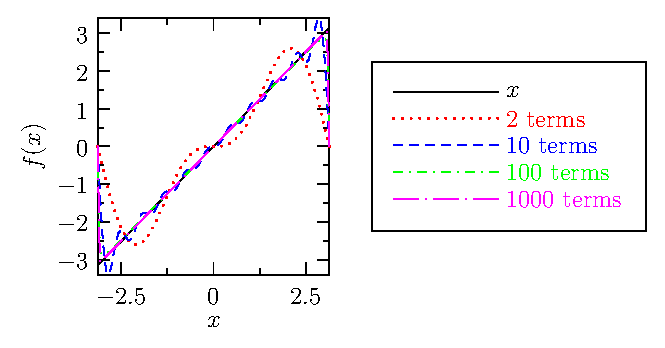
\includegraphics{201/fourierx}
    \caption{Fourier series approximations to $f(x)=x$.}
    \label{fourierx}
  \end{center}
\end{figure}
}

%TODO: something about orthogonality? More examples?

\section{Problems}

\begin{enumerate}
  \item
    What are the Fourier sine and cosine series for
    $y=\sin x$?
    \hidesolution{
      Students should make use of the orthogonality property for $\sin nx$ and
      $\sin mx$, $n \neq m$.
    }
  \item
    What is the Fourier series for $ f(x) = \d(x-1)$?

  \item What is the Fourier series in $x$ for $f(x,t)$ if
    \begin{align}
    f(x,t) =
    \left\{ \begin{array}{ll}
      -t           & \mbox{if $x < 0$};\\
      \phantom{-}t & \mbox{if $x \geq 0$}?
    \end{array} \right.
    \end{align}

\end{enumerate}


\chapter{Partial Differential Equations:
         \\Actually Solving Them}

Let us now return to the heat equation,
\begin{align}
\label{heateq}
\pp{y}{t} = \beta \frac{\partial^2y}{\partial x^2},
\end{align}
and add some \emph{initial conditions}
\begin{align*}
y(x,0)=f(x),
\end{align*}
and \emph{boundary conditions}
\begin{align}
\label{homdibc}
y(0,t)=0, \qquad y(\pi,t)=0.
\end{align}
Physically, this corresponds to modelling the temperature on a rod of length
$2\pi$ in contact at both ends with a heat sink with temperature $0$ (note
that this is not necessarily absolute zero: if we take $y=y+C$, the equation
remains the same, so our base temperature is arbitrary.) The
rod starts with the temperature at position $x$ given by $f(x)$.

We'll solve this using separation of variables:
\begin{align}\label{heatF}
y = \sum_{n=0}^\infty T_n(t) X_n(x),
\end{align}
where we have taken $X_n(x)$ to be orthogonal\footnote{That is, if $n\neq m$,
then $\int_0^\pi X_n(x) X_m(x) dx =0.$ This is the case with elements of
$\{\cos(nx),\sin(nx),n=0,1,\dots \}$.}.
Putting equation \eqref{heatF} into equation \eqref{heateq}, we get
\begin{align}\label{heats}
\sum_{n=0}^\infty \ddt{T_n(t)}X_n(x)
=\beta\sum_{n=0}^\infty T_n(t)\ddtwo{X_n(x)}{x}
\end{align}
Now, since the $X_n$'s are orthogonal, this actually holds term-by-term. That
is, for each $n$, we have
\begin{align*}
T_n'(t)X_n(x) = \beta  T_n(t)X_n''(x)
\quad \implies \quad
\frac{1}{\beta}\frac{T_n'(t)}{T_n(t)}= \frac{X_n''(x)}{X_n(x)}.
\end{align*}
Now, the LHS is independent of $x$, so the RHS must also be independent of $x$.
Since the RHS is also clearly independent of $t$, it must be constant. That is,
\begin{align*}
\frac{1}{\beta}\frac{T_n'(t)}{T_n(t)}= \frac{X_n''(x)}{X_n(x)} = K_n,
\end{align*}
where $K_n$ can only depend on $n$.

This gives us an ODE for $X_n$,
\begin{align}
\label{Eigenfunction}
X_n'' = K_n X_n.
\end{align}
Now, depending on the sign of $K_n$, we have three possibilities, which we will
deal with by enforcing the boundary conditions. Since the $X_n$ are orthogonal,
the boundary conditions must be satisfied for each $n$. The cases are:
\begin{enumerate}
  \item $K_n=k_n^2 > 0$. In this case, $X_n(x)= C_1 e^{k_n x} +C_2 e^{-k_n x}$.
    But then, $X_n(0)=0$ and $X_n(\pi)=0$ imply that $C_1=C_2=0$, so $X_n=0$ in
    this case.
  \item $K_n = 0$. In this case, we get $X_n(x)=Ax +B$. Again, the boundary
    conditions imply that $A=B=0$, so $X_n=0$ in this case.
  \item $K_n =-k_n^2 < 0$. This gives us periodic behaviour,
    \begin{align*}
    X_n(x)=C_1\cos(k_nx) + C_2\sin(k_nx).
    \end{align*}
    We require that $X_n(0)=C_1=0$, so we can remove all the cosines. The
    other boundary condition gives us
    \begin{align*}
    X_n(\pi)=C_2\sin(k_n\pi)=0,
    \end{align*}
    which implies that either $C_2=0$ or $k_n$ is an integer. Since this is
    our last chance to have $X_n$ not be zero everywhere, we can't have $C_2=0$,
    so we set $k_n$ to be an integer. In particular, set $k_n=n$.
\end{enumerate}
Thus, $K_n=-n^2$, and $X_n= \sin(nx)$. Much simpler!

We now have enough information to start determining $T_n$. We know that
$K_n=-n^2$, so $T_n$ obeys the equation
\begin{align*}
T_n' = \beta K_n T_n = - \beta n^2 T_n
\qquad \implies \qquad
T_n = T_n(0) e^{-\beta n^2 t}.
\end{align*}

Putting this together, our solution (so far) is
\begin{align*}
y(x,t) = \sum_{n=0}^\infty T_n(0) e^{-\beta n^2 t} \sin(nx).
\end{align*}
To get this, we have used the original equation and the boundary conditions.
We still have to determine the values of $T_n(0)$, for which we will use the
initial conditions, $y(x,0)=f(x)$. That is,
\begin{align*}
y(x,0)=f(x) =  \sum_{n=0}^\infty T_n(0) e^{-\beta n^2 t} \sin(nx)
= \sum_{n=0}^\infty T_n(0) \sin(nx).
\end{align*}
In other words, this is just a sine-series for $f(x)$! However, instead of
integrating over $(-\pi,\pi)$, we only know $f(x)$ for $x\in(0,\pi)$. We can
solve this problem by extending $f(x)$ as an odd function by setting
$f(-x)=-f(x)$, so the coefficients are given by
\begin{align*}
T_n(0)=\frac{1}{\pi}\int_{-\pi}^\pi f(x)\sin(nx)dx
=\frac{2}{\pi}\int_0^\pi f(x)\sin(nx)dx,
\end{align*}
since the integrand is even.

The solution to the heat equation is then
\begin{align}
\boxed{
y(x,t)=\frac{2}{\pi}
\sum_{n=1}^\infty \[\int_0^\pi f(x)\sin(nx)\,dx\]
e^{-kn^2t}
\sin(nx)}.
\end{align}

\oexample{
  The initial temperature in a rod of length $\pi$ is given by
  \begin{align}
  \label{heat1ic}
  y(x,0)=2\sin(x)+\sin(5x),
  \end{align}
  and the temperature at the ends of the rod is kept at zero. Assuming that
  \begin{align*}
  \pp{y}{t} = \beta \frac{\partial^2 y}{\partial x^2},
  \end{align*}
  find $y(x,t)$ for $x\in(0,\pi)$, $t>0$.
  }{
  The boundary conditions match those given in equation \eqref{homdibc}, so
  the above analysis shows that we can express $y$ as a linear combination
  of $\{\sin(nx),n=1,2,\dots\}$. That is,
  \begin{align*}
  y(x,t)=\sum_{n=1}^\infty T_n(0) e^{-\b n^2 t} \sin(nx).
  \end{align*}
  The initial conditions are that $y(x,0)=2\sin(x)+\sin(5x)$, so $T_1(0)=2$,
  $T_5(0)=1$, and all others are zero. We can then write the solution as
  \begin{align*}
  y(x,t) = 2 e^{-\b t} \sin(x) + e^{-25 \b t} \sin(5x).
  \end{align*}
%FIXME: Is this enough explanation?
 This result is shown for various times in figure \ref{heat1} for $\b=1$.
  \begin{figure}[htbp]
    \begin{center}
      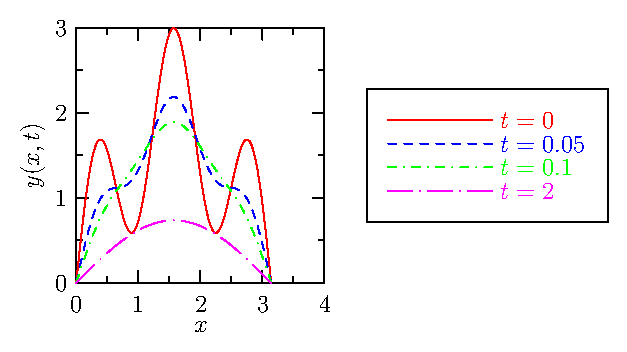
\includegraphics{201/heat1}
      \caption{The temperature at different times with initial conditions
        given in \eqref{heat1ic}. Notice that the $\sin(5x)$ term, which
        decays like $e^{-25 \b t}$, is relevant only for small $t$. }
      \label{heat1}
    \end{center}
  \end{figure}
}


\section{Non-homogeneous constant boundary conditions}

Suppose that the boundary conditions were instead
\begin{align*}
y(0,t)=A, \qquad y(\pi,t)=B.
\end{align*}
Notice that these conditions match the case $K_n=0$ with
\begin{align*}
y(x,t)=\frac{B-A}{\pi}x+A.
\end{align*}
This obeys the heat equation, since
\begin{align*}
\frac{\partial^2}{\partial x^2}(mx+b)=0= \pp{}{t}(mx+b),
\end{align*}
and is independent of $t$, i.e.\ it is a steady state solution. Then, setting
\begin{align*}
g(x) = f(x) - \(A+ \frac{B-A}{\pi}x\),
\end{align*}
\begin{align}
\label{diribc}
y(x,t)=A + \frac{B-A}{\pi}x +
\frac{2}{\pi}
\sum_{n=1}^\infty\(\int_{0}^\pi g(x)\sin(nx)dx\) e^{-\b n^2t} \sin(nx)
\end{align}
matches both the initial and boundary conditions.

\oexample{
  Solve the initial boundary problem
  \begin{align*}
  \label{heat3ic}
  \pp{y}{t} = \b \pptwo{y}{x}, \qquad y(0)=1, \quad y(\pi)=1+\pi,
  \quad y(x,0)=f(x)=x^2 +x +1
  \end{align*}
  for $y(x,t)$.

}{
  The steady-state solution is $x+1$. Let
  \begin{align*}
  g(x) = f(x) -(x+1) = x^2
  \end{align*}
  Then,
  \begin{align*}
  y(x,t) = 1 + x + \sum_{n=1}^\infty T_n(0) e^{-\b n^2 t} \sin(nx).
  \end{align*}
  And in order to satisfy $y(x,0)=1+x+x^2$, we have
  \begin{align*}
  x^2 = \sum_{n=1}^\infty T_n(0) \sin(nx).
  \end{align*}
  The coefficients are given by the formula
  \begin{align*}
  T_n(0) &=& \frac{2}{\pi} \int_0^\pi x^2 \sin(nx) \, dx
  \\\nonumber
  &=& \frac{2}{\pi}\[\left.x^2 \frac{-\cos(nx)}{n} \right|_0^\pi
  + \frac{2}{n}\int_0^\pi x \cos(nx)dx\]
  \\\nonumber
  &=& \frac{2}{n\pi}\[ -\pi^2\cos(n\pi)+2(\left.\frac{x \sin(nx)}{n}
  \right|_0^\pi
  - \frac{1}{n}\int_0^\pi\sin(nx)dx)  \]
  \\\nonumber
  &=& \frac{-2\pi}{n}\cos(n\pi)-\frac{4}{n^3\pi} \left.-\cos(nx) \right|_0^\pi
  = \frac{-2\pi}{n}(-1)^n + \frac{4(\(-1)^n-1\)}{n^3\pi}
  \end{align*}
  The solution is therefore
  \begin{align*}
  y(x,t) = 1+x+
  \sum_{n=1}^\infty \[\frac{-2\pi}{n}(-1)^n + \frac{4(\(-1)^n-1\)}{n^3\pi}\]
  e^{-\b n^2 t}\sin(nx).
  \end{align*}
% Useless figure
%  as can be seen in figure \ref{heat3}. \qed
%  \begin{figure}[htbp]
%    \begin{center}
%      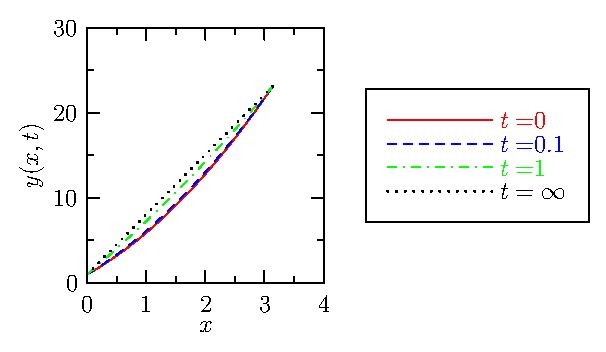
\includegraphics{201/heat3}
%      \caption{The temperature at different times for the system given in
%        \eqref{heat3ic}.}
%      \label{heat3}
%    \end{center}
%  \end{figure}

}
% This lab is too long!
%\section{A more complicated example}
%
%\oexample{
%  The heat in a rod obey the equation
%  \begin{align}
%  \pp{y}{t}=\pptwo{y}{x}.
%  \end{align}
%  Given the boundary conditions
%  \begin{align}
%  \label{heat2ic}
%  y(0,t)=1 \qquad y(\pi,t)=e^\pi
%  \end{align}
%  and the and the initial condition $y(x,0)=e^x$, find $y(x,t)$.\\
%}{
%  The solution is given by
%  \begin{align}
%  y(x,t)&=&1 + \frac{e^\pi-1}{\pi}x +
%  \sum_{n=1}^\infty T_n(0) e^{-n^2t} \sin(nx),
%  \\
%  T_n(0)&=&\frac{2}{\pi}\int_{0}^\pi g(x)\sin(nx)dx,
%  \\
%  g(x)&=&e^x - 1 - \frac{e^\pi-1}{\pi}x.
%  \end{align}
%  From equation \eqref{Fourierx}, we have
%  \begin{align}
%  x = 2 \sum_{n=1}^\infty  \frac{(-1)^{n+1}}{n} \sin(nx)
%  \end{align}
%  To find the Fourier sine-series for $e^x$, we must compute
%  \begin{align}
%  a_n = \frac{2}{\pi}\int_0^\pi e^x \sin(nx) \, dx
%  = \frac{2}{\pi}\left.\frac{e^x\(\sin(nu) - n \cos(nu)\)}{n^2+1}\right|_0^\pi
%  = \frac{2}{\pi}\frac{n(1 - (-1)^ne^\pi)}{n^2+1}
%  \end{align}
%  Also, the Fourier series for $1$ over $x\in(-\pi,\pi)$ has coefficients
%  \begin{align}
%  \frac{2}{\pi}\int_0^\pi \sin(nx) = \frac{2}{n\pi}\left.\cos(nx) \right|_0^\pi
%  = \frac{2\((-1^n)-1\)}{n\pi},
%  \end{align}
%  so, over $x\in(0,\pi)$,
%  \begin{align}
%  1 = \sum_{n=1}^\infty \frac{2\((-1^n)-1\)}{n\pi} \sin(nx).
%  \end{align}
%
%  Noting that the Fourier series is a linear, so we can add the series
%  together:
%  \begin{align}
%  e^x - 1- \frac{e^\pi}{\pi}x
%  &=& \sum_{n=1}^\infty \frac{2}{\pi}n\frac{1 - (-1)^ne^\pi}{n^2+1} \sin(nx)
%  - \frac{e^\pi-1}{\pi} 2 \sum_{n=1}^\infty  \frac{(-1)^{n+1}}{n} \sin(nx)
%  \\ \nonumber
%  &&-\sum_{n=1}^\infty \frac{2\((-1^n)-1\)}{n\pi} \sin(nx)
%  \\ \nonumber
%  &=&\sum_{n=1}^\infty \(\frac{2}{\pi}\frac{n(1 - (-1)^ne^\pi)}{n^2+1}
%  -\frac{e^\pi-1}{\pi}2 \frac{(-1)^{n+1}}{n}- \frac{2\((-1^n)-1\)}{n\pi}\)
%  \sin(nx).
%  \end{align}
%  Now, this is all a bit messy, but we do end up with the solution
%  \begin{align}
%  y(x,t) = 1 &+& \frac{e^\pi-1}{\pi}x
%  \\ \nonumber
%  &+&
%  \sum_{n=1}^\infty \(\frac{2}{\pi}\frac{n(1 - (-1)^ne^\pi)}{n^2+1}
%  -2 \frac{e^\pi-1}{\pi} \frac{(-1)^{n+1}}{n}- \frac{2\((-1^n)-1\)}{n\pi}\)
%    e^{-n^2t} \sin(nx),
%  \end{align}
%  as can be seen in figure \ref{heat2}. \qed
%  \begin{figure}[htbp]
%    \begin{center}
%      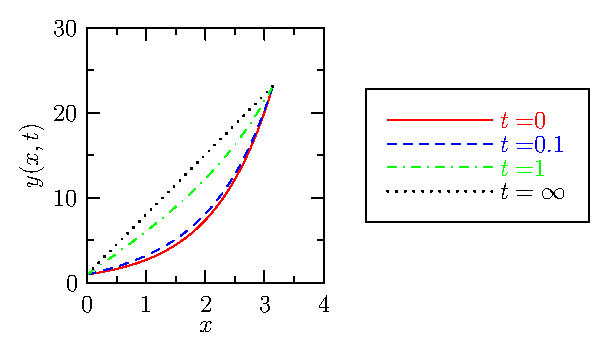
\includegraphics{201/heat2}
%      \caption{The temperature at different times with initial conditions
%        given in \eqref{heat2ic}.}
%      \label{heat2}
%    \end{center}
%  \end{figure}
%}



\section{Problems}

\begin{enumerate}
  \item
    Show that equation \eqref{diribc} does indeed solve the heat equation
    with the given boundary and initial conditions.
  \item
    An inanimate carbon rod of length $\pi$ is hit with a ``laser'',
    transferring an amount of heat $H$ to a point at its centre. That is, the
    initial temperature distribution along its length is given by
    \begin{align*}
    y(x,0)=H\delta\(x-\frac{\pi}{2}\).
    \end{align*}
    If the ends of the rod are kept at constant temperature $0$, and the
    temperature in the rod obeys the relationship
    \begin{align*}
    \pp{y}{t} = \beta \frac{\partial^2 y}{\partial x^2},
    \end{align*}
    find $y(x,t)$ for all $t\geq 0$.
    \hidesolution{
      Following the above procedure,
      \begin{align*}
      y(x,t)=\frac{2}{\pi}
      \sum_{n=1}^\infty T_n(0) e^{-kn^2t} \sin(nx)
      \end{align*}
      with
      \begin{align*}
      T_n(0) &=& \frac{2}{\pi}\int_0^\pi H \d\(x-\frac{\pi}{2} \) \sin(nx) \, dx
      \\
      &=& \frac{2H}{\pi} \sin\(\frac{n\pi}{2}\)
      \\
      &=& \frac{2H}{\pi}
      \left\{ \begin{array}{ll}
        0,           & \mbox{if $n=2m$}\\
        \sin\(m\pi+ \frac{\pi}{2}\), & \mbox{if $n=2m+1$}
      \end{array} \right.
      \\
      &=& \frac{2H}{\pi}
      \left\{ \begin{array}{ll}
        0,           & \mbox{if $n=2m$}\\
        (-1)^m, & \mbox{if $n=2m+1$}.
      \end{array} \right.
      \end{align*}
      The solution is then given by
      \begin{align*}
      y(x,t) = \frac{2H}{\pi} \sum_{m=0}^\infty (-1)^m e^{-4\beta m^2 t} \sin(2mx)
      \end{align*}
    }
  \item
    \emph{Neumann boundary conditions} specify the value of the function at
    the boundary, e.g. $y(0,t)=A$, $y(\pi,t)=B$ with $A$ and $B$ constant.
    We showed that the set of Eigenfunctions given by equation
    \eqref{Eigenfunction} must be $\{\sin(nx),n=1,2,\dots\}$ in this case.
    If the boundary conditions were instead \emph{Dirichlet boundary conditions}
    such as
    \begin{align*}
    \left.\pp{y(x,t)}{x}\right|_{x=0}=0, \qquad
        \left.\pp{y(x,t)}{x}\right|_{x=\pi}=0,
    \end{align*}
    what are the Eigenfunctions?


\end{enumerate}


\chapter{Tables}

\section{Table of Integrals}

\begin{align}\nonumber
&\int u dv = uv - \int v du
&
\\\nonumber
& \int \cos x dx = -\sin x
& \int \sin x dx = \cos x
\\\nonumber
& \int \tan x dx  = -\ln\abs{\cos x}
&
\\\nonumber
& \int \sin^2 x dx = \frac{1}{2}x - \frac{1}{4}\sin 2x
& \int \cos^2 x dx = \frac{1}{2}x + \frac{1}{4}\sin 2x
\\\nonumber
& \int \tan^2 x dx  = \tan x - x
&
\\\nonumber
& \int \sin^n x dx = -\frac{\sin^{n-1}x\cos{x}}{n}
+ \frac{n-1}{n}\int\sin^{n-2}xdx
&
\\\nonumber
& \int \cos^n x dx = \frac{\cos^{n-1}x\sin x}{n}
+ \frac{n-1}{n}\int \cos^{n-2}x dx
&
\\\nonumber
& \int \sin ax \sin bx dx = - \frac{\sin(a+b)x}{2(a+b)}
  + \frac{\sin(a-b)x}{2(a-b)},\quad a^2\neq b^2
&
\\\nonumber
& \int \cos ax \cos bx dx = \frac{\sin(a+b)x}{2(a+b)}
+ \frac{\sin(a-b)x}{2(a-b)},\quad a^2\neq b^2
&
\\\nonumber
& \int \sin ax \cos bx dx = -\frac{\cos(a+b)x}{2(a+b)}
- \frac{\cos(a-b)x}{2(a-b)},\quad a^2\neq b^2
&
\\\nonumber
& \int \sec^2 x dx = \tan x
& \int \csc^2 x dx = -\cot x
\\\nonumber
& \int \sec x \tan x  dx = \sec x
&
\\\nonumber
& \int \frac{dx}{\sqrt{a^2-x^2}}= \arcsin\frac{x}{a}
& \int \frac{dx}{x\sqrt{x^2-a^2}}= \frac{1}{a}\arccos\frac{a}{x}
\\\nonumber
&\int \frac{dx}{a^2+x^2} = \frac{1}{a}\arctan\frac{x}{a},
&
\\\nonumber
& \int \frac{dx}{a^2-x^2} = \frac{1}{2a}\ln\abs{\frac{x+a}{x-a}},
& \int \frac{dx}{\sqrt{a^2+x^2}} = \ln\abs{x+\sqrt{x^2+a^2}}
\\\nonumber
& \int \sinh x dx = \cosh x
& \int \cosh x dx = \sinh x
\\\nonumber
& \int e^{ax}\sin nx dx = \frac{e^{ax}\(a \sin nx - n \cos nx \) }{a^2+n^2 }&
\\\nonumber
& \int e^{ax}\cos nx dx = \frac{e^{ax}\(a \cos nx + n \sin nx \) }{a^2+n^2 }
&
\end{align}

\section{Table of Laplace Transforms}

\label{tableolap}
\begin{center}
\begin{tabular}{ l |  l }
  $f(t)$ & $\mathcal{L}(f) = F(s)$  \\
  \hline
  $f'(t)$ & $sF(s) -f(0)$\\
  $f''(t)$ & $s^2F(s) -sf(0) - f'(0)$\\
  $f^{(n)}(t)$ & $s^nF(s) -s^{n-1}f(0)-\dots - f^{(n-1)}(0)$\\
  $t$ & $\frac{1}{s}$ \\
  $t^n$ & $\frac{n!}{s^{n+1}}$ \\
  $e^{\a t}$ & $\frac{1}{s-\a} $ \\
  $e^{\a t}f(t) $ & $F(s-\a) $ \\
  $f(ct) $ & $\frac{1}{c}F\(\frac{s}{c}\) $ \\
  $\sin(\beta t)$ & $\frac{\beta}{s^2 + \beta^2} $ \\
  $\cos(\beta t)$ & $\frac{s}{s^2 + \beta^2} $ \\
  $\sinh(\beta t)$ & $\frac{\beta}{s^2 - \beta^2} $ \\
  $\cosh(\beta t)$ & $\frac{s}{s^2 - \beta^2} $ \\
  $e^{\alpha t}\sin(\beta t)$ & $\frac{\beta}{(s-\alpha)^2 + \beta^2} $ \\
  $e^{\alpha t}\cos(\beta t)$ & $\frac{s-\alpha}{(s-\alpha)^2 + \beta^2} $ \\
  $u_c(t)$ & $\frac{e^{-cs}}{s}$ \\
  $u_c(t)f(t-c)$ & $e^{-cs}F(s)$ \\
  $\delta(t)$ & $1$ \\
  $\int_0^t f(t-\tau) g(\tau) \,d\tau \doteq f*g$ & $F(s)G(s) $ \\
  $f(t)$ with $f(t+T)=f(t)$ & $\frac{\int_0^Tf(t) e^{-st}dt}{1-e^{-sT}}$\\
  $t^n f(t)$ & $(-1)^n \frac{d^n}{ds^n} F(s)$\\
\end{tabular}\\
\end{center}


\section{Table of Taylor Series}
\begin{align}\nonumber
& f(x) = f(a) + f'(a)(x-a) + \frac{f''(a)}{2!} + \dots
+ \frac{f^{(n)}(a)}{n!}(x-a)^n + \dots
%&
%&
\\\nonumber
& e^x = \sum_{n=0}^\infty \frac{x^n}{n!}
\qquad \sin x = \sum_{n=0}^\infty \frac{(-1)^n x^{2n+1}}{(2n+1)!}
\qquad \sin x = \sum_{n=0}^\infty \frac{(-1)^n x^{2n+1}}{(2n+1)!}
\\\nonumber
&\tan x = x + \frac{1}{3}x^3 + \frac{2}{15}x^5 + \frac{17}{315}x^7
+ \frac{62}{2835}x^9 + \dots
\\\nonumber
&\arcsin x = x + \frac{1}{2}\frac{x^3}{3}
+ \frac{1\cdot 3}{2\cdot 4}\frac{x^5}{5}
+ \frac{1\cdot3\cdot5}{2\cdot4\cdot6}\frac{x^7}{7} + \dots
\\\nonumber
&\arctan x = \sum_{n=0}^\infty (-1)^n \frac{x^{2n+1}}{2n+1}
\\\nonumber
&\frac{1}{1-x} = \sum_{n=0}^\infty x^n
\qquad \ln(1-x) = -\sum_{n=1}^\infty \frac{x^n}{n}
\end{align}



\chapter{Second-order Linear Equations}
% Text chapter 4.2
Let $a,b,c$ be real numbers. Second order equations of the form
\begin{dmath}
  \label{sec2hom}
  a \ddtwo{y}{t} + b \dd{y}{t} + cy =0
\end{dmath}
are linear in $y$. If both $y_1$ and $y_2$ are solutions to
equation (\ref{sec2hom}), and $\alpha$ and $\beta$ are constants, then
%\newcommand\alpha y_1 + \beta y_2{\alpha y_1 + \beta y_2}
\begin{align*}
&& a \ddtwo{\(\alpha y_1 + \beta y_2\)}{t} + b \dd{\(\alpha y_1 + \beta y_2\)}{t} + c \(\alpha y_1 + \beta y_2 \)
\\  \nonumber
&&= \alpha\(a \ddtwo{y_1}{t} + b \dd{y_1}{t} + cy_1 \)
+\beta\(a \ddtwo{y_2}{t} + b \dd{y_2}{t} + cy_2 \)
\\ \nonumber
&&= \alpha \(0\) +\beta \(0\) =0,
\end{align*}
In other words, $\alpha y_1 + \beta y_2$, which is a linear combination of $y_1$ and $y_2$, is
also a solution to equation (\ref{sec2hom}). Being able to use this linearity
is a powerful tool that we can use to solve this very important type of
differential equation. We will, in general, have two solutions to these
second-order differential equations, and we will need two initial values to
fully determine the solution. This is expressed in the following theorem:

\begin{theorem}
  Let $b$, $c$, $Y_0$, and $Y_1 \in \mathbb{R}$.
  Then, the initial value problem
  \begin{align*}
  y'' + by' + cy =0, \qquad y(0)=Y_0, \quad y'(0)=Y_1
  \end{align*}
  has a unique solution.
\end{theorem}

\section{Homogeneous Linear Equations}
The behaviour of these systems is basically exponential. To see this,
set $y=e^{rt}$. Then, putting this into equation (\ref{sec2hom}), we get
\begin{align*}
a r^2 e^{rt} + b r e^{rt} + ce^{rt}
= e^{rt} \( ar^2 + br + c\) =0.
\end{align*}
Since $e^{rt}$ is never zero, there is no harm in dividing by it. This leaves
us with the \emph{characteristic equation},
\begin{dmath}
  \boxed{ar^2 + br + c =0},
\end{dmath}
which allows us to determine $r$ using the quadratic formula. In this way
we get two solutions,
\begin{align*}
\boxed{y_1=e^{r_1 t}\text{ and }y_2=e^{r_2 t}},
\end{align*}
from the two solutions $r_1$ and $r_2$ of the characteristic equation.\\

\noindent\emph{Example}: Solve the second-order homogeneous equation
\begin{align*}
\ddtwo{y}{t} - y =0,
\end{align*}
with initial conditions $y(0) =1, \, y'(0) =0.$\\
\noindent\emph{Solution}:
Setting $y=e^{rt}$, this becomes
\begin{align*}
e^{rt} \(r^2 -1 \) = e^{rt} \(r-1\)\(r+1\) =0,
\end{align*}
so $r_1=-1$, and $r_2=1$. Thus,
\begin{align*}
y_1(t) = e^{-t}, \qquad y_2(t) =e^t.
\end{align*}
The solution $y$ is therefore a linear combination of $y_1$ and $y_2$. That is,
\begin{align*}
y(t) = \alpha y_1(t) + \beta y_2(t) = \alpha e^{-t} + \beta e^t,
\end{align*}
for some constants $\alpha$ and $\beta$ that are determined by the initial
conditions. Since $y(0)=1$,
\begin{dmath}
  \label{sec2ab1}
  y(0) = \alpha +\beta =1.
\end{dmath}
Since $y'(0)=0$, and $y'(t) = -\alpha e^{-t} + \beta e^t$,
\begin{dmath}
  \label{sec2ab2}
  y'(0) = -\alpha + \beta =0.
\end{dmath}
Combining equations \eqref{sec2ab1} and \eqref{sec2ab2}, it is easy to see
that $\alpha = \beta =\half$. The solution is therefore
\begin{align*}
y = \frac{e^{-t} + e^t}{2}. \qed
\end{align*}

\section{Dealing with complex roots}
%Text section 4.3
So far, we've seen only problems where the roots of the characteristic
equation are real. Of course, this isn't always the case, but we can deal with
this using \emph{Euler's Formula},
\begin{align*}
\boxed{e^{i\theta} = \cos(\theta) + i \sin(\theta)}.
\end{align*}
For example, if we get $r_{1,2}= 4\pm 2i$, then solutions are a linear
combination of
\begin{align*}
e^{(4+2i)t}=e^{4t}e^{i2t}=e^{4t} \(\cos(2t) + i \sin(2t)\)
\end{align*}
and
\begin{align*}
e^{(4-2i)t}=e^{4t}e^{-i2t}=e^{4t} \(\cos(2t) - i \sin(2t)\).
\end{align*}
An easy way to get all linear combinations is to just set
\begin{align*}
y_1(t) = e^{4t} \cos(2t), \qquad y_2(t) = e^{4t} \sin(2t).
\end{align*}
\\

\noindent\emph{Example}: Give the general solution to
\begin{align*}
\ddtwo{y}{t} + 1 =0
\end{align*}
with initial conditions $y(0) =1, \, y'(0) =0.$\\
\noindent\emph{Solution}:
The characteristic equation is
\begin{align*}
r^2 +1 =0 \quad \implies \quad r = \pm i.
\end{align*}
The solution is then a linear combination of
\begin{align*}
y_1(t) = e^{0t}\cos(t) = \cos(t), \qquad
y_2(t) = e^{0t}\sin(t) = \sin(t)
\end{align*}
Setting $y(t)=\alpha \cos(t) + \beta \sin(t)$, we can input the initial
conditions to get
\begin{dmath*}[compact]
  y(0) = \alpha\cos(0) + \beta\sin(0) = \alpha =1, \qquad
  y'(0) = -\alpha\sin(0) + \beta\cos(0) =\beta =0.
\end{dmath*}
The solution to the IVP is then $y(t) = \cos(t)$. \qed 

\section{Dealing with repeated roots}
In the above section, we were lucky, since we had two independent roots.
Two independent roots gave two independent solutions $y_1$ and $y_2$, which
we used to solve the two initial values for the problem. When we have
repeated roots, we still need to make sure that we have two independent
solutions. How do we get this? Well, just multiply one solution by $t$.
% TODO: add a footnote as to why this makes sense.

For example, suppose that we solved the characteristic equation and got
$r_1=r_2=r$. We still get one solution out of this, namely
\begin{align*}
y_1(t) =e^{rt}.
\end{align*}
To get the second solution, just take
\begin{align*}
y_2(t) = t y_1(t) = t e^{rt}.
\end{align*}
This works since $\ddtwo{t}{t}=0$, so the extra $t$ in $y_2$ is eventually
killed, and everything cancels out nicely.
\\

\noindent\emph{Example}: Give the general solution to
\begin{align*}
\ddtwo{y}{t} - 2 \dd{y}{t}+1 =0
\end{align*}
with initial conditions $y(0) =1, \, y'(0) =0.$\\
\noindent\emph{Solution}:
The characteristic equation for this problem is
\begin{align*}
r^2 - 2r +1 = (r-1)(r-1) =0,
\end{align*}
which has the double root $r_1=r_2=1$. Thus, set
$y_1(t) = e^t$ and $y_2=t e^t$, so
\begin{align*}
y = \alpha e^t + \beta t e^t
\end{align*}
Now,
\begin{align*}
y(0) = \alpha = 1.
\end{align*}
For the second condition, calculate that
$y'(t) = \alpha e^t + \beta e^t + \beta te^t$. Thus
\begin{align*}
y'(0) = \alpha + \beta =0.
\end{align*}
Thus, $\alpha=1$ and $\beta =-1$, so the solution is
\begin{align*}
y(t) = e^t - te^t. \qed
\end{align*}


\section{Problems}

\begin{enumerate}

\item
  % Real roots
  Solve the IVP
  \begin{align*}
  2 y'' + 5y' + 2y =0
  \end{align*}
  with initial conditions $y(0)=0$ and $y'(0)=3/2$.

\item
  Solve the IVP
  % imaginary roots
  \begin{align*}
  2 y'' + 8y =0
  \end{align*}
  with initial conditions $y(0)=1$ and $y'(0)=2$.

\item
  Solve the IVP
  % complex roots
  \begin{align*}
  y'' + 2y' + 4y=0
  \end{align*}
  with initial conditions $y(0)=0$ and $y'(0)=2$.
  %r = -1 \pm i \sqrt{3}
  % y =2 \sqrt{3} e^{-t} \sin(\sqrt{3}t\)

\item
  Prove Euler's formula using differential equations. \\
  Consider the IVP
  \begin{align*}
  y'' +y =0, \qquad y(0)=1, \quad y'(0)=i.
  \end{align*}
  \begin{enumerate}
    \item Step 1: Show that $\{y_1=\cos(t),y_2=\sin(t)\}$ are solutions
      to the differential equation. Find a solution $y=\alpha y_1 + \beta y_2$
      to the IVP.
    \item Step 2: Using the characteristic equation, find a different pair
      of solutions $\{y_1,y_2\}$ made up of complex exponentials. Find a
      solution $y=\alpha y_1 + \beta y_2$ to the IVP.
    \item Step 3: Use a theorem to show that these two solutions must be
      identical, thereby proving Euler's formula.
  \end{enumerate}

\item
  % Mazowita's question. Solution is tex'd.
  Find the general solution of the differential equation
  \begin{align*}
  10, \! 000 \, y'' - 100, \! 000 \, y' + 250, \! 000 \, y = 0.
  \end{align*}


\item
  % Mazowita's question. Solution is tex'd.
  Solve the IVP
  \begin{align*}
  y'' + 4y' + 5y = 0
  \end{align*}
  with $y(\pi) =\ e^{-\pi},$ $y' (0) = \sqrt{\pi} + 2e^\pi$.

\end{enumerate}


\chapter{Non-homogeneous Second-Order Linear Equations}

\section{Method of Undetermined Coefficients}
% Text section  4.4
The next step is to add a function to the right-hand side of equation
(\ref{sec2hom}), so that we get
\begin{align*}
a y'' + b y' + cy =f(t).
\end{align*}
Then what we have is a \emph{non-homogeneous equation} and we say that equation
$a y'' + b y' + cy =0$ is the corresponding homogeneous equation.

In this section, we are going to restrict ourselves to a couple of choices
for $f(t)$ so that we can use the method of \emph{undetermined coefficients},
also known as \emph{we can probably guess what the answer is, so let's do
that}.

The idea behind this method is trying to find the particular solution $y_p$,
which has the property
\begin{dmath}
  \label{yp}
  a y_p'' + b y_p' + cy_p =f(t),
\end{dmath}
though it need not match the initial conditions. For instance, if
$f(t)=\sin(t)$, guessing that $y_p = A \sin(t) + B \cos(t)$ would probably do
the trick. We can just substitute $y_p = A \sin(t) + B \cos(t)$ into equation
\eqref{yp} in order to find the values of $A$ and $B$ that work.

Here is a table that will guide you, young jedi:
\begin{align*}
\begin{tabular}{ l |  l }
  $f(t)$ & $y_p$  \\
  \hline
  $ke^{at}$ & $Ce^{at}$  \\
  $kt^n$ & $C_n t^n + C_{n-1}t^{n-1} + \dots + C_1 t + C_0 $  \\
  $k \cos(at)$ or $k \sin(at)$ & $K \cos(at) + M\sin(at)$ \\
  $kt^n e^{at}$ & $e^{at}\(C_n t^n + C_{n-1}t^{n-1} + \dots + C_1 t + C_0\)$ \\
  $k t^n \cos(at)$ or $k t^n \sin(at)$ &
  $\(C_nt^n + \dots +C_0 \)\cos(at) + \(D_nt^n + \dots + D_0 \)\sin(at)$ \\
  $ke^{at} \cos(bt)$ or $ke^{at} \sin(bt)$ &
  $e^{at}\(K \cos(at) + M\sin(at)\)$ \\
  $k t^n e^{at }\cos(bt)$ or $k t^n e^{at} \sin(bt)$ &
  $\(C_nt^n + \dots +C_0 \)e^{at}\cos(bt)
  + \(D_nt^n + \dots + D_0 \)e^{bt}\sin(bt)$ \\
\end{tabular}
\end{align*}
Finally, if your guess ends up being a polynomial times a linear
combination of the solutions to the corresponding homogeneous equation (known
as $y_1$ and $y_2$ in previous lab), then multiply your
guess by $t$ until it isn't. For example, if $y_1=e^t$, $y_2=e^{2t}$, and
$f(t)=t^2e^t$, then you would choose $y_p = t\(C_2 t^2 + C_1 t + C_0 \)e^t$.
If $y_1=e^t$, $y_2=t e^t$, and $f(t)=t^2e^t$, then you would choose
$y_p = t^2 \(C_2 t^2 + C_1 t + C_0 \)e^t$.

Once you have determined $y_p$, combine it with the homogeneous solutions
to give the general solution
\begin{dmath}
  \boxed{y(t) = \alpha y_1(t) + \beta y_2(t) + y_p(t) }
\end{dmath}
to match the initial conditions.
\\

\noindent \emph{Example}:
Solve the IVP
\begin{dmath}
  \label{undetceg}
  y'' -3y' +2 y = t
\end{dmath}
with $y(0) = 3/4$ and $y'(0) = 3/2$.\\
\noindent \emph{Solution}:
This has characteristic equation
\begin{align*}
r^2 -3r +2 = (r-1)(r-2) \quad \implies \quad r_1=1, \, r_2=2,
\end{align*}
so the homogeneous solutions are $y_1(t) = e^t, \, y_2=e^{2t}$. Since
$f(t)=t$ is not a linear combination of $y_1$ and $y_2$, we can just choose
$y_p = C_1 t + C_0$. Putting this into equation \eqref{undetceg}, we get
\begin{align*}
\ddtwo{(C_1 t + C_0)}{t} -3\dd{(C_1 t + C_0)}{t} + 2 \(C_1 t + C_0\) =t
\quad \implies \quad
-3 C_1 + 2C_1 t + 2C_0 = t,
\end{align*}
so $C_1=1/2$ and $C_0=3/4$. Thus, $y_p = \frac{t}{2} +\frac{3}{4}$, and the
general solution is
\begin{align*}
y = \alpha e^t + \beta e^{2t} + \frac{t}{2} +\frac{3}{4}.
\end{align*}
Now, we satisfy the initial conditions:
\begin{align*}
y(0) = \alpha + \beta +\frac{3}{4} = \frac{3}{4}
\quad \implies \quad \alpha+\beta=0,
\end{align*}
and
\begin{align*}
y'(0) = \alpha + 2\beta + \half = \frac{3}{2}
\quad \implies \quad \alpha+2 \beta=1
\end{align*}
so $\alpha=-1$ and $\beta =1$. The solution is therefore
\begin{align*}
y(t) = -e^t +e^{2t}  + \frac{t}{2} +\frac{3}{4}.
\end{align*}
Let's check this solution. We have
\begin{eqnarray*}
  y(t) &=& -e^t +e^{2t}  + \frac{t}{2} +\frac{3}{4} \\
  y'(t) &=& -e^t +2e^{2t}  + \frac{1}{2}\\
  y''(t) &=& -e^t +4 e^{2t}.
\end{eqnarray*}
Putting these into equation \eqref{undetceg} yields
\begin{align*}
&&y'' - 3 y' + 2 y
\\
&&= \(-e^t + 4 e^{2t}\)
-3 \(-e^t +2e^{2t}  + \frac{1}{2} \)
+2 \(-e^t +e^{2t}  + \frac{t}{2} + \frac{3}{4} \) = t,
\end{align*}
as required. \qed

\section{Superposition Principle}
Suppose that we know the solution $y_{1,p}$ to
\begin{dmath}
  ay'' + by' + cy = f(t)
\end{dmath}
and the solution $y_{2,p}$ to
\begin{dmath}
  ay'' + by' + cy = g(t).
\end{dmath}
We can use these to determine the solution to the more difficult problem
\begin{dmath}
  \label{super}
  ay'' + by' +cy = A f(t) + B g(t)
\end{dmath}
by using the fact that the differential operator
\begin{dmath}
  L = a \ddtwo{}{t}  + b \dd{}{t} + c
\end{dmath}
is linear. That is, for constants $\alpha$ and $\beta$
\begin{align}
  L\(\alpha y_{1,p} + \beta y_{2,p} \)
  &=
  a \(\alpha y_{1,p} + \beta y_{2,p} \)'' + b \(\alpha y_{1,p}+\beta y_{2,p}\)'
  + c\(\alpha y_{1,p} + \beta y_{2,p} \)
  \\
  &= \alpha \(a y_{1,p}'' + b y_{1,p}' + c  y_{1,p}\)
  + \beta \(a y_{2,p}'' + b y_{2,p}' + c  y_{2,p}\)
  \\
  &=
  \alpha L\( y_{1,p}\)  + \beta L\(y_{2,p} \),
\end{align}
just like ``linearity'' is defined in linear algebra. Then since
$L\(y_{1,p}\)= f(t)$ and $L\(y_{2,p}\) = g(t)$,
\begin{dmath}
  L\(A y_{1,p} + B y_{2,p} \) = A f(t) + B g(t),
\end{dmath}
which gives us the particular solution for equation \eqref{super} without
having to do a lot of extra work.
\\

\noindent\emph{Example}: Find the general solution to
\begin{dmath}
  y'' -3 y' -4y = t + 10 e^{-t}.
\end{dmath}
\noindent\emph{Solution}:
The characteristic equation for the homogeneous part is
$0 = r^2 -3r -4 = (r+1)(r-4)$ which gives $r_1=-1$ and $r_2=4$. The solution
space is then spanned by $\{y_1=e^{-t},y_2=e^{4t}\}$.
We can use the superposition principle to break
this problem up into two smaller problems:
\begin{enumerate}
\item
  \begin{align}\label{supereg1}
    y'' -3 y' -4y = t
  \end{align}
  Notice that $t$ is not a multiple of $y_1$ or $y_2$, so, looking at the
  table, we use $y_{1,p}=at + b$. Plugging this into equation
  \eqref{supereg1}, we get
  \begin{dmath}
    - 3\(a\) -4\(at + b\) = t
  \end{dmath}
  Grouping the terms that have a factor of $t$, we get $-4a t =t$ $\implies$
  $a =-1/4$.
  Similarly, the constant terms give us $ -3a -4b =0$,
  which, with $a=-1/4$, gives $b=3/16$. Thus
  \begin{dmath}
    y_{1,p}= \frac{-t}{4} + \frac{3}{16}.
  \end{dmath}


\item
  \begin{align}\label{supereg2}
    y'' -3 y' -4y = e^{-t}
  \end{align}
  The situation here is slightly different, since $e^{-t}$ is both part
  of the homogeneous solution, and on the right-hand side. Thus, we need
  to choose $y_{2,p} = ct e^{-t}$. Plugging this into equation
  \eqref{supereg2}, we get
  \begin{dmath}
    \(ct  -2c \)e^{-t} -3 \(-ct +c \)e^{-t} -4 ct  e^{-t} =e^{-t}.
  \end{dmath}
  Dividing by $e^{-t}$ and gathering powers of $t$, we get the following
  system:
  \begin{dmath}
    ct +3ct -4ct =0 \quad \implies \quad 0 =0 \\
    -2c -3c = 1 \quad \implies \quad c = -\frac{1}{5}
  \end{dmath}
  Notice that the first equation didn't tell us anything, but the second
  equation gave us everything that we needed to solve the system. That is
  \begin{dmath}
    y_{2,p} = -\frac{te^{-t}}{5}.
  \end{dmath}
\end{enumerate}
We combine these two solutions to give us the particular solution for the
problem: we want $L(y_p) = t+10e^{-t}$. We found that $y_{1,p}$ gives us $t$,
and $y_{2,p}$ gives us $e^{-t}$, so we choose
\begin{dmath}
  y_p = y_{1,p} + 10 y_{2,p} = \frac{-t}{4} + \frac{3}{16} -2 t e^{-t}.
\end{dmath}
The general solution is then
\begin{dmath}
  y = \alpha y_1 + \beta y_2 + y_p
  = \alpha e^{-t} + \beta e^{4t} -2 t e^{-t} -\frac{t}{4} + \frac{3}{16}. \qed
\end{dmath}


\section{Problems}

\begin{enumerate}

\item
  Solve the IVP
  \begin{align*}
  y'' - y = \cos(t)
  \end{align*}
  with initial conditions $y(0)=0$ and $y'(0)=1$.
%  y_p = a \cos t + b \sin t

\item
  Solve the IVP
  \begin{align*}
  y'' + y = \cos(t)
  \end{align*}
  with initial conditions $y(0)=0$ and $y'(0)=1$.
%  y_p = at \cos t + bt \sin t = \frac{t\sin(t)}{2}.

\item
  Solve the IVP
  \begin{align*}
  y'' + y = \cos(t) + t
  \end{align*}
  with initial conditions $y(0)=0$ and $y'(0)=1$.\\
  Hint: first solve $y'' + y = \cos(t)$, and then $y'' + y = t$. Combine
  the two to solve $y'' + y = \cos(t) + t$, to which you can apply the
  initial conditions.

\item
  % Undet Coeffs. Mazowita's question. Solution is tex'd.
  % The solution ends up being quite computational. Not good for quizes?
  Use the method of undetermined coefficients to find a particular solution of
  the differential equation
  \begin{align*}
  x''(t) - 3x'(t) = 27t^2e^{3t}
  \end{align*}

\end{enumerate}


\chapter{Non-Homogeneous Second-Order Linear Equations: Variation of Parameters}
%TODO: maybe add a footnote giving the theory why this works?
The method of undetermined coefficients is pretty easy, but it only works
when we have certain functions on the right-hand side. The method of
variation of parameters gives us a more general way to determine $y_p$.
The technique is actually an application of Cramer's rule from linear algebra,
and can be generalized to linear differential equations of any order.

Given a differential equation
\begin{dmath}
  y'' + by' +cy = f(t)
\end{dmath}
with homogeneous solutions $\{y_1(t), y_2(t)\}$, we are going to look for
a particular solution of the form $y_p=u_1(t) y_1(t) + u_2(t) y_2(t)$. This
means that $y_p' = \(u_1' y_1 + u_2' y_2\) + \(u_1 y_1' + u_2 y_2'\)$, which
we can simplify by setting\footnote{If you work out the details, it's easy
to see that equation~\eqref{voprandom} makes the system much easier to solve
because it reduces the order of the system for $u_1$ and $u_2$. The addition
of equation~\ref{voprandom} gives us two equations to solve for two unknowns.
The authors still find this trick a little unmotivated, but rest assured that
it does work.}
\begin{dmath}
  \label{voprandom}
  u_1'y_1 +u_2'y_2 =0.
\end{dmath}
Substituting this into the original differential equation produces the linear
system
\begin{align*}
u_1'y_1 +u_2'y_2 &=0
\\
u_1'y_1' +u_2'y_2' &=f.
\end{align*}
Using Cramer's rule to solve the linear system, the solution is
\begin{dmath}
%y_p
%&=& y_1 \int
%\(
%\left .
%{\left| \begin{array}{cc}0 & y_2 \\f & y_2' \end{array} \right|}
%\right/
%{\left| \begin{array}{cc}y_1 & y_2 \\y_1' & y_2' \end{array} \right|}
%\)
%\, dt
%+ y_2 \int
%\left(
%\left.
%{\left| \begin{array}{cc}y_1 & 0 \\y_1' & f \end{array} \right|}
%\right/
%{\left| \begin{array}{cc}y_1 & y_2 \\y_1' & y_2' \end{array} \right|}
%\right)
%\, dt
%\\ \nonumber
%y_p&=& y_1 \int \frac{-f y_2}{w } \, dt + y_2 \int \frac{f y_1}{w} \, dt
  \boxed{
    y_p= y_1 \int \frac{-f y_2}{w } \, dt + y_2 \int \frac{f y_1}{w} \, dt
  }
\end{dmath}
where
\begin{dmath}
  w=
  \left| \begin{array}{cc}
    y_1 & y_2  \\
    y_1' & y_2' \end{array} \right|
\end{dmath}
is known as the Wronskian. The general solution is, as always,
\begin{dmath}
  y = \alpha y_1 + \beta y_2 + y_p.
\end{dmath}
%\\

\noindent\emph{Example}: Give the general solution to
\begin{dmath}
  \label{varpareg}
  y'' -2 y' + 2y = 2 e^t
\end{dmath}
using variation of parameters.\\
\noindent\emph{Solution}: The characteristic equation is
\begin{dmath}
  r^2 -2r +2 =0
\end{dmath}
which has roots $r=1\pm i$. Thus, $y_1=e^t\cos t$, and $y_2=e^t \sin t$.
The Wronskian is
\begin{dmath}
  w=
  \left| \begin{array}{cc}
    y_1 & y_2  \\
    y_1' & y_2' \end{array} \right|
  =e^{2t} \[\cos t \(\cos t + \sin t\) - \sin t \(\cos t - \sin t \) \]
  =e^{2t}.
\end{dmath}
The particular solution is
\begin{dmath*}
  y_p = e^t \cos t \int \frac{ -2 e^t e^t \sin t}{e^{2t}} \,dt 
  + e^t \sin t \int \frac{ 2 e^t e^t \cos t}{e^{2t}} \,dt 
%  \\\nonumber
  = 2e^t \(\cos^2 t + \sin^2 t\) = 2e^t.
\end{dmath*}
\noindent\emph{Check}: When we put $y_p$ into equation \eqref{varpareg}, we
get
\begin{dmath}
  2e^t  -4 e^t + 4 e^t = 2 e^t,
\end{dmath}
so we got the correct $y_p$. \qed


\section{Problems}

\begin{enumerate}

\item Use the method of variation of parameters to find the general solution of
  % Mazowita's question. Solution is tex'd.
  \begin{align*}
  y'' - 2 y'' + y = t^{-1} e^t.
  \end{align*}

\item Use the method of variation of parameters to find the general solution of
  \begin{align*}
  y'' + 4y = \sin(2t).
  \end{align*}

\item
  Find the general solution to
  \begin{align*}
  y'' + y = \tan t + t.
  \end{align*}
  \hidesolution{
    The homogeneous solutions are $y_1=\cos t$, $y_2=\sin t$. The Wronskian
    is easily computed to be $1$. Then, solving the $\tan t$ part,
    \begin{align*}
    v_1 = -\int\sin(t) \tan(t) \,dt = -\int\frac{\sin^2 t}{\cos t} \,dt
    =\int -\sec t + \cos t = -\ln \abs{\sec t + \tan t} +\sin t.
    \end{align*}
    and $v_2= \int \sin t \, dt = \cos t$.  Thus,
    \begin{align*}
    y_{p,1}= v_1y_1 + v_2y_2 =-\cos t \ln\abs{\sec t + \tan t}.
    \end{align*}
    Using undetermined coefficients, it is easy to see that $y_{p,2}=t$. The
    general solution is
    \begin{align*}
    y = C_1 \cos t + C_2 \sin t + t -\cos t \ln\abs{\sec t + \tan t}.
    \end{align*}
  }

\item
  Derive the method of variation of parameters for first-order linear
  equations, i.e.\ equations of the form
  \begin{align*}
  y' + by = f(t).
  \end{align*}
  Hint: consider the method in terms of the determinants of matrices.

\end{enumerate}


\chapter{Laplace Transforms}

Transformations are a very interesting part of mathematics because they give us
another perspective from which to look at a problem. If we're lucky with
our choice of transformation, we can solve the problem.

The Laplace transform of a function $f(t)$, which we denote by either
$\Laplace(f(t))$ or $F(s)$, is defined as
\begin{dmath}
  \boxed{\Laplace(f(t)) =\int_0^\infty e^{-st} f(t) \, dt}.
\end{dmath}
This is itself a function, though we have changed the independent variable
from $t$ to $s$. So long as $f$ is sufficiently smooth and doesn't grow too
fast as $t$ goes to infinity, we can always find its Laplace transform.\\

\noindent\emph{Example}: Find the Laplace transform of
\begin{dmath}
  f(t) = t
\end{dmath}
\noindent\emph{Solution}: The Laplace transform of $t$ is given by
\begin{dmath}
  F(s) = \int_0^\infty t e^{-st} \, dt
\end{dmath}
Using integration by parts with $u=t$ and $dv=e^{-st}$,
\begin{dmath}
  F(s) =\left. t \frac{e^{-st}}{-s} \right|_0^\infty
  - \int_0^\infty \frac{e^{-st}}{-s}\, dt
  = \frac{1}{s^2},
\end{dmath}
that is, $\mathcal{L}(t)= 1/s^2$.\\

Well, that was an excellent example, and we all had a lot of fun. The question
remains, however, ``why is this useful?'' Consider the Laplace transform of
the first derivative of $y(t)$:
\begin{dmath}
  \Laplace(y') = \int_0^\infty y'(t) e^{-st} \, dt \hiderel
  = \left. y(t) e^{-st} \right|_0^\infty - \int_0^\infty y \(-s e^{-st}\) \, dt,
\end{dmath}
so
\begin{align}
\boxed{\Laplace(y')= s \mathcal{L}(y) - y(0)}.
\end{align}
That is, the Laplace transform changes derivatives into polynomials in $s$,
which can be much easier to deal with!
The Laplace transform of the $n$th derivative of $y$ is
\begin{align}
\boxed{
\Laplace(y^{(n)}) = s^n \mathcal{L}(y) -s^{n-1} y(0) -\dots -y^{(n-1)}(0)
},
\end{align}
which we will apply to higher-order differential equations.

%FIXME: should these just be moved to the table?
%The Laplace transform has some important properties, of which we will make
%use. These are:
%\begin{enumerate}
%\item the Laplace transform is linear,
%\item $\mathcal{L}(e^{at} f(t)) = F(s-a)$,
%\item $\mathcal{L}(t^n f(t)) = (-1)^n \frac{d^n}{ds^n} F(s)$.
%\end{enumerate}

\noindent\emph{Example}: Compute the Laplace transform of the function
\begin{align*}
f(t) = e^{2t} + e^{3t}.
\end{align*}
~\\
\emph{Solution 1}:  By the definition of the Laplace transform,
\begin{align*}
\Laplace \{f\}(s)&=& \int_0^\infty e^{-st} f(t) dt \\
&=& \int_0^\infty \(e^{2t} + e^{3t}\) e^{-st} dt
\\
&=& \int_0^\infty e^{2t} e^{-st} dt + \int_0^\infty e^{3t} e^{-st} dt
\\
&=& \left.\frac{e^{(2-s)t}}{2-s}\right|_0^\infty
+  \left.\frac{e^{(3-s)t}}{3-s}\right|_0^\infty
\\
&=& \frac{1}{s-2} + \frac{1}{s-3}. \qed
\end{align*}
Alternatively, we can solve this using the table of Laplace transforms:
~\\
\emph{Solution 2}:  The Laplace transform is linear, so
\begin{align*}
\Laplace\{e^{2t} + e^{3t}\}
&=& \Laplace\{e^{2t}\} + \Laplace\{e^{3t}\}
= \frac{1}{s-2} + \frac{1}{s-3}. \qed
\end{align*}
Of course, you should know how to use both techniques.




\section{Problems}

\begin{enumerate}
  \item
    Find the Laplace transform of $f(t) = t^n$ where $n \in \mathbb{N}$, $n>0$.
    \hidesolution{
      \begin{align*}
      \mathcal{L}(t^n)
      &=& \int_0^\infty t^n e^{-st}\,dt
      \\
      &=& \left.\frac{t^ne^{-st}}{-s}\right|_0^\infty
      -n\int_0^\infty t^{n-1}\frac{e^{-st}}{-s}\,dt
      \\
      &=&\frac{n}{s}\int_0^\infty t^{n-1}e^{-st}\, dt
      \\
      &=&\frac{n}{s}\mathcal{L}(t^{n-1})
      \end{align*}
      Now, from the example above, $\mathcal{L}(t)=1/s^2$. Then,
      \begin{align*}
      \mathcal{L}(t^2)= \frac{2}{s}\frac{1}{s^2} = \frac{2}{s^3},
      \end{align*}
      and
      \begin{align*}
      \mathcal{L}(t^n) = \frac{n (n-1) \dots 2}{s^{n-1}}\frac{1}{s^2}
      =\frac{n!}{s^{n+1}}.
      \end{align*}
    }

  \item
    Find the $\mathcal{L}(e^{\alpha t}\cos t)$ and
    $\mathcal{L}(e^{\alpha t}\sin t)$ by finding the Laplace transform of
    $e^{\(\alpha + i\beta\)t}$.
    \hidesolution{
      \begin{align*}
      \mathcal{L}(e^{(\alpha + i\beta)t})
      &=& \int_0^\infty e^{(\alpha -s + i\beta)t}
      \\
      &=& \left.
      \frac{e^{(\alpha -s + i\beta)t}}{\alpha -s + i\beta}\right|_0^\infty
      \\
      &=& \frac{-1}{\alpha -s + i\beta}
      \frac{\alpha -s - i\beta}{\alpha -s - i\beta}
      \\
      &=&\frac{s-\alpha}{(\alpha -s)^2 + \beta^2}
      +i\frac{\beta}{(\alpha -s)^2 + \beta^2}
      \end{align*}
      Thus, since
      $e^{(\alpha + i\beta)t}=e^{\alpha t}\(\cos \beta t+ \sin\beta t\)$, and
      the Laplace transform is linear,
      \begin{align*}
      \mathcal{L}(e^{\alpha t}\cos \beta t)
      &=&\frac{\alpha -s}{(s-\alpha)^2 + \beta^2},
      \\
      \mathcal{L}(e^{\alpha t}\cos \beta t)
      &=&\frac{\beta}{(s-\alpha)^2 + \beta^2}.
      \end{align*}
    }

    \item
      Prove that the Laplace transform is linear.

    \item
      Prove that
      \begin{align*}
      \mathcal{L}(y^{(n)})
      = s^n \mathcal{L}(y) -s^{n-1} y(0) -\dots -y^{(n-1)}(0).
      \end{align*}
      \hidesolution{
	Using integration by parts, with $u=e^{-st}$ and $dv=y^{(n)}dt$,
	\begin{align*}
	\mathcal{L}(y^{(n)}
	&=& \int_0^\infty y^{(n)}e^{-st}\,dt
	\\
	&=& \left.y^{(n-1)}(t)e^{-st}\right|_0^\infty
	- \int_0^\infty -s e^{-st} y^{(n-1)} \, dt
	\\
	&=& s\mathcal{L}(y^{(n-1)}) - y^{(n-1)}(0).
	\end{align*}
	This gives us a method to reduce the order of the equation. That is,
	\begin{align*}
	\mathcal{L}(y^{(n)}
	&=&s\mathcal{L}(y^{(n-1)}) - y^{(n-1)}(0)
	\\
	&=&s\(s\mathcal{L}(y^{(n-2)}) -y^{(n-2)}\) - y^{(n-1)}(0)
	\\
	&=&s\(s\(s\mathcal{L}(y^{(n-3)}) - y^{(n-3)}\) -y^{(n-2)}\)
	- y^{(n-1)}(0),
	\end{align*}
	and so on. Eventually this must terminate when we get $y^{(n-n)}=y$ as
	the argument of the Laplace transform. Noting that $y^{(n-i)}(0)$ term
	is multiplied by $-s^{i-1}$, and that the remaining Laplace transform
	is multiplied by $s^n$, we have that
	\begin{align*}
	\mathcal{L}(y^{(n)})
	= s^n\mathcal{L}(y) -s^{n-1}y(0) - \dots -y^{(n-1)}(0),
	\end{align*}
	as required.
	}

\end{enumerate}


\chapter{Solving DEs with Laplace Transforms}

Consider a first-order IVP of the form
\begin{align*}
y' + by = f(t), \qquad y(0)=y_0.
\end{align*}
Taking the Laplace transform of the DE and applying the properties of Laplace
transforms yields
\begin{align*}
s\Laplace (y) - y(0) + b \Laplace(y) = \Laplace(f).
\end{align*}
Rearranging for $\Laplace(y)$, we get
\begin{align*}
\Laplace(y) =\frac{\Laplace(f) + y_0}{s+b}.
\end{align*}
We need to invert the Laplace transform in order to determine $y$.
Since the inverse Laplace transform is kind of complicated, the easiest
way to deal with this is to use the table of Laplace transforms found in
section \ref{tableolap}.

It is often necessary to use the technique of partial fractions to disentangle
the Laplace transform of the solution so we can take the inverse transform.
Here's an example of how it works in an initial value problem:\\
\noindent\emph{Example}:
Solve the following differential equation using Laplace transforms
\begin{equation*}
  y'' + 4y = 4 t^2 - 4t +10, \qquad y(0) = 0, \qquad y'(0)=3
\end{equation*}
\noindent\emph{Solution}:
Since
\begin{eqnarray*}
\Laplace(y'') &=& s^{2} \Laplace(y)-sy(0)-y'(0)\\
          &=& s^{2} \Laplace(y)-3,
\end{eqnarray*}
the Laplace transform of the left hand side is
\begin{equation*}
 s^{2} \Laplace(y)-3 + 4 \Laplace(y)
\end{equation*}
which is equal to the Laplace transform of the right hand side,
\begin{equation*}
 \frac{8}{s^3} - \frac{4}{s^2} + \frac{10}{s}.
\end{equation*}
Rearranging for $\Laplace(y)$ yields
\begin{eqnarray*}
  \Laplace(y) = \frac{8 - 4s +10 s^2 + 3s^3}{s^{3}(s^{2}+4)}
\end{eqnarray*}
and we need to use partial fractions to deal with this.
\begin{eqnarray*}
\frac{8 - 4s +10 s^2 + 3s^3}{s^{3}(s^{2}+4)}
&=& \frac{As^2 + Bs + C}{s^3} + \frac{Ds +E}{s^2 + 4} \\
\implies
8 -4s +10s^2 +3s^3 &=& (A+D)s^4 + (B+E)s^3 +(C+4A)s^2 + 4Bs +4C
\end{eqnarray*}
We can match the coefficients of each power of $s$ to get
\begin{eqnarray*}
4C=8 &\implies& C=2\\
4B=-4 &\implies& B=-1\\
2 + 4A = 10 &\implies& A=2\\
-1+E=3 &\implies& E=4\\
A+D=0 &\implies& D=-2.
\end{eqnarray*}
So we have
\begin{eqnarray*}
\Laplace(y) = \frac{2s^2 - s + 2}{s^3} + \frac{-2s +4}{s^2 + 4}.
\end{eqnarray*}
Now use the table of Laplace transforms to get
\begin{eqnarray*}
y(t) = t^2 -t +2 +2 \sin{2t} - 2 \cos{2t}. \qed
\end{eqnarray*}



\section{Laplace Transforms of Periodic Functions}

Periodic functions behave particularly nicely under Laplace transforms. Suppose
the function $f(t)$ is periodic with period $T$. That is, for all $t$,
\begin{align*}
f(t+T)=f(t).
\end{align*}
The Laplace transform of $f$ is
\begin{align*}
\Laplace\{f\} &=& \int_0^\infty f(t) e^{-st} dt
\\
&=&\int_0^T f(t) e^{-st} dt + \int_T^{2T} f(t) e^{-st} dt + \dots +
\int_{nT}^{(n+1)T} f(t) e^{-st} dt + \dots
\end{align*}
Then we perform the change of variables $\tau = t-nT$ to see that this is just
\begin{align*}
&=& \int_0^T f(\t) e^{-s\t} d\t + e^{-sT}\int_0^{T} f(\t) e^{-s\t} d\t + \dots +
e^{-nsT}\int_0^T f(\t) e^{-s\t} d\t + \dots
\\
&=& \(1+e^{-sT} + e^{-2sT} + \dots + e^{-nsT} +\dots\)\int_0^T f(\t) e^{-s\t}d\t.
\end{align*}
Now, the first factor is just the geometric series
$\sum_{n=0}^\infty r^n = 1/(1-r)$ with $r=e^{-sT}$, so
\begin{align}\label{lapper}
\boxed{\Laplace\{f\} =\frac{\int_0^Tf(t) e^{-st}dt}{1-e^{-sT}}}.
\end{align}

\oexample{Find the Laplace transform of a saw wave with period $T=1$,
\begin{align*}
f(t) = \left\{ \begin{array}{ll}
         t & \mbox{if $t \in (0,1)$};\\
        f(t-N) & \mbox{if $t \in (N,N+1)$ for $N\in \N$}.\end{array} \right.
\end{align*}
}{
From equation \eqref{lapper}, we have
\begin{align*}
\Laplace\{f\}
= \frac{\int_0^1 t e^{-st}dt}{1-e^{-sT}}
= \frac{\[t \frac{e^{-st}}{-s}\]_0^1 -\int_0^1 \frac{e^{-st}}{-s} dt}{1-e^{-s}}
%= \frac{\frac{e^{-s}}{s} - \frac{e^{-s}}{s^2} + \frac{1}{s^2} }{1-e^{-s}}
= \frac{se^{-s} - e^{-s} +1}{s^2\(1-e^{-s} \)}.
\qed
\end{align*}
}


\section{Problems}

\begin{enumerate}

\item
  Find $\Laplace^{-1}F(s)$ if
  \begin{align*}
  F(s) = \frac{5s^2+s-3}{(s+3)(s^2-2s-3)}
  \end{align*}
  \hidesolution{
    We first factor the denominator:
    \begin{align*}
    (s+3)(s^2-2s-3) = (s+3)(s-3)(s+1).
    \end{align*}
    Then using partial fractions we write down the equation
    \begin{eqnarray*}
      F(s) &=& \frac{5s^2+s-3}{(s+3)(s-3)(s+1)} \\
      &=& \frac{A}{s+3} + \frac{B}{s-3} + \frac{C}{s+1} \\
      &=& \frac{A(s-3)(s+1)+B(s+3)(s+1)+C(s+3)(s-3)}{(s+3)(s-3)(s+1)},
    \end{eqnarray*}
    where $A$, $B$ and $C$ are the coefficients we need to find.  In order to
    do this, we equate the two numerators to arrive at
    $$ 5s^2+s-3 = A(s-3)(s+1)+B(s+3)(s+1)+C(s+3)(s-3). $$
    Since the above equation must hold for every real $s$, in particular it is
    satisfied for $s=-3$, $s=3$ and $s=-1$.  Thus,
    \begin{align*}
    \begin{array}{lcccl}
      \textnormal{when } s=-3 & \Longrightarrow &
      45-3-3=A(-6)(-2) & \Longrightarrow &
      A=\phantom{-}\frac{13}{4} \\
      \textnormal{when } s=\phantom{-}3 & \Longrightarrow &
      45+3-3=B(\phantom{-}6)(\phantom{-}4) & \Longrightarrow &
      B=\phantom{-}\frac{15}{8} \\
      \textnormal{when } s=-1 & \Longrightarrow &
      \phantom{4}5-1-3=C(\phantom{-}6)(-4) & \Longrightarrow &
      C=-\frac{\phantom{-}1}{8} \\
    \end{array}
    \end{align*}
    This allows us to write
    \begin{align*}
    F(s) = \frac{13}{4}\frac{1}{s+3}+
    \frac{15}{8}\frac{1}{s-3}-
    \frac{1}{8}\frac{1}{s+1}
    \end{align*}
    and directly from the table of Laplace inverse transforms we find
    \begin{align*}
    \Laplace^{-1}F(s) = \frac{13}{4}e^{-3t}+\frac{15}{8}e^{3t}-\frac{1}{8}e^t
    \end{align*}
  }

\item
  Solve the following IVP:
  \begin{align*}
  y'' + y = e^t, \qquad y(0)=0, \qquad y'(0)=1.
  \end{align*}
  \hidesolution{
    The Laplace transform of the system is
    \begin{align*}
    s^2Y -s + Y = \frac{1}{s-1},
    \implies Y = \frac{1}{s-1}\frac{1}{s^2+1} + \frac{s}{s^2+1}
    = \frac{\half}{s-1} + \frac{-\half s -\half}{s^2+1}
    \end{align*}
    which has inverse transform
    \begin{align*}
    y = -\half \cos t - \half \sin t + \half e^t. \qed
    \end{align*}
  }

\item
  Find the Laplace transform of the square wave with period $T=2$,
  \begin{align*}
  f(t) = \left\{ \begin{array}{ll}
    -1 & \mbox{if $t \in(0,1)$};\\
    \phantom{-}1 & \mbox{if $t \in (1,2)$}.\end{array} \right.
  \end{align*}
  \hidesolution{TODO: add solution.}

\item
  Solve the following IVP:
  \begin{align*}
  y' + 2y = e^{-2t}, \qquad y(0)=0.
  \end{align*}
  \hidesolution{
    The DE has Laplace transform
    \begin{align*}
    sY + 2Y = \frac{1}{s+2} \implies Y = \frac{1}{(s+2)^2},
    \end{align*}
    which has inverse transform
    \begin{align*}
    y = t e^{-2t}.
    \end{align*}
  }


\end{enumerate}


\chapter{Laplace Transforms: Convolutions, Impulses and Delta functions}

\section{Convolutions}
The Laplace transform is linear, so it deals with linear DEs very well. But not
all DEs are linear. In fact, the most aren't.

The Laplace transform is a good tool when the nonlinear term is a convolution.
The convolution of two functions $f$ and $g$ is written $f*g$ and is defined as
\begin{align}
\boxed{f*g=\int_0^t f(t-\tau) g(\tau) \,d\tau}.
\end{align}
It has a particularly nice Laplace transform. If we write $\Laplace(f)=F$ and
$\Laplace(g)=G$, then
\begin{align}
\boxed{\Laplace(f*g)=F(s)G(s)}.
\end{align}
That is, the Laplace transform of a convolution is the product of their Laplace
transforms.

\oexample{
Solve
\begin{align*}
y'' = g(t), \qquad y(0) = c_0, \qquad y'(0)=c_1
\end{align*}
 for $y$ using Laplace transforms.
}{
Taking the Laplace transform of both sides, we have
\begin{align*}
s^2Y - sc_0 - c_1 = G(s).
\end{align*}
Solving for $Y$ yields
\begin{align*}
Y = \frac{G + sc_0 + c_1}{s^2}= \frac{G}{s^2} + \frac{c_0}{s} + \frac{c_1}{s^2}.
\end{align*}
}
The solution is then the inverse Laplace transform, i.e.\
\begin{align*}
y = \Laplace^{-1}\(G(s)\frac{1}{s^2} + c_0 + c_1 t\)
= g(t)*t + c_0 + c_1 t. \qed
\end{align*}

This technique can be extended to the full harmonic oscillator,
\begin{align*}
y'' + by' + cy = g
\end{align*}
which then has solution
\begin{align}
\boxed{
y = \Laplace^{-1}\(\frac{G + sc_0 + c_1 +b c_0}{s^2+bs+c} \)
}.
\end{align}


\section{Laplace Transforms of Discontinuous Functions}

The Laplace transform, like the method of variation of parameters, allows us
to solve differential equations by integrating. This can be tremendously useful,
since we can deal with differential equations with functions that are not
smooth; they need only be integrable.

The step function, also known as the Heaviside function, is defined as
\begin{align}
\boxed{
u_c(t) = \left\{ \begin{array}{ll}
         0 & \mbox{if $t < c$};\\
        1 & \mbox{if $t > c$}.\end{array} \right.
}
\end{align}
and is useful for describing processes that start at a certain time.
\begin{figure}[htbp]
  \begin{center}
    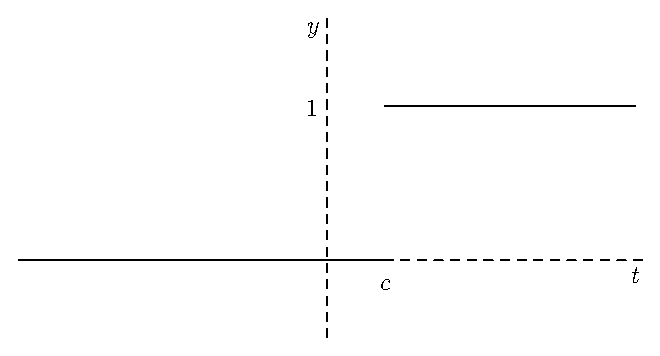
\includegraphics{201/step}
    \caption{Graph of the step function $u_c(t)$.}
    \label{step}
  \end{center}
\end{figure}

The Laplace transform of the step function is straightforward to calculate. If
we take $c>0$, then
\begin{align*}
\Laplace{}\(u_c(t)\) &=& \int_0^\infty u_c(t) e^{-st} dt
\\\nonumber
&=& \int_c^\infty e^{-st} dt
\\\nonumber
&=&\frac{e^{-cs}}{s}.
\end{align*}

The step function often shows up multiplied by other functions, as in the
following example.\\
\oexample{Solve the differential equation
\begin{align*}
y'=t u_c(t), \qquad y(0)=0
\end{align*}
using Laplace transforms.\\
}
{
Take the Laplace transform of both sides of the differential equation, yielding
\begin{align*}
sY &=& \Laplace{}\(t u_c(t)\) = \int_0^\infty t u_c(t) e^{-st} dt
= \int_c^\infty t e^{-st} dt
\\\nonumber
&=& \[t \frac{e^{-st}}{-s}\]_c^\infty - \int_c^\infty \frac{e^{-st}}{-s}dt
= \frac{-ce^{-sc}}{s} + \frac{e^{-sc}}{s^2}
\end{align*}
Thus,
\begin{align*}
Y = \frac{ce^{-sc}}{s} +\frac{e^{-sc}}{s^3}.
\end{align*}
From the table of  Laplace transforms, we know that
$\Laplace{}\(f(t-c)u_c(t)\)=e^{-cs}F(s)$, so
\begin{align*}
y = -c(t-c)u_c(t) + \frac{1}{2} (t-c)^2 u_c(t). \qed %FIXME: check
\end{align*}
}



\section{The Impulse Function}
While the step function describes functions which start suddenly (like turning
on a switch), the delta function, $\d(t)$, is slightly more complicated. It
describes processes that happen in an instant, like the impact from a hammer.
It is (loosely) defined as having the following properties:
\begin{align}
\boxed{
\delta(t) = \left\{ \begin{array}{ll}
         \infty & \mbox{if $t = 0$};\\
        0 & \mbox{if $t \neq 0$}.\end{array} \right.
}
\end{align}
and, for any function $f(t)$,
\begin{align}\label{deltaprop}
\boxed{\int_{-\infty}^\infty f(t) \delta(t)\, dt = f(0)}.
\end{align}
Approximations to the delta function are shown in figure~\ref{deltafig}.
\begin{figure}[htbp]
  \begin{center}
    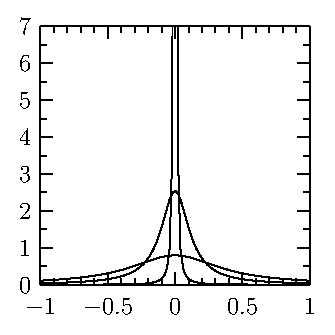
\includegraphics{201/delta}
    \caption{Approximations to $\d(x)$.}
    \label{deltafig}
  \end{center}
\end{figure}


\noindent\emph{Example}: Solve the following differential equation using
Laplace transforms.
\begin{align*}
2y'' + y' + 2y = \delta(t-5), \qquad y'(0)=y(0)=0
\end{align*}
\emph{Solution}: Taking the Laplace transform of both sides, we have
\begin{align}\label{exeq1}
\(2s^2 + s +2\) Y = e^{-5s}.
\end{align}
To see that the Laplace transform of $\delta(t-5)$ is $e^{-5s}$, consider the
definition of the Laplace transform:
\begin{align}
\mathcal{L}(\delta(t-5)) = \int_0^{\infty} e^{-st} \delta(t-5)\, dt.
\end{align}
If we let $\tau = t-5$, then this is the same as
\begin{align*}
\int_{-5}^{\infty} e^{-s(\tau+5)} \delta(\tau)\, d\tau .
\end{align*}
Then we apply equation (\ref{deltaprop}) to see that this is just $e^{-5s}$.

Going back to equation (\ref{exeq1}), solving for $Y$ and completing the
square yields
\begin{align*}
Y = \frac{e^{-5s}}{2} \( \frac{1}{\(s+\frac{1}{4}\)^2 + \frac{15}{16}} \).
\end{align*}
Finding the inverse transform is the hardest part of this process, but we can
break it up into smaller steps. We can just pull the $1/2$ out
because the Laplace transform is linear and then if we rearrange this, we get
\begin{align*}
Y = \frac{2}{\sqrt{15}}  \, e^{-5s}
\frac{\sqrt{\frac{15}{16}}}{\(s+\frac{1}{4}\)^2 + \frac{15}{16}}
= \frac{2}{\sqrt{15}}  \, e^{-5s} \,
\Laplace\[e^{\frac{-t}{4}}\sin\(\frac{\sqrt{15}}{4}t \) \]
\end{align*}
Now we have an exponential term, $e^{-5s}$, times a term that is the Laplace
transform of $e^{\alpha t}\sin(\beta t)$ with $\alpha=1/4$ and
$\beta=\sqrt{{15}/{16}}$. So we will use the Laplace
transform table to see that $Y$ is the Laplace transform of
\begin{align*}
y=\frac{2}{\sqrt{15}}u_5(t) e^{\frac{-(t-5)}{4}}\sin\(\frac{\sqrt{15}}{4}(t-5)\).
\qed
\end{align*}

\section{Problems}
\begin{enumerate}
\item Solve the integro-differential equation
  \begin{align*}
  y(t) + \int_0^t y(v) (t-v) dv = 1.
  \end{align*}
  \hidesolution{
    \begin{align*}
    \int_0^t y(v) (t-v) dv = \int_0^t (t-v) y(v) dv = t \ast y(t)
    \end{align*}
    so this equation is
    \begin{align*}
    y(t) + t \ast y(t) = 1.
    \end{align*}
    Recall that
    \begin{align*}
    \Laplace \{f \ast g\} = \Laplace \{f\} \Laplace \{g\}
    \end{align*}
    so the Laplace transform of this equation is
    \begin{align*}
    \Laplace \{y(t)\} + \Laplace \{ t \ast y(t) \} &=& \Laplace \{1 \} \\
    \Laplace \{y(t)\} + \Laplace \{t\} \Laplace \{y(t)\} &=& \Laplace \{1\} \\
    Y(s) + \frac{1}{s^2} Y(s) &=& \frac{1}{s} \\
    \left( 1 + \frac{1}{s^2} \right) Y(s) &=& \frac{1}{s} \\
    \frac{s^2 + 1}{s^2} Y(s) &=& \frac{1}{s} \\
    Y(s) &=& \frac{s^2}{s(s^2+1)} \\
    Y(s) &=& \frac{s}{s^2+1}.
    \end{align*}
    Then taking the inverse transform yields
    \begin{align*}
    y(t) = \Laplace^{-1} \( \frac{s}{s^2+1} \) = \cos t.
    \end{align*}
  }

  \item
    Find the Laplace transform of
    \begin{align*}
    f =
    \left\{ \begin{array}{ll}
      e^t & \mbox{if $t < c$};\\
      t^2 & \mbox{if $t \geq c$}.
    \end{array} \right.
    \end{align*}
    \hidesolution{
      \begin{align*}
      \mathcal{L}(f)
      &=& \int_0^c e^t e^{-st} \, dt + \int_c^\infty t^2 e^{-st} \, dt
      \end{align*}
      The first integral is
      \begin{align*}
      \int_0^c e^t e^{-st} \, dt = \left.\frac{e^{(1-s)t}}{1-s}\right|_0^c
      =\frac{e^{(1-s)c}-1}{1-s}.
      \end{align*}
      The second integral requires two integrations-by-parts:
      \begin{align*}
      \int_c^\infty t^2 e^{-st} \, dt
      &=& \left. t^2 \frac{e^{-st}}{-s}\right|_c^\infty
      -2 \int_c^\infty t \frac{e^{-st}}{-s} \, dt
      \\
      &=&\frac{c^2}{s} +\frac{2}{s}
      \[
      t \left.\frac{e^{-st}}{-s}\right|_c^\infty
      - \int_c^\infty \frac{e^{-st}}{-s}\,dt
      \]
      \\
      &=&\frac{c^2}{s} + \frac{2c}{s^2} + \frac{2}{s^3}.
      \end{align*}
      The Laplace transform of $f$ is then the sum, i.e.,
      \begin{align*}
      \mathcal{L}(f) =
      \frac{e^{(1-s)c}-1}{1-s}
      + \frac{c^2}{s} + \frac{2c}{s^2} + \frac{2}{s^3}.
      \end{align*}
    }

\item
  Prove that $\Laplace(f*g)=F(s)G(s)$.
  \hidesolution{TODO: write solution.}

\item
  Solve $y'' = t u_c(t)$, $y(0)=y'(0)=0$, for $y(t)$ using Laplace transforms.
  \hidesolution{
    Note that $tu_c(t) = (t-c)u_c(t) +cu_c(t)$. Then,
    \begin{align*}
    s^2 Y = \frac{e^{-cs}}{s^2} + \frac{e^{-cs}}{s},
    \implies Y =  \frac{e^{-cs}}{s^4} + \frac{e^{-cs}}{s^3}
    \end{align*}
    so
    \begin{align*}
    y = u_c(t) \(\frac{t^3}{3!} + \frac{t^2}{2!}\).
    \end{align*}
  }

\item
  Solve the IVP
  \begin{align*}
  y'' + y = M\d(t-1), \qquad y'(0)=y(0)=0.
  \end{align*}
  \hidesolution{
  TODO: write solution.
  }

\end{enumerate}



\chapter{Solving Systems of Differential Equations}

Up to now, we could have solved every problem with the method of variation
of parameters. You've probably noticed that some questions are easier to
solve with certain techniques than with others, of course, but VoP will handle
any nonhomogeneous part, so long as you can calculate the integral. Here's
something that it won't handle:
\\

\noindent\emph{Example}:
Solve the system of initial value problems for both $x$ and $y$:
\begin{align*}
x' &=& -y \qquad x(0)=0 \\
y' &=& \phantom{-}x \qquad y(0)=1 \\
\end{align*}
Well, you can actually solve this by doing tricky things like taking the
derivative of one of the equations, but let's use Laplace transforms:
\\

\noindent\emph{Solution}: The Laplace transform of the original system is
\begin{align*}
sX &=& -Y \\
sY-1 &=&\phantom{-}X.
\end{align*}
Solving for $Y$ yields
\begin{align}
\label{syseg1}
sY -1 = \frac{-Y}{s} \quad \implies \quad Y = \frac{s}{s^2+1}.
\end{align}
Taking the inverse Laplace transform of equation (\ref{syseg1}) gives us
\begin{align*}
y(t) = \cos t.
\end{align*}
We can solve for $X$ in a similar way, or just notice that $x=y'$, i.e.\
\begin{align*}
x(t) = -\sin t
\end{align*}

Systems of differential equations model situations where there are two or
more quantities being evolved, such as heat and reaction rate, or predator and
prey populations. While they are obviously of great use, they can get
quite complicated as the number of variables increases (and are greatly
simplified by writing them in terms of matrices).\\


\noindent\emph{Example}: Solve the following system of differential equations:
\begin{align*}
x' - 3x + 2y = \sin t\\
4x -y' - y = \cos t
\end{align*}
with initial conditions $x(0)=y(0)=0$.
\\

\noindent\emph{Solution}:\\
We take the Laplace transform of each equation and put in the initial
conditions, which yields
\begin{align*}
sX - 3X +2Y = \frac{1}{s^2+1}\\
4X -sY -Y = \frac{s}{s^2+1}.
\end{align*}
We can solve the second equation for X:
\begin{align*}
X = \frac{1}{4}\(\frac{s}{s^2+1} + (s+1)Y\)
\end{align*}
Put this into the first equation, so
\begin{align*}
\(s-3\)\(\frac{1}{4} \frac{s}{s^2+1} + \frac{s+1}{4}Y\) +2Y
= \frac{1}{s^2+1}
\end{align*}
which gives
\begin{align}
\label{sysY}
Y &=& -\frac{(s-4)(s+1)}{(s^2+1)(s^2-2s+5)} \\ \nonumber
&=& \frac{11s +7}{10(s^2+1)} + \frac{-11s + 5}{10(s^2-2s+5)}  \\ \nonumber
&=& \frac{11s}{10(s^2+1)} + \frac{7}{10(s^2+1)} +
\frac{-11}{10}\frac{s-1}{(s-1)^2 + 2^2}
-  \frac{3}{10}\frac2{(s-1)^2 + 2^2}
\end{align}
by partial fractions and completing the square in the last two terms. We are
now in a position to use an inverse Laplace transform to get $y(t)$:
\begin{align*}
y(t) = \frac{7}{10} \sin t + \frac{11}{10} \cos t
- \frac{11}{10}e^{t}\cos 2t - \frac{3}{10}e^{t}\sin 2t
\end{align*}
It now remains to solve for $x(t)$. We use the solution for $X$
and the Laplace transform of $y$. This is to say
\begin{align}
\label{sysX}
X &=& \frac{1}{4}\(\frac{s}{s^2+1} + (s+1)Y\)\\ \nonumber
 &=& \frac{-1 + 7s}{10(s^2+1)} + \frac{-7s + 15}{10(s^2-2s+5)} \\ \nonumber
 &=& \frac{7s}{10(s^2+1)} + \frac{-1}{10(s^2+1)} + \frac{-7}{10}
\frac{s-1} {(s-1)^2 + 2^2} +  \frac{2}{5}\frac{2}{(s-1)^2 + 2^2}
\end{align}
So we can now use an inverse Laplace transform to get $x(t)$.
\begin{align*}
x(t) = \frac{-1}{10} \sin t + \frac{7}{10} \cos t - \frac{7}{10}e^{t}\cos 2t
+ \frac{2}{5}e^{t}\sin 2t
\end{align*}

Alternatively, we could have solved this as a linear system, since
\begin{align*}
\[ \begin{array}{ll}
    (s-3) & 2\\
    4 & -(s+1)
  \end{array} \]
\( \begin{array}{l}
    X\\
    Y
  \end{array} \)
=
\( \begin{array}{l}
    \frac{1}{s^2+1}\\
    \frac{s}{s^2+1}
  \end{array} \)
\end{align*}
which is easily solved for $X$ and $Y$ to give
\begin{align*}
\( \begin{array}{l}
    X\\
    Y
  \end{array} \)
=
\frac{1}{s^2+1} \cdot \frac{1}{s^2-2s+5}
\( \begin{array}{l}
    3s+1\\
    s^2 -3s -4
  \end{array} \),
\end{align*}
which brings us to equations (\ref{sysY}) and (\ref{sysX}) with a lot less
work. \qed

\section{Problems}

\begin{enumerate}
  \item Solve the following system of differential equations:
    \begin{align*}
    \begin{array}{ll}
      x'=z, & \qquad x(0)=0\\
      y'=x, &\qquad y(0)=0 \\
      z'=y, &\qquad z(0)=1.
    \end{array}
    \end{align*}
    \hidesolution{
      Note: For the quiz, computing just $z(t)$ should be sufficient, since this
      takes students about 40 minutes.\\

      The Laplace transform gives us
      \begin{align*}
      sX &=& Z \\
      sY &=& X \\
      sZ-1 &=& Y
      \end{align*}
      Solving for $Z$, we have
      \begin{align*}
      Z &=& \frac{s^2}{s^3-1}
      = \frac{1}{3}\frac{1}{s-1}
      + \frac{1}{3} \frac{2s+1}{s^2 + s+ 1}\\
      &=& \frac{1}{3}\frac{1}{s-1}
      + \frac{1}{3} \frac{2s+1}{(s+\half)^2+ \frac{3}{4}}
      = \frac{1}{3}\frac{1}{s-1}
      + \frac{2}{3} \frac{s+\half}{(s+\half)^2+ \frac{3}{4}}
      \end{align*}
      which has inverse Laplace transformation
      \begin{align*}
      z = \frac{1}{3}e^t
      + \frac{2}{3}e^{-\frac{t}{2}} \cos \frac{\sqrt{3}}{2} t.
      \end{align*}
      Similarly, $sX=Z$ implies that
      \begin{align*}
      X = \frac{s}{s^3 -1}
      = \frac{1}{3}\frac{1}{s-1} - \frac{1}{3}\frac{s-1}{s^2+s+1}
      = \frac{1}{3}\frac{1}{s-1}
      - \frac{1}{3}\frac{s+\half}{(s+\half)^2+\frac{3}{4}}
      - \frac{1}{3}\frac{-3}{2}\frac{2}{\sqrt{3}}
      \frac{\sqrt{3}/2}{(s+\half)^2+\frac{3}{4}}
      \end{align*}
      so
      \begin{align*}
      x = \frac{e^t}{3}
      -e^{\frac{-t}{2}}\(
      \frac{1}{3}\cos \frac{\sqrt{3}}{2}t
      +\frac{1}{\sqrt{3}}\sin \frac{\sqrt{3}}{2}t
      \),
      \end{align*}
      and $sY=X$ implies that
      \begin{align*}
      Y = \frac{1}{s^3-1}
      = \frac{1}{3}\frac{1}{s-1} - \frac{1}{3}\frac{s+2}{s^2+s+1}
      = \frac{1}{3}\frac{1}{s-1}
      - \frac{1}{3}\frac{s+\half}{(s+\half)^2+\frac{3}{4}}
      - \frac{1}{3}\frac{3}{2}\frac{2}{\sqrt{3}}
      \frac{\sqrt{3}/2}{(s+\half)^2+\frac{3}{4}}
      \end{align*}
      so
      \begin{align*}
      Y = \frac{e^t}{3}
      +e^{\frac{-t}{2}}\(
      \frac{1}{3}\cos \frac{\sqrt{3}}{2}t
      -\frac{1}{\sqrt{3}}\sin \frac{\sqrt{3}}{2}t
      \).\qed
      \end{align*}
    }

  \item
    Solve the following system of differential equations
    \begin{align*}
    x' -y = e^t, \qquad x(0)=1.
    \\
    y' + x = e^t, \qquad y(0)=0.
    \end{align*}
    \hidesolution{
      The transform gives us
      \begin{align*}
      sX -1 -Y = \frac{1}{s-1}
      \\
      sY + X = \frac{1}{s-1}
      \end{align*}
      so
      \begin{align*}
      s^2 Y  + Y = \frac{-1}{s-1} -1 + \frac{s}{s-1}
      =- \frac{1}{s-1} -1 + \frac{s-1}{s-1} - \frac{1}{s-1}
      = \frac{-2}{s-1}.
      \end{align*}
      Thus,
      \begin{align*}
      Y = \frac{-2}{3} \(-\frac{s+1}{s^2+1} + \frac{1}{s-1} \)
      \end{align*}
      so
      \begin{align*}
      y = \frac{2}{3}\sin t + \frac{2}{3}\cos t - \frac{2}{3}e^t
      \text{ and } x = e^t-y'
      = -\frac{2}{3}\cos t + \frac{2}{3} \sin t + \frac{5}{3}e^t
      .\qed
      \end{align*}

    }

    \item
      Solve the system of differential equations
      \begin{align*}
      x'+y=0,\qquad x(0)=1
      \\
      y' = 2 \cosh(2t),\qquad y(0)=1
      \end{align*}
      \hidesolution{
      The second DE has transform
      \begin{align*}
      sY -1 = 6 \frac{s}{s^2-4} \implies Y =  6 \frac{1}{s^2-4} + \frac{1}{s}
      \end{align*}
      so
      \begin{align*}
      y = \sinh(t) +1
      \end{align*}
      and
      \begin{align*}
      x = \int \sinh(t) +1 dt = \cosh t +t +C
      \end{align*}
      with $C=0$ matching the initial condition. \qed
      }

\end{enumerate}


\chapter{Series Solutions to DEs}

A smooth function $f(t)$ can be approximated near a point $t=a$ by looking
at its derivatives. In fact, if $f$ is smooth enough, its value at any
given $t$ can be entirely determined by its behaviour at $t=a$.

The most basic approximation that we can make is that the function stays
constant. For example, a good guess for the temperature in ten minutes would
be what the temperature is now. That is, we approximate $f$ as
\begin{align*}
f(t) \approx f_0(t) = f(a).
\end{align*}
Now, it may be that the sun is shining, so we expect it to heat up. Then our
next approximation is to account for this using $f'(a)$, i.e.\
\begin{align*}
f(t) \approx f_1(t) = f(a) + f'(a) (t-a).
\end{align*}
As the sun sets, the rate of heating changes, so we need to add a term with
$f''(a)$, which gives us
\begin{align*}
f(t) \approx f_2(t) = f(a) + f'(a) (t-a) + \frac{f''(a)}{2}\(t-a\)^2,
\end{align*}
and so on. This is called a \emph{Taylor Polynomial Approximation} (or simply a
Taylor polynomial). It's easy to deal with both analytically and numerically,
and it can be used to get at least a basic understanding of just about any IVP.

The $n$th degree Taylor polynomial is
\begin{align}
\boxed{f_n(t) = f(a) + f'(a)(t-a) + \dots + \frac{f^{(n)}(a)}{n!} (t-a)^n
= \sum_{i=0}^n \frac{f^{(i)}(a)}{i!}(t-a)^i},
\end{align}
and it exists for any function $f$ whose first $n$ derivatives are smooth for
$t\in [a,t]$.
Let $R_n(t) = f(t) -f_n(t)$ denote the error associated with the $n$th Taylor
polynomial. Then, Taylor's theorem states that there exists a number
$\xi \in [a,t]$ where
\begin{align}
\boxed{R_n(t) = \frac{f^{(n+1)}(\xi)}{(n+1)!}(t-a)^{n+1}}.
\end{align}
So long as $\lim_{n\rightarrow \infty} R_n(t) =0$, $f_n$ will be a better and
better approximation as $n$ increases.


The Taylor series of $f$ is the limit of $f_n$ as $n\rightarrow\infty$, which is
\begin{align}
\boxed{\sum_{i=0}^\infty \frac{f^{(i)}(a)}{i!}(t-a)^i}.
\end{align}
The Taylor series for $f$ exists as long as every derivative of $f$ is
continuous (i.e.\ $f$ is \emph{analytic}), and is equal to $f$ if their
difference is zero (i.e.\ $\lim_{n\rightarrow \infty} R_n(t) =0$). Since these
things are equal, we can use this to solve equations. Of course, we need to
make sure that these series converge in order for our solution to make sense.
What's more, if $f$ is analytic, then the derivative of the sum is the sum
of the derivatives, which can greatly simplify things.\\

\oexample{
  Find the Taylor series for $f=e^x$ about $x=0$ and its interval of
  convergence.
}{
  First, we need to find the derivatives of $e^x$. This is easy, since
  \begin{align*}
  f^{(n)}(x) = \frac{d^n}{dx^n}e^x = e^x.
  \end{align*}
  Thus, $f^{(n)}(0)=e^0=1$, so the Taylor series is given by
  \begin{align*}
  \sum_{n=0}^\infty \frac{1}{n!} x^n.
  \end{align*}
  For what values of $x$ will this series converge? To determine this, we'll
  have to use a convergence test. Letting $A=\sum_{n=0}^\infty a_n$
  $B=\sum_{n=0}^\infty b_n$ be two series, our test are:
  \begin{enumerate}
  \item The comparison test: if
    $\lim_{n \rightarrow \infty} \abs{a_n/b_n} \in (0,\infty)$, then $A$
    converges if and only if $B$ converges.
  \item The ratio test: if
    $\lim_{n\rightarrow\infty}\abs{\frac{a_{n+1}}{a_n}}=c < 1$, then $A$
    converges.
  \item The root test: if $\lim_{n\rightarrow\infty}\abs{a_n}^{1/n}=c < 1$,
    then $A$ converges.
  \item The integral test: if there is a function $f$ with $f(n)=a_n$, then
    $A$ converges if and only if $\int_0^\infty f(t) dt$ is finite.
  \item The alternating series test: if $a_n = (-1)^n c_n$, then $A$
    converges so long as $\lim_{n\rightarrow\infty}c_n=0$ and each $c_n$ is
    smaller than $c_{n-1}$.
  \end{enumerate}
  Let's try the ratio test. That is, fix $x$ and look at
  \begin{align*}
  \lim_{n\rightarrow\infty} \frac{a_{n+1}}{a_n}
  = \lim_{n\rightarrow\infty}\frac{x^{n+1}/(n+1)!}{x^n/n!}
  =\lim_{n\rightarrow\infty}\frac{x}{n+1} =0 < 1.
  \end{align*}
  That is, for any $x\in \mathbb{R}$, $n+1$ will eventually be greater than
  $x$.  Thus, the limit is zero, and the series converges for all
  $x \in (-\infty,\infty) =\mathbb{R}$. \qed
}

In the above example, the series converged everywhere. This isn't always
the case: often, a series solution to a differential equation is only
valid in some neighbourhood of the initial conditions, and the series
becomes divergent when $\abs{t-a} > r$, and we call $r$ the radius of
convergence.\\

\oexample{
  Find the radius of convergence for the Taylor series for $f=\arctan(x)$
  about $x=0$.\\
}
{
  The Taylor series for $\arctan(z)$ is
  \begin{align*}
  \sum_{n=0}^\infty \frac{(-1)^n z^{2n+1}}{2n+1}
  \end{align*}
  Using the ratio test again, we look at
  \begin{align*}
  \abs{\frac{a_{n+1}}{a_n}} = \frac{z^{2(n+1)+1}/(2(n+1)+1)}{z^{2n+1}/(2n+1)}
  = \frac{z^2}{(2n+3)/(2n+1)}\rightarrow z^2
  \end{align*}
  Clearly, this limit is only less than one if $\abs{z}<1$. We still need to
  check the case when $\abs{z}=1$. This is pretty easy to do, since if $z=1$,
  the series is just
  \begin{align*}
  \sum_{n=0}^\infty \frac{(-1)^n}{2n+1},
  \end{align*}
  which converges by the alternating series test. Similarly, the series
  converges if $z=-1$. Thus, the interval of convergence is $\[-1,1\]$.
  \qed
}

Now that we can calculate Taylor series and know when they are valid, we
can use them to calculate solutions to differential equations. To simplify
matters, we will restrict ourselves to initial value problems
which begin at $t=0$, so that $a=0$ in all the above formulae. Now, we can
express the solution $y(t)$ as a Taylor series,
\begin{align*}
y = \sum_{n=0}^\infty a_n t^n .
\end{align*}
We assume that this solution is analytic, so we can take the derivative of the
series term-by-term. That is,
\begin{align*}
\dd{y}{t} = \dd{}{t}\sum_{n=0}^\infty a_n t^n
= \sum_{n=0}^\infty \dd{(a_n t^n)}{t} = \sum_{n=0}^\infty a_n n t^{n-1}
= \sum_{n=1}^\infty a_n n t^{n-1}
\end{align*}
(the last equality is because when $n=0$ we have that $a_n n t^{n-1}=0$, so we
can ignore the term with $n=0$). Since we know that $a_0=y(0)$, and $y(0)$ is
given by the initial conditions, we can solve for the rest of the $a_n$
recursively.\\
\oexample{Determine the solution to the IVP
\begin{align*}
y'(t) = t^2 +t, \qquad y(0)=1
\end{align*}
using a Taylor series for $y$.\\
}
{
  Let
  \begin{align*}
  y =\sum_{n=0}^\infty a_n t^n.
  \end{align*}
  Then, $a_0=y(0)=1$, and
  \begin{align*}
  y'(t) = \sum_{n=1}^\infty a_n n  t^{n-1} = t^2 +t.
  \end{align*}
  Matching like powers of $t$, we have
  \begin{align*}
  2 a_2 t = t, \qquad 3 a_3 t^2 = t^2
  \end{align*}
  and $a_n n t^n =0$ for $n=1$ and all $n \geq 4$. Thus, $a_1 =0$, $a_2=\half$,
  and $a_3 = \frac{1}{3}$. The solution is then
  \begin{align*}
  y(t) = 1 +\frac{t^2}{2} +\frac{t^3}{3}.
  \end{align*}
}
It was easy to isolate all of the $a_n$'s in the previous example, since $y'$
appeared alone in the IVP. It's usually necessary to solve for $a_n$
recursively.\\
\oexample{
  Solve the IVP
  \begin{align*}
  y'' = -y, \qquad y(0) =1, \qquad y'(0)=0.
  \end{align*}
  using a Taylor series for $y$.\\
}
{
  Again, let $y=\sum_{n=0}^\infty a_n t^n$. Then
  \begin{align*}
  y'' = \sum_{n=2}^\infty a_n n (n-1)t^{n-2}.
  \end{align*}
  The differential equation is then
  \begin{align}
  \label{serieseg}
  \sum_{n=2}^\infty a_n n (n-1)t^{n-2} = -\sum_{n=0}^\infty a_n t^n
  \end{align}
  If we set $m=n-2$, then we can shift the summation index on the LHS to start
  at zero. That is,
  \begin{align*}
  y'' = \sum_{n=2}^\infty a_n n (n-1)t^{n-2}
  = \sum_{m=0}^\infty a_{m+2}(m+2)(m+1)t^m.
  \end{align*}
  This makes it much easier to solve \eqref{serieseg}, since we now have
  \begin{align*}
  \sum_{m=0}^\infty a_{m+2}(m+2)(m+1)t^m =  -\sum_{n=0}^\infty a_n t^n
%  \end{align*}
%  \begin{align*}
  \implies \sum_{n=0}^\infty \[a_{n+2}(n+2)(n+1) +a_n \]t^n =0
  \end{align*}
  In order for this to hold for all $t$ in a neighbourhood of $t=0$, it must
  be that
  \begin{align}
  \label{seriesrec}
  a_{n+2}(n+2)(n+1) +a_n =0.
  \end{align}
  From the initial conditions, we have $a_0=1$ and $a_1=0$. We can solve
  for $a_2$ by setting $n=0$ in equation \eqref{seriesrec}, which yields
  \begin{align*}
  a_2 \times 2 \times 1 = -1, \implies a_2=-\half.
  \end{align*}
  If we have $n$ even, then $n=2p$, and
  \begin{align*}
  a_{2p} = -\frac{a_{2p-2}}{2p(2p-1)} = \frac{a_{2p-4}}{2p(2p-1)(2p-3)(2p-4)}
  = \dots
  = \frac{(-1)^p a_0}{(2p)!} =\frac{(-1)^p}{(2p)!}
  \end{align*}
  It's easy to see that $a_3=0$, and, in fact, $a_n=0$ if $n$ is odd. Since
  we now know the values for all the $a_n$, we can write the solution:
  \begin{align*}
  y(t) = \sum_{n=0}^\infty t^n
  \left\{\begin{array}{ll}
    \frac{(-1)^{n/2}}{n!} & \mbox{if $n$ is even};\\
    0 & \mbox{if $n$ is odd}.
  \end{array} \right.
  = \sum_{p=0}^\infty \frac{(-1)^p t^{2p}}{(2p)!}. \qed
 \end{align*}
 You may recall from previous classes that this is just the Taylor series
 for $\cos t$.
}




\section{Problems}
\begin{enumerate}
\item Determine the convergence set of the series
  \begin{align*}
  \sum_{n=0}^\infty \frac{3^n}{n} (x-2)^n.
  \end{align*}
  \hidesolution{
    For this series $a_n = \frac{3^n}{n}$ and $x_0 = 2$, so
    \begin{align*}
    L = \lim_{n \to \infty} \left| \frac{a_{n+1}}{a_n} \right|
    = \lim_{n \to \infty} \left| \frac{3^{n+1}}{n+1} / \frac{3^n}{n} \right|
    = \lim_{n \to \infty}
    \left| \frac{3 \cdot 3^n}{n+1} \times \frac{n}{3^n} \right|
    = \lim_{n \to \infty} \left| 3 \frac{n}{n+1} \right|
    = 3 \lim_{n \to \infty} \frac{n}{n+1}
    = 3
    \end{align*}
    and then
    \begin{align*}
    \rho = \frac{1}{L} = \frac{1}{3}.
    \end{align*}
    So the series converges (absolutely) on
    \begin{align*}
    (x_0 - \rho, x_0 + \rho) = \left( 2 - \frac{1}{3}, 2 + \frac{1}{3} \right)
    = \left( \frac{5}{3}, \frac{7}{3} \right).
    \end{align*}
    It remains to check if the series converges at the endpoints of this
    interval.  At $x = \frac{5}{3}$, we have
    \begin{align*}
    \sum_{n=0}^\infty \frac{3^n}{n} \left( \frac{5}{3} - 2 \right)^n
    = \sum_{n=0}^\infty \frac{3^n}{n} \left( \frac{-1}{3} \right)^n
    = \sum_{n=0}^\infty \frac{3^n}{n} \times \frac{(-1)^n}{3^n}
    = \sum_{n=0}^\infty \frac{(-1)^n}{n}
    \end{align*}
    which is the alternating harmonic series which converges (recall that an
    alternating series converges $\iff$ the terms go to 0),
    and at $x = \frac{7}{3}$ we have
    \begin{align*}
    \sum_{n=0}^\infty \frac{3^n}{n} \left( \frac{7}{3} - 2 \right)^n
    = \sum_{n=0}^\infty \frac{3^n}{n} \left( \frac{1}{3} \right)^n
    = \sum_{n=0}^\infty \frac{1}{n}
    \end{align*}
    which is the harmonic series which diverges. So the convergence set is
    \begin{align*}
    \left[ \frac{5}{3}, \frac{7}{3} \right).
    \end{align*}
  }

  \item
    Determine the first four non-zero terms of the Taylor series of the
    solution to the Chebyshev equation,
    \begin{align*}
    (1-x^2)y'' - xy' +p^2 y=0
    \end{align*}
    with initial conditions $y(0)=a_0$, $y'(0)=a_1$.
    \hidesolution{
      TODO: write the solution
    }

  \item
    Determine the fourth degree Taylor polynomial for the solution to
    \begin{align*}
    (y')^2 + y = e^x, \qquad y(0)=0.
    \end{align*}
    \hidesolution{
      The first four terms of $y'$ are $a_1 + 2 a_2 x +3 a_3 x^2 + 4 a_4 x^3$.
      The first four terms of $y'^2$ are therefore
      \begin{align*}
      (y') + y \approx a_0+a_1^2 + x\(a_1 +4 a_1 a_2 \)
      + x^2 \(a_2+ 4a_2^2+6 a_1 a_3 \)
      +x^3\(a_3 + 8a_1 a_4 +12 a_2 a_3 \)
      \end{align*}
      and equal
      \begin{align*}
      e^x \approx 1 + x + \frac{x^2}{2} + \frac{x^3}{6}
      \end{align*}
      Matching order-by-order, we have
      \begin{align*}
      \begin{array}{ll}
	\O(1): & a_0 + a_1^2 =1 \\
	\O(x): & a_1(1+ 4 a_2) =1\\
	\O(x^2): & a_2 + 4a_2^2 + 6 a_1a_3 =\half \\
	\O(x^3): & a_3 + 8 a_1 a_4 + 12 a_2a_3=\frac{1}{6} \\
      \end{array}
      \end{align*}
      Subbing back into these equations, we get
      \begin{align*}
      a_1=1, \qquad a_2 =0, \qquad a_3=\frac{1}{12}, \qquad a_4=\frac{1}{96},
      \end{align*}
      and
      \begin{align*}
      y(x) \approx x + \frac{x^3}{12} + \frac{x^4}{96}.
      \end{align*}
    }

  \item
    Solve
    \begin{align*}
    y' = \frac{1}{1+x^2}, \qquad y(0)=0
    \end{align*}
    using a Taylor series. Do not leave your solution as an infinite series,
    but equate it to a known function.
    \hidesolution{
      This is just $y(x)=\arctan x$.
    }

%too complicated--needs help
% \item
%    The pendulum is often approximated as a harmonic oscillator. The full
%    system is nonlinear in $y$, since
%    \begin{align}
%    y''=-\sin y,
%    \end{align}
%    which reduces to the usual case, $y''=-y$, for small $y$. A slightly
%    better approximation would be to approximate $\sin$ to higher order, as in
%    \begin{align}
%    \label{pend3}
%    y''=-y + \frac{y^3}{3!}.
%    \end{align}
%    Provide a third-order Taylor polynomial approximation to the solution of
%    \eqref{pend3}.
%
%    If we take \eqref{pend3} and multiply it by $y'$, we can get the energy
%    equation for the system, namely
%    \begin{align}
%    y' y'' = \ddt{y'^2/2}
%    = \ddt{}\int^{y(t)}\(-\hat{y} + \frac{\hat{y}^3}{3!}\) d\hat{y}.
%    \end{align}
%    Thus, the energy of the system, $E=\frac{y'^2}{2}
%    + \int^{y(t)}\(\hat{y} - \frac{\hat{y}^3}{3!}\) d\hat{y}$, is conserved,
%    since
%    \begin{align}
%    \ddt{}\(\frac{y'^2}{2}
%    + \int^{y(t)}\(\hat{y} - \frac{\hat{y}^3}{3!}\) d\hat{y}\) =0.
%    \end{align}
%    Based on the conservation of energy, what do you expect to happen at large
%    $y$? Why might $y''=-y$ be a better approximation at large $y$ than
%    $y''=-y + {y^3}/{3!}$ is?
%    \hidesolution{
%      TODO: work out the approximation
%
%      The reason that the third-order approximation breaks down is that
%      the energy goes to $-\infty$ for large $\abs{y}$, so the solution will
%      grow unboundedly.
%    }

  \item
    Give a recursion formula for $a_n$ if
    \begin{align*}
    a_{3n+1} = \frac{a_1}{(3n+1)\times (3n) \times (3n-2) \dots
      6 \times 4 \times \times 3}.
    \end{align*}

  \item
    Given the recursion relationship
    \begin{align*}
    a_n = \frac{-2}{n^2}a_{n-1},
    \end{align*}
    find $a_n$ explicitly.

  \item
    Given the recursion relationship
    \begin{align*}
    a_{n+4} = \frac{-k^2}{(n+4)(n+3)} a_{n-1},
    \end{align*}
    with $k$ a constant, find $a_n$ explicitly.

  \item Solve the differential equation
    \begin{align*}
    y'' - 2 x y' + \l y=0,
    \end{align*}
    with $\l$ a constant, using a Taylor series about $x=0$. For what values
    of $\l$ is the solution a polynomial?

\end{enumerate}



\chapter{Series Solutions to DEs at Regular Singular Points}
%Let $p(t), q(t)$ be analytic functions (ie, they admit power series
%representations).
Differential equations of the form
\begin{align}
\label{singode}
y'' + p(t)y' + q(t)y=0
\end{align}
can behave poorly at $t=0$, and may not admit solutions of the form
$y(t) =\sum_{n=0}^\infty a_n t^n$. However, we can still solve these problem
by modifying the series expansion. The easiest case is when the singular
point is a regular singular point, for which we use \emph{the method of
Froebenius}.

The point $t=0$ is a \emph{singular point} if either
$\lim_{t \rightarrow 0}p(t)=\infty$ or  $lim_{t \rightarrow 0}q(t)=\infty$.

The point $t=0$ is a \emph{regular singular point} of \eqref{singode} if
the two limits $\lim_{t\rightarrow 0} t p(t) =p_0$
and $\lim_{t\rightarrow 0} t^2 q(t) =q_0$
exist and are finite. Series solutions at regular singular points are of the
form
\begin{align}
\boxed{y(t) = \sum_{n=0}^\infty a_n t^{n+r}},
\end{align}
for some $r\in\mathbb{C}$ such that $a_0 \neq 0$.

Since we now have one more variable for which to solve (i.e.\ $r$ in addition
to $a_0, a_1,\dots$), we require one more equation in order to determine the
solution uniquely. Then if we take the first and second derivative of
$y(t) = \sum_{n=0}^\infty a_n t^{n+r}$ and put them into the left-hand side of
equation \eqref{singode}, we can see that the
leading-order (which is to say the $t^{r-2}$) coefficient is
\begin{align*}
a_0 r(r-1)t^{r-2} + a_0 \frac{p_0}{t} r t^{r-1} + a_0 \frac{q_0}{t^2} t^r
\end{align*}
In order to satisfy equation \eqref{singode}, this equation must equal $0$.
We can multiply by $t^2$ and since $a_0 \neq 0$, we see that
\begin{align}
\boxed{\implies r(r-1) + p_0 r  + q_0=0}.
\end{align}
This is called the \emph{indicial equation}. It's a quadratic so it has two
solutions, $r=r_1,r_2$.

If we have two distinct roots with $Re(r_1) > Re(r_2)$, we're fine, and we
have two linearly independent solutions
\begin{align}
\boxed{y_1(t) = \sum_{n=0}^\infty a_n t^{n+r_1}}
\quad\mbox{  and  }\quad
\boxed{y_2(t) = \sum_{n=0}^\infty b_n t^{n+r_2}}.
\end{align}
If $r_1=r_2$, then our solutions are
\begin{align}
\boxed{y_1(t) = \sum_{n=0}^\infty a_n t^{n+r_1}}
\quad\mbox{  and  }\quad
\boxed{y_2(t) = \ln(t) y_1(t) + \sum_{n=0}^\infty b_n t^{n+r_1}}.
\end{align}
If $r_1-r_2$ is an integer, then we have yet another possibility, i.e.\ that
\begin{align}
\boxed{y_1(t) = \sum_{n=0}^\infty a_n t^{n+r_1}}
\quad\mbox{  and  }\quad
\boxed{y_2(t) = C\ln(t) y_1(t) + \sum_{n=0}^\infty b_n t^{n+r_1}},
\end{align}
for some constant $C\in\mathbb{R}$.

Once one has determined $r_1$ and $r_2$, the constants $a_n$ and $b_n$ can
be determined by matching powers as per the previous section.

\oexample{
  Consider Bessel's equation,
  \begin{align}
  \label{bessel}
  t^2 y'' + ty' + (t^2-\alpha^2)y=0.
  \end{align}
}{
  We can divide Bessel's equation by $t^2$ to get it in the form of
  \eqref{singode}, that is
  \begin{align*}
  y''  + \frac{1}{t}y' + \(1-\frac{\alpha^2}{t^2}\)y=0,
  \end{align*}
  which is clearly singular. We can identify $p=1/t$, and
  $q=1-\frac{\alpha^2}{t^2}$. Then,
  \begin{align*}
  p_0 = \lim_{t\rightarrow 0} t p(t) =1, \quad \text{and}\quad
  q_0 = \lim_{t\rightarrow 0} t^2 q(t) =-\alpha^2.
  \end{align*}
  The indicial equation is then
  $r(r-1) +r -\alpha^2 =0 \implies r_{1,2} = \pm \alpha$.  Thus,
  \begin{align*}
  y_1\phantom{''} &=& \sum_{n=0}^\infty a_n t^{n+\alpha} \\
  y_1'\phantom{'}  &=& \sum_{n=0}^\infty a_n (n+\alpha)t^{n+\alpha-1}, \\
  y_1'' &=& \sum_{n=0}^\infty a_n (n+\alpha)(n+\alpha-1)t^{n+\alpha-2}.
  \end{align*}
  Putting this into \eqref{bessel}, we have
  \begin{align*}
  \sum_{n=0}^\infty a_n\[(n+\a)(n+\a-1) + (n+\a) - \a^2  \]t^{n+\alpha}
  + \sum_{n=0}^\infty a_n t^{n+2+\alpha}=0.
  \end{align*}
  Changing the index of the second sum, we have
  \begin{align*}
  \sum_{n=0}^\infty a_n\[(n+\a)(n+\a-1) + (n+\a) - \a^2  \]t^{n+\alpha}
  + \sum_{n=2}^\infty a_{n-2} t^{n+\alpha}=0.
  \end{align*}
  The $a_0$ and $a_1$ terms are determined by initial conditions. For
  $n\geq 2$, the terms must cancel, so we have
  \begin{align*}
  a_n\[\(n+\a\)^2 - \a^2\]t^{n+\alpha}  + a_{n-2} t^{n+\alpha}=0
  \end{align*}
  which implies that
  \begin{align*}
  a_n = \frac{-a_{n-2}}{\(n+\a\)^2 - \a^2} =  \frac{-a_{n-2}}{n(n+ 2\a)}.
  \end{align*}
  Associating $y_1$ with $a_0=1$ and $a_1=0$, we can set $n=2m$, so the
  recursion relationship is
  \begin{align}
  a_{2m} = \frac{-a_{2(m-1)}}{2m (2m+2\a)} = \frac{-a_{2(m-1)}}{2^2m (m+\a)}.
  \end{align}
  Solving the recursion relationship then yields
  \begin{align}
  a_{2m} = \frac{(-1)^ma_0}{2^{2m}m! (m+\a)(m+\a-1)\dots(1+\a)}.
  \end{align}
  The solution is then
  \begin{align}
  \label{bessel1}
  y_1 = \sum_{m=0}^\infty
  \frac{(-1)^m}{2^{2m}m! (m+\a)(m+\a-1)\dots(1+\a)(\a)} t^{m+\alpha}.  \qed
  \end{align}
We can simplify this a little by setting $a_0=1/(2^\a\G(\a+1))$. Then we would
get the standard form of Bessel's function of the first kind of order $\a$,
  \begin{align*}
  J_\alpha(t) = \sum_{n=0}^\infty \frac{(-1)^n}{n!\G(1-\a+n)}
  \(\frac{t}{2}\)^{2n-\a}.
  \end{align*}
Here $\G(x)$ is called the Gamma function and it is just an extension of the
factorial function. So in particular, when $\alpha=0$, we get
  \begin{align*}
  J_0(t) = \sum_{n=0}^\infty \frac{(-1)^n t^{2n}}{2^{2n}(n!)^2}.
  \end{align*}
% Too messy and complicated- fixed above
%  Now, we can simplify this slightly, by using the gamma function. The
%  Gamma function,
%  \be
%  \G(x) = \int_0^\infty t^{x-1} e^{-t} \, dt,
%  \end{align}
%  is a generalization of the factorial. The key step is that
%  \be
%  \G(x+1) = x \G(x),
%  \end{align}
%  which can be derived using integration by parts. If $x$ is an integer, this
%  gives us $\G(x+1)=x!$, since $\G(0)=1$. If we set $x=m+\a+1$, then
%  \begin{align}
%  \G(m+\a+1) &=& (m+\a) \G(m+\a) = (m+\a)(m+\a-1)\G(m+\a-1) = \dots \\\nonumber
%  &=& (m+\a)(m+\a-1) \dots (2+\a)(1+\a)\G(\a+1).
%  \end{align}
%  We can then write \eqref{bessel1} as
%  \begin{align}
%  y_1 = \sum_{m=0}^\infty
%  \frac{(-1)^m}{2^{2m}m! \G(m+\a+1)/\G(\a+1)} t^{m+\alpha}.
%  \end{align}
%
%  Setting $a_0=1/(2^\a\G(\a+1))$, we have the standard form of Bessel's
%  function
%  of the first kind of order $\a$,
%  \begin{align}
%  J_\alpha(t) = \sum_{n=0}^\infty \frac{(-1)^n}{n!\G(1-\a+n)}
%  \(\frac{t}{2}\)^{2n-\a}. \qed
%  \end{align}
}



\section{Problems}

\begin{enumerate}

  \item Find a general solution to the Cauchy-Euler (equidimensional) equation,
    \begin{align*}
    (\pi x)^2 y'' (x) + \pi(\pi-2)xy' (x) + y(x) = 0, \quad x > 0.
    \end{align*}
    \hidesolution{
      Rewrite this equation as
      \begin{align*}
      \pi^2 x^2 y'' (x) + (\pi^2 - 2\pi)xy' (x) + y(x) = 0.
      \end{align*}
      We substitute $y = x^r$ to find a solution. The indicial equation is
      \begin{align*}
      \pi^2 r^2 + (\pi^2 - 2\pi - \pi^2) r + 1 = \pi^2 r^2 - 2 \pi r + 1
      = (\pi r - 1)^2 = 0
      \end{align*}
      which has repeated root $r = \frac{1}{\pi}$.  So a general solution is
      \begin{align*}
      y(x) = C_1 x^\frac{1}{\pi} + C_2 x^\frac{1}{\pi} \ln x
      = C_1 \sqrt[\pi]{x} + C_2 \sqrt[\pi]{x} \ln x, \quad x > 0.
      \end{align*}
    }

  \item Find the solution to Bessel's equation corresponding to $r=-\a$,
    assuming that $2\a$ is not an integer.
    \hidesolution{
      TODO: add solution
    }

  \item Find the first solution (i.e.\ $y_1$ in the above notation) to the
    differential equation
    \begin{align*}
    x^2 y'' - xy' + (1-x)y=0
    \end{align*}
    \hidesolution{
      We have $p=-1/x$ and $q=(1-x)/x^2 = 1/x^2-1/x$. Then
      \begin{align*}
      p_0 = \lim_{x\rightarrow 0^+} x p(x)=-1, \qquad
      q_0 = \lim_{x\rightarrow 0^+} x^2 q(x)=1.
      \end{align*}
      The indicial equation is
      \begin{align*}
      r(r-1)-r+1=0 \implies r_1=r_2=1
      \end{align*}
      $y_1$ is given by
      \begin{align*}
      y = t^1 \sum_{n=0}^\infty a_n t^n,
      \end{align*}
      which gives
      \begin{align*}
      \sum_{n=1}a_n(n+1)(n)t^{n+1} - \sum_{n=1}a_n(n+1)t^{n+1}
      + \sum_{n=0}a_nt^{n+1} - \sum_{n=0}a_nt^{n+2}.
      \end{align*}
      The order $t$ term cancels out, leaving us free to determine $a_0$ by
      the initial conditions. We are then left with
      \begin{align*}
      \sum_{n=1}^\infty \[a_n(n+1)(n)-a_n(n+1)+a_n - a_{n-1}\]t^{n+1}=0,
      \implies a_n n^2 = a_{n-1}
      \end{align*}
      which yields
      \begin{align*}
      y_1 = a_0\sum_{n=0}^\infty \frac{t^{n+1}}{(n!)^2}.
      \end{align*}
    }

\end{enumerate}



\chapter{Partial Differential Equations}
Let $y(x,t)$ be the temperature of a one-dimensional rod with thermal
conductivity $k$. The equation that describes the evolution of $y$ is
called the heat equation:
\begin{align*}
\pp{y}{t} =  k\pptwo{y}{x}.
\end{align*}
This is an important example of a partial differential equation (PDE), in which
the derivatives with respect to one variable are related to derivatives with
respect to another variable, in this case $\partial/\partial t$ and
$\partial/\partial x$.

The basic technique for solving partial differential equations is to transform
it into an ordinary differential equation, which we can then solve using any
of the techniques that we have discussed so far. One very powerful technique
to do this is to transform the function $y$ into a \emph{Fourier series}.

\section{Separation of Variables}
As in the previous section, we use a series solution for $y$ and expand around
 $x=0$. However, instead of the coefficients being constant, we allow them to
be functions of time, and, instead of using $x^n$, we let $X_n(x)$ be a more
general function of $x$. That is, we let
\begin{align}
\boxed{y = \sum_{n=0}^\infty T_n(t) X_n(x)}.
\end{align}
As you will see in the next lab, we can choose the functions $X_n$ in a way
that makes the PDE solvable. For now, let's consider the case where the $X_n$
are either sine or cosine, i.e.\ when $y$ is a Fourier sine or cosine series.

\section{Fourier Cosine and Sine Series}
Consider functions that are periodic with period $2T$.
If we set $X_n =\cos(n \pi x/T)$, we have the \emph{Fourier cosine series} for
$f(x)$,
\begin{align*}
\frac{a_0}{2} + \sum_{n=1}^\infty a_n \cos\(\frac{n \pi x}{T}\)
\end{align*}
(note the annoying $1/2$ on the first term). Setting $X_n=\sin(n \pi x/T)$,
we get the \emph{Fourier sine series} for $f(x)$,
\begin{align*}
\sum_{n=1}^\infty b_n \sin\(\frac{n \pi x}{T}\)
\end{align*}
The coefficients $a_n$ and $b_n$ are determined by integration, with
\begin{align}\label{fouriercoeff}
\boxed{a_n = \frac{1}{T} \int_{-T}^T f(x) \cos\(\frac{n \pi x}{T}\) \, dx},
\quad \text{and} \quad
\boxed{b_n = \frac{1}{T} \int_{-T}^T f(x) \sin\(\frac{n \pi x}{T}\) \, dx}.
\end{align}
More generally, the \emph{Fourier series} for $f(x)$ is the sum of these, i.e.\
\begin{align*}
\boxed{\frac{a_0}{2} + \sum_{n=1}^\infty \[ a_n \cos\(\frac{n \pi x}{T}\)
+ b_n \sin\(\frac{n \pi x}{T}\) \]}.
\end{align*}
Often, we just look at functions that have period $2\pi$, which makes for the
simpler formulae,
\begin{align}\label{nicefourier}
&&\frac{a_0}{2} + \sum_{n=1}^\infty \[ a_n \cos\(nx\)
+ b_n \sin\(nx\) \] ;
\\ \nonumber
&&a_n = \frac{1}{\pi} \int_{-\pi}^\pi f(x) \cos\(n x\) \, dx,
\\ \nonumber
&&b_n = \frac{1}{\pi} \int_{-\pi}^\pi f(x) \sin\(n x\) \, dx,
\end{align}
which we will refer to as ``the'' Fourier series, unless otherwise stated.


Well, now we have yet another series that we can derive from a given function,
but we have to show that the series converges to the function if we
want to do anything useful. For this we have the following lemma:
\begin{theorem}[Riemann-Lebesque lemma]
If $\int_{-\infty}^\infty \abs{f(x)} dx$ exists, then
\begin{align}
\lim_{z\rightarrow \pm \infty}\int_{-\infty}^\infty f(x) e^{izx} dx =0
\end{align}
which implies that
\begin{align*}
\lim_{n\rightarrow \infty} a_n =0 \qquad \text{and} \qquad
\lim_{n\rightarrow \infty} b_n =0,
\end{align*}
and
\begin{align*}
f(x) = \frac{a_0}{2} + \sum_{n=1}^\infty \[ a_n \cos(nx) + b_n \sin(nx) \].
\end{align*}
%FIXME: should the limits of integration be $(-\pi,\pi)$ for the series (as
%opposed to the transform)? Also, uniqueness?
\end{theorem}

The Fourier series is the expression of a function as the sum an infinite series
of waves with different amplitudes. That is, we transform from ``$x$-space'' to
``frequency-space'', which can be incredibly useful. For example, the
\texttt{Ogg Vorbis} audio format is just a modified cosine-series. Fourier
series (and Fourier transforms, which are not covered in this course) lie at
the heart of signal analysis. In terms of solving PDEs, we make use of the
fact that
\begin{align*}
\ddtwo{}{x}\sin(nx) = -n^2 \sin(nx),
\end{align*}
(i.e.\ that sine is an Eigenfunction of $\ddtwo{}{x}$) to turn differential
equations into algebraic equations. But more on that later. First, let's just
find the Fourier series for a normal function.

\oexample{
Find the Fourier series of
\begin{align*}
f(x) = x
\end{align*}
}{
To find the Fourier series, we just need to determine $a_n$ and $b_n$ using
equation~\eqref{nicefourier}. The coefficients for the cosine series are
\begin{align*}
a_n &=& \frac{1}{\pi}\int_{-\pi}^\pi x \cos(nx)\, dx
\\\nonumber
&=& \frac{1}{\pi}\[ \left.x \frac{\sin(nx)}{n} \right|_{-\pi}^{\pi}
-\int_{-\pi}^\pi \frac{\sin(nx)}{n}\, dx \]
\\\nonumber
&=& \frac{1}{\pi}
\[0 - \frac{1}{n^2}\left. \cos(nx) \right|_{-\pi}^{\phantom{-}\pi} \] =0.
\end{align*}
This could have been expected, since $f(x)=x$ is an odd function, and $\cos(nx)$
is even, and the integration domain is symmetric. Notice, then, that the
cosine series of a function is equal to the even part of the function. Now,
for the sine series, we have
\begin{align*}
b_n &=& \frac{1}{\pi} \int_{-\pi}^\pi x \sin(nx)\, dx
\\\nonumber
&=& \frac{1}{\pi} \[ \left.\frac{-x\cos(nx)}{n}\right|_{-\pi}^\pi
                    - \int_{-\pi}^\pi \frac{-\cos(nx)}{n}\, dx  \]
\\\nonumber
&=& \frac{1}{\pi}\[\frac{-\pi\cos(\pi n)}{n} - \frac{-\pi\cos(-n\pi)}{n} -0 \]
\\\nonumber
&=& \frac{1}{\pi}\[\frac{-2\pi}{n}\cos(n \pi)\]
\\\nonumber
&=&\frac{-2 (-1)^n}{n} = (-1)^{n+1}\frac{2}{n}.
\end{align*}
The Fourier series for $f(x)=x$ is then
\begin{align}
\label{Fourierx}
x = 2 \sum_{n=1}^\infty  \frac{(-1)^{n+1}}{n} \sin(nx). \qed
\end{align}
This does indeed converge to $f(x)=x$ around $x=0$, as can be seen in
figure~\ref{fourierx}.
\begin{figure}[htbp]
  \begin{center}
    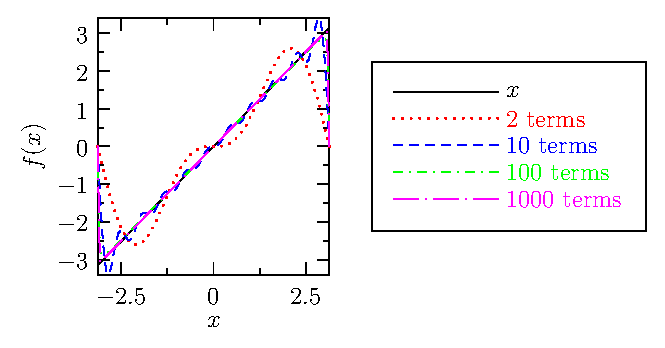
\includegraphics{201/fourierx}
    \caption{Fourier series approximations to $f(x)=x$.}
    \label{fourierx}
  \end{center}
\end{figure}
}

%TODO: something about orthogonality? More examples?

\section{Problems}

\begin{enumerate}
  \item
    What are the Fourier sine and cosine series for
    $y=\sin x$?
    \hidesolution{
      Students should make use of the orthogonality property for $\sin nx$ and
      $\sin mx$, $n \neq m$.
    }
  \item
    What is the Fourier series for $ f(x) = \d(x-1)$?

  \item What is the Fourier series in $x$ for $f(x,t)$ if
    \begin{align}
    f(x,t) =
    \left\{ \begin{array}{ll}
      -t           & \mbox{if $x < 0$};\\
      \phantom{-}t & \mbox{if $x \geq 0$}?
    \end{array} \right.
    \end{align}

\end{enumerate}


\chapter{Partial Differential Equations: Actually Solving Them}

Let us now return to the heat equation,
\begin{align}
\label{heateq}
\pp{y}{t} = \beta \frac{\partial^2y}{\partial x^2},
\end{align}
and add some \emph{initial conditions}
\begin{align*}
y(x,0)=f(x),
\end{align*}
and \emph{boundary conditions}
\begin{align}
\label{homdibc}
y(0,t)=0, \qquad y(\pi,t)=0.
\end{align}
Physically, this corresponds to modelling the temperature on a rod of length
$2\pi$ in contact at both ends with a heat sink with temperature $0$ (note
that this is not necessarily absolute zero: if we take $y=y+C$, the equation
remains the same, so our base temperature is arbitrary.) The
rod starts with the temperature at position $x$ given by $f(x)$.

We'll solve this using separation of variables:
\begin{align}\label{heatF}
y = \sum_{n=0}^\infty T_n(t) X_n(x),
\end{align}
where we have taken $X_n(x)$ to be orthogonal\footnote{That is, if $n\neq m$,
then $\int_0^\pi X_n(x) X_m(x) dx =0.$ This is the case with elements of
$\{\cos(nx),\sin(nx),n=0,1,\dots \}$.}.
Putting equation \eqref{heatF} into equation \eqref{heateq}, we get
\begin{align}\label{heats}
\sum_{n=0}^\infty \ddt{T_n(t)}X_n(x)
=\beta\sum_{n=0}^\infty T_n(t)\ddtwo{X_n(x)}{x}
\end{align}
Now, since the $X_n$'s are orthogonal, this actually holds term-by-term. That
is, for each $n$, we have
\begin{align*}
T_n'(t)X_n(x) = \beta  T_n(t)X_n''(x)
\quad \implies \quad
\frac{1}{\beta}\frac{T_n'(t)}{T_n(t)}= \frac{X_n''(x)}{X_n(x)}.
\end{align*}
Now, the LHS is independent of $x$, so the RHS must also be independent of $x$.
Since the RHS is also clearly independent of $t$, it must be constant. That is,
\begin{align*}
\frac{1}{\beta}\frac{T_n'(t)}{T_n(t)}= \frac{X_n''(x)}{X_n(x)} = K_n,
\end{align*}
where $K_n$ can only depend on $n$.

This gives us an ODE for $X_n$,
\begin{align}
\label{Eigenfunction}
X_n'' = K_n X_n.
\end{align}
Now, depending on the sign of $K_n$, we have three possibilities, which we will
deal with by enforcing the boundary conditions. Since the $X_n$ are orthogonal,
the boundary conditions must be satisfied for each $n$. The cases are:
\begin{enumerate}
  \item $K_n=k_n^2 > 0$. In this case, $X_n(x)= C_1 e^{k_n x} +C_2 e^{-k_n x}$.
    But then, $X_n(0)=0$ and $X_n(\pi)=0$ imply that $C_1=C_2=0$, so $X_n=0$ in
    this case.
  \item $K_n = 0$. In this case, we get $X_n(x)=Ax +B$. Again, the boundary
    conditions imply that $A=B=0$, so $X_n=0$ in this case.
  \item $K_n =-k_n^2 < 0$. This gives us periodic behaviour,
    \begin{align*}
    X_n(x)=C_1\cos(k_nx) + C_2\sin(k_nx).
    \end{align*}
    We require that $X_n(0)=C_1=0$, so we can remove all the cosines. The
    other boundary condition gives us
    \begin{align*}
    X_n(\pi)=C_2\sin(k_n\pi)=0,
    \end{align*}
    which implies that either $C_2=0$ or $k_n$ is an integer. Since this is
    our last chance to have $X_n$ not be zero everywhere, we can't have $C_2=0$,
    so we set $k_n$ to be an integer. In particular, set $k_n=n$.
\end{enumerate}
Thus, $K_n=-n^2$, and $X_n= \sin(nx)$. Much simpler!

We now have enough information to start determining $T_n$. We know that
$K_n=-n^2$, so $T_n$ obeys the equation
\begin{align*}
T_n' = \beta K_n T_n = - \beta n^2 T_n
\qquad \implies \qquad
T_n = T_n(0) e^{-\beta n^2 t}.
\end{align*}

Putting this together, our solution (so far) is
\begin{align*}
y(x,t) = \sum_{n=0}^\infty T_n(0) e^{-\beta n^2 t} \sin(nx).
\end{align*}
To get this, we have used the original equation and the boundary conditions.
We still have to determine the values of $T_n(0)$, for which we will use the
initial conditions, $y(x,0)=f(x)$. That is,
\begin{align*}
y(x,0)=f(x) =  \sum_{n=0}^\infty T_n(0) e^{-\beta n^2 t} \sin(nx)
= \sum_{n=0}^\infty T_n(0) \sin(nx).
\end{align*}
In other words, this is just a sine-series for $f(x)$! However, instead of
integrating over $(-\pi,\pi)$, we only know $f(x)$ for $x\in(0,\pi)$. We can
solve this problem by extending $f(x)$ as an odd function by setting
$f(-x)=-f(x)$, so the coefficients are given by
\begin{align*}
T_n(0)=\frac{1}{\pi}\int_{-\pi}^\pi f(x)\sin(nx)dx
=\frac{2}{\pi}\int_0^\pi f(x)\sin(nx)dx,
\end{align*}
since the integrand is even.

The solution to the heat equation is then
\begin{align}
\boxed{
y(x,t)=\frac{2}{\pi}
\sum_{n=1}^\infty \[\int_0^\pi f(x)\sin(nx)\,dx\]
e^{-kn^2t}
\sin(nx)}.
\end{align}

\oexample{
  The initial temperature in a rod of length $\pi$ is given by
  \begin{align}
  \label{heat1ic}
  y(x,0)=2\sin(x)+\sin(5x),
  \end{align}
  and the temperature at the ends of the rod is kept at zero. Assuming that
  \begin{align*}
  \pp{y}{t} = \beta \frac{\partial^2 y}{\partial x^2},
  \end{align*}
  find $y(x,t)$ for $x\in(0,\pi)$, $t>0$.
  }{
  The boundary conditions match those given in equation \eqref{homdibc}, so
  the above analysis shows that we can express $y$ as a linear combination
  of $\{\sin(nx),n=1,2,\dots\}$. That is,
  \begin{align*}
  y(x,t)=\sum_{n=1}^\infty T_n(0) e^{-\b n^2 t} \sin(nx).
  \end{align*}
  The initial conditions are that $y(x,0)=2\sin(x)+\sin(5x)$, so $T_1(0)=2$,
  $T_5(0)=1$, and all others are zero. We can then write the solution as
  \begin{align*}
  y(x,t) = 2 e^{-\b t} \sin(x) + e^{-25 \b t} \sin(5x).
  \end{align*}
%FIXME: Is this enough explanation?
 This result is shown for various times in figure \ref{heat1} for $\b=1$.
  \begin{figure}[htbp]
    \begin{center}
      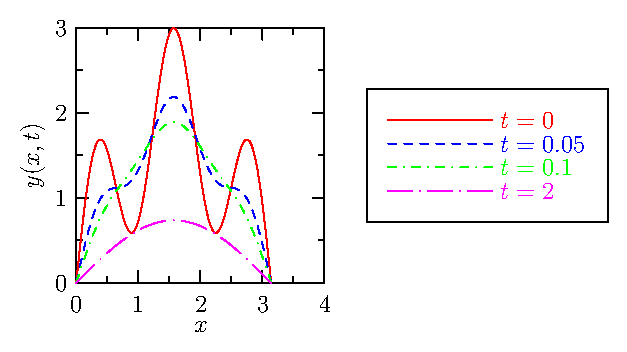
\includegraphics{201/heat1}
      \caption{The temperature at different times with initial conditions
        given in \eqref{heat1ic}. Notice that the $\sin(5x)$ term, which
        decays like $e^{-25 \b t}$, is relevant only for small $t$. }
      \label{heat1}
    \end{center}
  \end{figure}
}


\section{Non-homogeneous constant boundary conditions}

Suppose that the boundary conditions were instead
\begin{align*}
y(0,t)=A, \qquad y(\pi,t)=B.
\end{align*}
Notice that these conditions match the case $K_n=0$ with
\begin{align*}
y(x,t)=\frac{B-A}{\pi}x+A.
\end{align*}
This obeys the heat equation, since
\begin{align*}
\frac{\partial^2}{\partial x^2}(mx+b)=0= \pp{}{t}(mx+b),
\end{align*}
and is independent of $t$, i.e.\ it is a steady state solution. Then, setting
\begin{align*}
g(x) = f(x) - \(A+ \frac{B-A}{\pi}x\),
\end{align*}
\begin{align}
\label{diribc}
y(x,t)=A + \frac{B-A}{\pi}x +
\frac{2}{\pi}
\sum_{n=1}^\infty\(\int_{0}^\pi g(x)\sin(nx)dx\) e^{-\b n^2t} \sin(nx)
\end{align}
matches both the initial and boundary conditions.

\oexample{
  Solve the initial boundary problem
  \begin{align*}
  \label{heat3ic}
  \pp{y}{t} = \b \pptwo{y}{x}, \qquad y(0)=1, \quad y(\pi)=1+\pi,
  \quad y(x,0)=f(x)=x^2 +x +1
  \end{align*}
  for $y(x,t)$.

}{
  The steady-state solution is $x+1$. Let
  \begin{align*}
  g(x) = f(x) -(x+1) = x^2
  \end{align*}
  Then,
  \begin{align*}
  y(x,t) = 1 + x + \sum_{n=1}^\infty T_n(0) e^{-\b n^2 t} \sin(nx).
  \end{align*}
  And in order to satisfy $y(x,0)=1+x+x^2$, we have
  \begin{align*}
  x^2 = \sum_{n=1}^\infty T_n(0) \sin(nx).
  \end{align*}
  The coefficients are given by the formula
  \begin{align*}
  T_n(0) &=& \frac{2}{\pi} \int_0^\pi x^2 \sin(nx) \, dx
  \\\nonumber
  &=& \frac{2}{\pi}\[\left.x^2 \frac{-\cos(nx)}{n} \right|_0^\pi
  + \frac{2}{n}\int_0^\pi x \cos(nx)dx\]
  \\\nonumber
  &=& \frac{2}{n\pi}\[ -\pi^2\cos(n\pi)+2(\left.\frac{x \sin(nx)}{n}
  \right|_0^\pi
  - \frac{1}{n}\int_0^\pi\sin(nx)dx)  \]
  \\\nonumber
  &=& \frac{-2\pi}{n}\cos(n\pi)-\frac{4}{n^3\pi} \left.-\cos(nx) \right|_0^\pi
  = \frac{-2\pi}{n}(-1)^n + \frac{4(\(-1)^n-1\)}{n^3\pi}
  \end{align*}
  The solution is therefore
  \begin{align*}
  y(x,t) = 1+x+
  \sum_{n=1}^\infty \[\frac{-2\pi}{n}(-1)^n + \frac{4(\(-1)^n-1\)}{n^3\pi}\]
  e^{-\b n^2 t}\sin(nx).
  \end{align*}
% Useless figure
%  as can be seen in figure \ref{heat3}. \qed
%  \begin{figure}[htbp]
%    \begin{center}
%      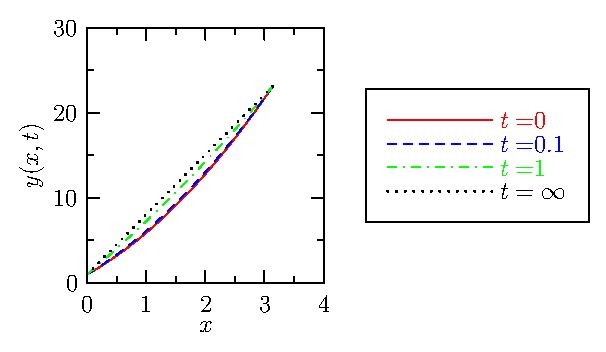
\includegraphics{201/heat3}
%      \caption{The temperature at different times for the system given in
%        \eqref{heat3ic}.}
%      \label{heat3}
%    \end{center}
%  \end{figure}

}
% This lab is too long!
%\section{A more complicated example}
%
%\oexample{
%  The heat in a rod obey the equation
%  \be
%  \pp{y}{t}=\pptwo{y}{x}.
%  \end{align}
%  Given the boundary conditions
%  \begin{align}
%  \label{heat2ic}
%  y(0,t)=1 \qquad y(\pi,t)=e^\pi
%  \end{align}
%  and the and the initial condition $y(x,0)=e^x$, find $y(x,t)$.\\
%}{
%  The solution is given by
%  \begin{align}
%  y(x,t)&=&1 + \frac{e^\pi-1}{\pi}x +
%  \sum_{n=1}^\infty T_n(0) e^{-n^2t} \sin(nx),
%  \\
%  T_n(0)&=&\frac{2}{\pi}\int_{0}^\pi g(x)\sin(nx)dx,
%  \\
%  g(x)&=&e^x - 1 - \frac{e^\pi-1}{\pi}x.
%  \end{align}
%  From equation \eqref{Fourierx}, we have
%  \begin{align}
%  x = 2 \sum_{n=1}^\infty  \frac{(-1)^{n+1}}{n} \sin(nx)
%  \end{align}
%  To find the Fourier sine-series for $e^x$, we must compute
%  \begin{align}
%  a_n = \frac{2}{\pi}\int_0^\pi e^x \sin(nx) \, dx
%  = \frac{2}{\pi}\left.\frac{e^x\(\sin(nu) - n \cos(nu)\)}{n^2+1}\right|_0^\pi
%  = \frac{2}{\pi}\frac{n(1 - (-1)^ne^\pi)}{n^2+1}
%  \end{align}
%  Also, the Fourier series for $1$ over $x\in(-\pi,\pi)$ has coefficients
%  \begin{align}
%  \frac{2}{\pi}\int_0^\pi \sin(nx) = \frac{2}{n\pi}\left.\cos(nx) \right|_0^\pi
%  = \frac{2\((-1^n)-1\)}{n\pi},
%  \end{align}
%  so, over $x\in(0,\pi)$,
%  \begin{align}
%  1 = \sum_{n=1}^\infty \frac{2\((-1^n)-1\)}{n\pi} \sin(nx).
%  \end{align}
%
%  Noting that the Fourier series is a linear, so we can add the series
%  together:
%  \begin{align}
%  e^x - 1- \frac{e^\pi}{\pi}x
%  &=& \sum_{n=1}^\infty \frac{2}{\pi}n\frac{1 - (-1)^ne^\pi}{n^2+1} \sin(nx)
%  - \frac{e^\pi-1}{\pi} 2 \sum_{n=1}^\infty  \frac{(-1)^{n+1}}{n} \sin(nx)
%  \\ \nonumber
%  &&-\sum_{n=1}^\infty \frac{2\((-1^n)-1\)}{n\pi} \sin(nx)
%  \\ \nonumber
%  &=&\sum_{n=1}^\infty \(\frac{2}{\pi}\frac{n(1 - (-1)^ne^\pi)}{n^2+1}
%  -\frac{e^\pi-1}{\pi}2 \frac{(-1)^{n+1}}{n}- \frac{2\((-1^n)-1\)}{n\pi}\)
%  \sin(nx).
%  \end{align}
%  Now, this is all a bit messy, but we do end up with the solution
%  \begin{align}
%  y(x,t) = 1 &+& \frac{e^\pi-1}{\pi}x
%  \\ \nonumber
%  &+&
%  \sum_{n=1}^\infty \(\frac{2}{\pi}\frac{n(1 - (-1)^ne^\pi)}{n^2+1}
%  -2 \frac{e^\pi-1}{\pi} \frac{(-1)^{n+1}}{n}- \frac{2\((-1^n)-1\)}{n\pi}\)
%    e^{-n^2t} \sin(nx),
%  \end{align}
%  as can be seen in figure \ref{heat2}. \qed
%  \begin{figure}[htbp]
%    \begin{center}
%      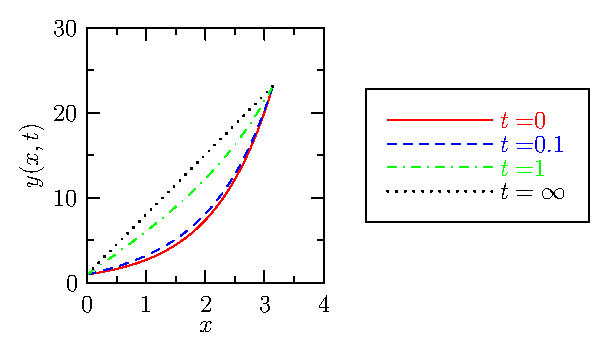
\includegraphics{201/heat2}
%      \caption{The temperature at different times with initial conditions
%        given in \eqref{heat2ic}.}
%      \label{heat2}
%    \end{center}
%  \end{figure}
%}



\section{Problems}

\begin{enumerate}
  \item
    Show that equation \eqref{diribc} does indeed solve the heat equation
    with the given boundary and initial conditions.
  \item
    An inanimate carbon rod of length $\pi$ is hit with a ``laser'',
    transferring an amount of heat $H$ to a point at its centre. That is, the
    initial temperature distribution along its length is given by
    \begin{align*}
    y(x,0)=H\delta\(x-\frac{\pi}{2}\).
    \end{align*}
    If the ends of the rod are kept at constant temperature $0$, and the
    temperature in the rod obeys the relationship
    \begin{align*}
    \pp{y}{t} = \beta \frac{\partial^2 y}{\partial x^2},
    \end{align*}
    find $y(x,t)$ for all $t\geq 0$.
    \hidesolution{
      Following the above procedure,
      \begin{align*}
      y(x,t)=\frac{2}{\pi}
      \sum_{n=1}^\infty T_n(0) e^{-kn^2t} \sin(nx)
      \end{align*}
      with
      \begin{align*}
      T_n(0) &=& \frac{2}{\pi}\int_0^\pi H \d\(x-\frac{\pi}{2} \) \sin(nx) \, dx
      \\
      &=& \frac{2H}{\pi} \sin\(\frac{n\pi}{2}\)
      \\
      &=& \frac{2H}{\pi}
      \left\{ \begin{array}{ll}
        0,           & \mbox{if $n=2m$}\\
        \sin\(m\pi+ \frac{\pi}{2}\), & \mbox{if $n=2m+1$}
      \end{array} \right.
      \\
      &=& \frac{2H}{\pi}
      \left\{ \begin{array}{ll}
        0,           & \mbox{if $n=2m$}\\
        (-1)^m, & \mbox{if $n=2m+1$}.
      \end{array} \right.
      \end{align*}
      The solution is then given by
      \begin{align*}
      y(x,t) = \frac{2H}{\pi} \sum_{m=0}^\infty (-1)^m e^{-4\beta m^2 t} \sin(2mx)
      \end{align*}
    }
  \item
    \emph{Neumann boundary conditions} specify the value of the function at
    the boundary, e.g. $y(0,t)=A$, $y(\pi,t)=B$ with $A$ and $B$ constant.
    We showed that the set of Eigenfunctions given by equation
    \eqref{Eigenfunction} must be $\{\sin(nx),n=1,2,\dots\}$ in this case.
    If the boundary conditions were instead \emph{Dirichlet boundary conditions}
    such as
    \begin{align*}
    \left.\pp{y(x,t)}{x}\right|_{x=0}=0, \qquad
        \left.\pp{y(x,t)}{x}\right|_{x=\pi}=0,
    \end{align*}
    what are the Eigenfunctions?


\end{enumerate}


\chapter{Tables}

\section{Table of Integrals}

\begin{align}\nonumber
&\int u dv = uv - \int v du
&
\\\nonumber
& \int \cos x dx = -\sin x
& \int \sin x dx = \cos x
\\\nonumber
& \int \tan x dx  = -\ln\abs{\cos x}
&
\\\nonumber
& \int \sin^2 x dx = \frac{1}{2}x - \frac{1}{4}\sin 2x
& \int \cos^2 x dx = \frac{1}{2}x + \frac{1}{4}\sin 2x
\\\nonumber
& \int \tan^2 x dx  = \tan x - x
&
\\\nonumber
& \int \sin^n x dx = -\frac{\sin^{n-1}x\cos{x}}{n}
+ \frac{n-1}{n}\int\sin^{n-2}xdx
&
\\\nonumber
& \int \cos^n x dx = \frac{\cos^{n-1}x\sin x}{n}
+ \frac{n-1}{n}\int \cos^{n-2}x dx
&
\\\nonumber
& \int \sin ax \sin bx dx = - \frac{\sin(a+b)x}{2(a+b)}
  + \frac{\sin(a-b)x}{2(a-b)},\quad a^2\neq b^2
&
\\\nonumber
& \int \cos ax \cos bx dx = \frac{\sin(a+b)x}{2(a+b)}
+ \frac{\sin(a-b)x}{2(a-b)},\quad a^2\neq b^2
&
\\\nonumber
& \int \sin ax \cos bx dx = -\frac{\cos(a+b)x}{2(a+b)}
- \frac{\cos(a-b)x}{2(a-b)},\quad a^2\neq b^2
&
\\\nonumber
& \int \sec^2 x dx = \tan x
& \int \csc^2 x dx = -\cot x
\\\nonumber
& \int \sec x \tan x  dx = \sec x
&
\\\nonumber
& \int \frac{dx}{\sqrt{a^2-x^2}}= \arcsin\frac{x}{a}
& \int \frac{dx}{x\sqrt{x^2-a^2}}= \frac{1}{a}\arccos\frac{a}{x}
\\\nonumber
&\int \frac{dx}{a^2+x^2} = \frac{1}{a}\arctan\frac{x}{a},
&
\\\nonumber
& \int \frac{dx}{a^2-x^2} = \frac{1}{2a}\ln\abs{\frac{x+a}{x-a}},
& \int \frac{dx}{\sqrt{a^2+x^2}} = \ln\abs{x+\sqrt{x^2+a^2}}
\\\nonumber
& \int \sinh x dx = \cosh x
& \int \cosh x dx = \sinh x
\\\nonumber
& \int e^{ax}\sin nx dx = \frac{e^{ax}\(a \sin nx - n \cos nx \) }{a^2+n^2 }&
\\\nonumber
& \int e^{ax}\cos nx dx = \frac{e^{ax}\(a \cos nx + n \sin nx \) }{a^2+n^2 }
&
\end{align}

\section{Table of Laplace Transforms}

\label{tableolap}
\begin{center}
\begin{tabular}{ l |  l }
  $f(t)$ & $\mathcal{L}(f) = F(s)$  \\
  \hline
  $f'(t)$ & $sF(s) -f(0)$\\
  $f''(t)$ & $s^2F(s) -sf(0) - f'(0)$\\
  $f^{(n)}(t)$ & $s^nF(s) -s^{n-1}f(0)-\dots - f^{(n-1)}(0)$\\
  $t$ & $\frac{1}{s}$ \\
  $t^n$ & $\frac{n!}{s^{n+1}}$ \\
  $e^{\a t}$ & $\frac{1}{s-\a} $ \\
  $e^{\a t}f(t) $ & $F(s-\a) $ \\
  $f(ct) $ & $\frac{1}{c}F\(\frac{s}{c}\) $ \\
  $\sin(\beta t)$ & $\frac{\beta}{s^2 + \beta^2} $ \\
  $\cos(\beta t)$ & $\frac{s}{s^2 + \beta^2} $ \\
  $\sinh(\beta t)$ & $\frac{\beta}{s^2 - \beta^2} $ \\
  $\cosh(\beta t)$ & $\frac{s}{s^2 - \beta^2} $ \\
  $e^{\alpha t}\sin(\beta t)$ & $\frac{\beta}{(s-\alpha)^2 + \beta^2} $ \\
  $e^{\alpha t}\cos(\beta t)$ & $\frac{s-\alpha}{(s-\alpha)^2 + \beta^2} $ \\
  $u_c(t)$ & $\frac{e^{-cs}}{s}$ \\
  $u_c(t)f(t-c)$ & $e^{-cs}F(s)$ \\
  $\delta(t)$ & $1$ \\
  $\int_0^t f(t-\tau) g(\tau) \,d\tau \doteq f*g$ & $F(s)G(s) $ \\
  $f(t)$ with $f(t+T)=f(t)$ & $\frac{\int_0^Tf(t) e^{-st}dt}{1-e^{-sT}}$\\
  $t^n f(t)$ & $(-1)^n \frac{d^n}{ds^n} F(s)$\\
\end{tabular}\\
\end{center}


\section{Table of Taylor Series}
\begin{align}\nonumber
& f(x) = f(a) + f'(a)(x-a) + \frac{f''(a)}{2!} + \dots
+ \frac{f^{(n)}(a)}{n!}(x-a)^n + \dots
%&
%&
\\\nonumber
& e^x = \sum_{n=0}^\infty \frac{x^n}{n!}
\qquad \sin x = \sum_{n=0}^\infty \frac{(-1)^n x^{2n+1}}{(2n+1)!}
\qquad \sin x = \sum_{n=0}^\infty \frac{(-1)^n x^{2n+1}}{(2n+1)!}
\\\nonumber
&\tan x = x + \frac{1}{3}x^3 + \frac{2}{15}x^5 + \frac{17}{315}x^7
+ \frac{62}{2835}x^9 + \dots
\\\nonumber
&\arcsin x = x + \frac{1}{2}\frac{x^3}{3}
+ \frac{1\cdot 3}{2\cdot 4}\frac{x^5}{5}
+ \frac{1\cdot3\cdot5}{2\cdot4\cdot6}\frac{x^7}{7} + \dots
\\\nonumber
&\arctan x = \sum_{n=0}^\infty (-1)^n \frac{x^{2n+1}}{2n+1}
\\\nonumber
&\frac{1}{1-x} = \sum_{n=0}^\infty x^n
\qquad \ln(1-x) = -\sum_{n=1}^\infty \frac{x^n}{n}
\end{align}

\end{document}
